%%%%%%%%%%%%%%%%%%%%%%%%%%%%%%%%%%%%%%%%%
% American Geophysical Union (AGU)
% LaTeX Template
% Version 1.0 (3/6/13)
%
% This template has been downloaded from:
% http://www.LaTeXTemplates.com
%
% Original author:
% The AGUTeX class and agu-ps referencing style were created and are owned 
% by AGU: http://publications.agu.org/author-resource-center/author-guide/latex-formatting-toolkit/
%
% This template has been modified from the blank AGU template to include
% examples of how to insert content and drastically change commenting. The
% structural integrity is maintained as in the original blank template.
%
% Important notes: 
% This template retains extensive commenting from the AGU template. It is heavily 
% advised you read these comments and follow them in order to insure a speedy 
% submission process.
%
%%%%%%%%%%%%%%%%%%%%%%%%%%%%%%%%%%%%%%%%%

%%%%%%%%%%%%%%%%%%%%%%%%%%%%%%%%%%%%%%%%%%%%%%%%%%%%%%%%%%%%%%%%%%%%%%%%%%%%
% AGUtmpl.tex: this template file is for articles formatted with LaTeX2e,
% Modified March 2013
%
% This template includes commands and instructions
% given in the order necessary to produce a final output that will
% satisfy AGU requirements.
%
% PLEASE DO NOT USE YOUR OWN MACROS
% DO NOT USE \newcommand, \renewcommand, or \def.
%
% FOR FIGURES, DO NOT USE \psfrag or \subfigure.
%
%%%%%%%%%%%%%%%%%%%%%%%%%%%%%%%%%%%%%%%%%%%%%%%%%%%%%%%%%%%%%%%%%%%%%%%%%%%%
%
% All questions should be e-mailed to latex@agu.org.
%
%%%%%%%%%%%%%%%%%%%%%%%%%%%%%%%%%%%%%%%%%%%%%%%%%%%%%%%%%%%%%%%%%%%%%%%%%%%%

% Step 1: Set the \documentclass

% There are two options for article format: two column (default) and draft.

% PLEASE USE THE DRAFT OPTION TO SUBMIT YOUR PAPERS.
% The draft option produces double spaced output.

% Choose the journal abbreviation for the journal you are submitting to:

% jgrga	JOURNAL OF GEOPHYSICAL RESEARCH
% gbc	GLOBAL BIOCHEMICAL CYCLES
% grl		GEOPHYSICAL RESEARCH LETTERS
% pal	PALEOCEANOGRAPHY
% ras	RADIO SCIENCE
% rog	REVIEWS OF GEOPHYSICS
% tec	TECTONICS
% wrr	WATER RESOURCES RESEARCH
% gc		GEOCHEMISTRY, GEOPHYSICS, GEOSYSTEMS
% sw	SPACE WEATHER
% ms	JAMES
%
%
%
% (If you are submitting to a journal other than jgrga,
% substitute the initials of the journal for "jgrga" below.)

\documentclass[draft,jgr]{AGUTeX}

% To create numbered lines:

% If you don't already have lineno.sty, you can download it from http://www.ctan.org/tex-archive/macros/latex/contrib/ednotes/ (or search the internet for lineno.sty ctan), available at TeX Archive Network (CTAN). Take care that you always use the latest version.

% To activate the commands, uncomment \usepackage{lineno} and \linenumbers*[1]command, below:

\usepackage{lineno,url}
\linenumbers*[1]
%\usepackage{hyperref}


%  To add line numbers to lines with equations:
%  \begin{linenomath*}
%  \begin{equation}
%  \end{equation}
%  \end{linenomath*}

%%%%%%%%%%%%%%%%%%%%%%%%%%%%%%%%%%%%%%%%%%%%%%%%%%%%%%%%%%%%%%%%%%%%%%%%%
% Figures and Tables

% DO NOT USE \psfrag or \subfigure commands.

%  Figures and tables should be placed AT THE END OF THE ARTICLE, after the references.

%  Uncomment the following command to include .eps files (comment out this line for draft format):
%\usepackage[dvips]{graphicx}
\usepackage{graphicx}

% Substitute one of the following for [dvips] above if you are using a different driver program and want to proof your illustrations on your machine:
% [xdvi], [dvipdf], [dvipsone], [dviwindo], [emtex], [dviwin],
% [pctexps],  [pctexwin],  [pctexhp],  [pctex32], [truetex], [tcidvi],
% [oztex], [textures]

%  Uncomment the following command to allow illustrations to print when using Draft:
\setkeys{Gin}{draft=false}

% See how to enter figures and tables at the end of the article, after references.

%----------------------------------------------------------------------------------------
%	RUNNING HEAD AND CORRESPONDING AUTHOR
%----------------------------------------------------------------------------------------

% Author names in capital letters:
\authorrunninghead{COOK ET AL.}

%------------------------------------------------

% Shorter version of title entered in capital letters:
\titlerunninghead{MEDITERRANEAN DROUGHT}

%------------------------------------------------

% Corresponding author mailing address and e-mail address:
\authoraddr{Corresponding author: Benjamin I Cook, NASA Goddard Institute for Space Studies, New York, New York, USA. (benjamin.i.cook@nasa.gov)}

%----------------------------------------------------------------------------------------

\begin{document}

%----------------------------------------------------------------------------------------
%	TITLE
%----------------------------------------------------------------------------------------

\title{Mediterranean drought variability over the last millennium}

%----------------------------------------------------------------------------------------
%	AUTHORS AND AFFILIATIONS
%----------------------------------------------------------------------------------------

% Use \author{\altaffilmark{}} and \altaffiltext{}

% \altaffilmark will produce footnote; matching \altaffiltext will appear at bottom of page.

\authors{Benjamin I Cook\altaffilmark{1,2},
Kevin J Anchukaitis\altaffilmark{3,4,5,6}, 
Ramzi Touchan\altaffilmark{4}, 
David M Meko\altaffilmark{4}, and
Edward R Cook \altaffilmark{6}}

\altaffiltext{1}{NASA Goddard Institute for Space Studies, New York, New York, USA.}

\altaffiltext{2}{Ocean and Climate Physics, Lamont-Doherty Earth Observatory, Palisades, New York, USA.}

\altaffiltext{3}{School of Geography and Development, University of Arizona, Tucson, Arizona, USA.}

\altaffiltext{4}{Laboratory of Tree-Ring Research, University of Arizona, Tucson, Arizona, USA.}

\altaffiltext{5}{Woods Hole Oceanographic Institution, Woods Hole, Massachusetts, USA.}

\altaffiltext{6}{Tree Ring Laboratory, Lamont-Doherty Earth Observatory, Palisades, New York, USA.}

%----------------------------------------------------------------------------------------
%	ABSTRACT
%----------------------------------------------------------------------------------------
\pagebreak
% Do NOT include any \begin...\end commands within the body of the abstract.
% 250 word limit in abstract for JGR
\begin{abstract}
Recent droughts in the Mediterranean have highlighted concerns that anthropogenic climate change may be contributing to observed drying trends, but the full range of natural climate variability in the region is still poorly understood. Here, we analyze 900 years (1100--2012) of Mediterranean drought variability in the Old World Drought Atlas (OWDA), a spatiotemporal tree-ring based reconstruction of the June-July-August self calibrating Palmer Drought Severity Index. In the Mediterranean, the OWDA is highly correlated with spring precipitation (April--June), the North Atlantic Oscillation (January--April), the Scandinavian Pattern (January--March), and the East Atlantic Pattern (April--June). Drought variability in the basin shows significant east-west coherence on multi-decadal to centennial time scales, contrary to previous analyses. We also find significant North-South antiphasing in the eastern Mediterranean, with a tendency for the Black Sea region (e.g., Greece, Anatolia, the Balkans, etc) to be wet when coastal Libya, the southern Levant, and the Middle East are dry, possibly related to variability in the North Atlantic Oscillation. Recent droughts are centered in the western Mediterranean, Greece, and the Levant region. Events of similar magnitude in the western Mediterranean and Greece are apparent in the OWDA back to 1100 CE, but the most recent 15-year drought in the Levant (1998--2012) appears as the driest such period in the record. Estimating sampling uncertainties using a Monte-Carlo approach, we conclude there is an 89\% likelihood that the recent Levant drought is drier than any comparable period of the last 900 years, possibly indicating the emergence of an anthropogenically forced drying signal. 
\end{abstract}

%----------------------------------------------------------------------------------------
%	ARTICLE CONTENT
%----------------------------------------------------------------------------------------

% The body of the article must start with a \begin{article} command
% \end{article} must follow the references section, before the figures and tables.

\begin{article}

\section{Introduction}
\noindent Climate change impacts on water resources are a significant concern in the regions surrounding the Mediterranean Sea \citep{Iglesias2007,GarciaRuiz2011}, an area including southern Europe, Northern Africa, and the Levant (Cyprus, Israel, Jordan, Lebanon, Palestine, Syria, Turkey) region of the Middle East. Projections from climate models almost uniformly point towards drying in the Mediterranean from increased greenhouse gas forcing in the coming decades \citep{Giorgi2008,IPCC_Collins:etal2013,Seager2014med}, part of an overall trend towards desiccation and poleward expansion of subtropical dry zones \citep{Held:2006,Seager2010b}. Indeed, analyses of recent climate trends in the region suggest that this process may have already begun \citep{GarciaRuiz2011,Gleick2014,Hoerling2012c,Kelley2012,Kelley2015}. 

\indent However, a more complete understanding of natural Mediterranean drought variability and anthropogenically forced moisture trends requires comparisons with long-term variability that is not available from relatively short instrumental records. To this end, the paleoclimate community has been active throughout this region, developing estimates of Common Era drought variability from a variety of proxies, including tree-rings \citep{Chbouki:etal1995,Glueck:Stockton2001,Touchan:etal2003,Akkemik:Aras2005,Touchan:etal2005,Esper:etal2007a,Andreu:etal2007,Nicault:etal2008,Touchan:etal2008a,Buntgen:etal2010,Touchan:etal2010a,Kose:etal2011,Touchan:etal2014a}, sediment cores \citep[e.g.,][]{Jones:etal2006,Roberts:etal2012,Moreno:etal2012}, and speleothems \citep[e.g.,][]{Jex:etal2011,Wassenburg:etal2013}. To date, however, there is little consensus across these different records regarding the character and dominant drivers of drought variability across the basin over the last millennium. In particular, there are extant uncertainties regarding how widespread droughts are in the Mediterranean \citep{Roberts:etal2012}, the magnitude and timing of long-term trends and centennial-scale variability \citep{Esper:etal2007a,Touchan:etal2010a,Wassenburg:etal2013}, and how seasonal signals and large-scale climate modes are reflected in proxy reconstructions \citep{Touchan:etal2014a,Touchan:etal2014b,Seim:etal2014}.

\indent Given these uncertainties, the development and analyses of new large-scale reconstructions is imperative for improving our understanding of regional climate dynamics in the Mediterranean region. Here, we use a spatially resolved tree-ring based field reconstruction of European and Mediterranean drought to investigate the dominant spatial and temporal patterns of drought variability across the basin over the last millennium. Specifically, our analysis addresses three primary research questions: 1) What are the dominant modes of hydroclimate variability in the Mediterranean? 2) How spatially coherent are drought events across the Mediterranean basin? and 3) How do recent droughts compare to long-term hydroclimate variability over the last millennium?
%------------------------------------------------

\section{Materials and Methods}
\subsection{The Old World Drought Atlas}
\noindent The Old World Drought Atlas \citep[OWDA;][]{CookOWDA2015} is a new, tree-ring based reconstruction of summer season (June-July-August, JJA) self calibrating Palmer Drought Severity Index (scPDSI) \citep{Schrier2013}. The OWDA uses 106 tree-ring chronologies to reconstruct scPDSI at 5,414 half degree grid points for the entire Common Era over the European-Mediterranean domain (27\textsuperscript{o}N--71\textsuperscript{o}N, 12\textsuperscript{o}W--45\textsuperscript{o}E). The reconstruction uses the point-by-point method \citep{Cook1999,CookER2013} with a search radius of 1000 kilometers around each target grid point. Grid cell scPDSI is reconstructed from the proxy predictor series within the search radius, but the tree-ring proxies are effectively weighted by the principal components regression such that those that covary most strongly with observations have the greatest influence on the reconstructions. Proxy site locations in the Mediterranean portion of the OWDA (30\textsuperscript{o}N--47\textsuperscript{o}N, 10\textsuperscript{o}W--45\textsuperscript{o}E) are shown in Figure 1, along with the approximate start date of the various records. We restrict our analysis to 1100--2012 CE, the interval during which the Mediterranean domain is reasonably well sampled by proxy sites. Values in the OWDA through 1978 are reconstructed from tree-ring chronologies, while from 1979--2012 the OWDA incorporates the instrumental scPDSI. 

\indent  The scPDSI is a modification of the original PDSI formulation of \cite{Palmer1965}, a locally normalized drought index incorporating changes in supply (precipitation), demand (evapotranspiration), and storage (soil moisture). PDSI has an inherent memory timescale of 12--18 months \citep{Guttman1998,Vicente2010}, allowing the JJA target of the OWDA to incorporate climate information from the previous winter and spring, the main seasons of moisture supply to the Mediterranean. The scPDSI used as the target for the OWDA reconstruction \citep{Schrier2013} is calculated from version TS3.21 of the high-resolution CRU climate grids \citep{Harris2014}, incorporates a snow module, and uses the Penman-Monteith formulation for calculating potential evapotranspiration \citep{Xu2002}. .

\subsection{Climate Data}
\noindent Monthly precipitation data used in the analyses are from the high-resolution CRU gridded climate data \citep[TS3.21,][]{Harris2014}. We also use monthly average indices from the Climate Prediction Center from climate modes previously shown to have an influence on Mediterranean climate \citep{Sousa2011}. The North Atlantic Oscillation \citep[NAO;][]{Hurrell1995} consists of a north-south dipole in atmospheric pressure between Greenland and the subtropical North Atlantic, with positive phases typically associated with below-average precipitation in the Mediterranean and southern Europe. The Scandinavian Pattern \citep[SCA;][]{Bueh2007} is centered over Scandinavia, with positive height anomalies in this region causing above-average precipitation across central and southern Europe. The East Atlantic Pattern \citep[EA;][]{Barnston1987} is similar to the NAO, consisting of a north-south anomaly dipole in the Atlantic. Unlike the NAO, however, the EA has stronger connections to the subtropical ridge. Positive phases of the EA are linked to below average precipitation across southern Europe. For the CRU precipitation data and the climate indices, we restrict our analysis for the most recent period when data quality and availability is highest (1950--2012).

\subsection{Analyses}
\noindent We use Spearman's rank correlations to assess the statistical relationship between reconstructions, observations, and indices.  Spearman's is a non-parametric alternative to the Pearson product-moment correlation that is less sensitive to outliers. We also conduct spectral and spectral coherency analyses using a multi-taper approach \citep{Thomson:1982,Chave:etal1987,Mann:Lees1996,Czaja:Marshall2001,Huybers:2004} with significance levels estimated using a non-parametric Monte Carlo procedure with red noise (AR1) conditioned on the original data. We also use wavelet coherency analyses \citep{Marauan2004,Maraun2007} to investigate time-varying coherency and phase between various drought series. In some figures, the time series were smoothed using a 10-year loess fit \citep{Cleveland:etal1988} to emphasize low frequency variability, although all statistical analyses were conducted on the original (unfiltered) data.

\section{Results}
\subsection{Climate Signals in the OWDA}
\noindent Correlations between winter (January--March; JFM) and spring (April--June) precipitation and the tree-ring reconstructed JJA scPDSI are uniformly positive across the basin (Figure 2). The strongest correlations with JFM precipitation are localized in Spain and Morocco in the western Mediterranean and the Levant region in the eastern basin.  AMJ precipitation correlations are more uniform and strongly positive across nearly the entire Mediterranean, suggesting that the summer season soil moisture variability, reflected in the OWDA and the underlying tree growth, is driven primarily by spring precipitation \citep[c.f.][]{Touchan:etal2014a}.

\indent Climate mode correlations with the CRU precipitation data or the OWDA scPDSI (Figure 3) are consistent in sign, but generally stronger in the precipitation data. The weaker OWDA scPDSI correlations are expected for at last two reasons. First, these climate modes reflect shifts in atmospheric circulation that have a direct impact on precipitation by modulating, for example, storm track positions and moisture convergence. Circulation impacts on the scPDSI will be by definition more indirect, as the scPDSI is computed based on the anomalies of a variety of variables that influence soil moisture. Additionally, up to year 1978, the scPDSI is reconstructed as a scaled linear function of the underlying tree-ring proxies, which imparts additional uncertainties on the estimates of scPDSI. 

\indent The influence of the NAO is strongest in winter and early spring (January--April; JFMA). Positive phases of the NAO cause drying across the northern reaches of the Mediterranean basin, from Spain and Morocco across to the Balkans and western Turkey, while favoring wetter conditions in coastal regions of Libya, Egypt, and the Levant.  Consistent with both the instrumental observations \citep[e.g.][]{Lamb:etal1997,Knippertz:etal2003} and the underlying controls on tree growth \citep{Touchan:etal2008a,Touchan:etal2008b,Panayotov:etal2010}, the influence of the NAO in the OWDA is strongest in the far western part of the domain and the Balkans. The largest influence of the SCA pattern is during the winter (JFM), with positive phases increasing moisture across most of the basin. The SCA correlation with the OWDA is substantially weaker, consistent with previously analyses (Figure 2) demonstrating the much stronger connection between the OWDA and spring season, rather than winter, precipitation. Unlike the previous two modes, the influence of the EA is highest during the spring (AMJ), causing widespread drying across the basin with, notably, similar magnitude correlations with both precipitation and scPDSI.

\subsection{Drought Variability in the OWDA}
\noindent Figure 4 shows OWDA scPDSI averaged over the Mediterranean domain and the fractional land area in drought (scPDSI$\le-1$) for each year from 1100--2012. Inter-annual variability (standard deviation) in the scPDSI is 0.54 standardized PDSI units and, on average, 29\% of the basin experiences drought conditions in any given year. Highlighted are several example periods of persistent multi-year droughts and pluvials (Figure 4, grey bars). Noticeably absent are any extended multi-decadal (30-year or longer) `megadroughts', a characteristic feature of North American drought variability during the Medieval Climate Anomaly (approximately before 1300 CE) \citep[e.g.,][]{CookER2010b} and previously inferred from Moroccan tree-rings \citep{Esper:etal2007a}.

\indent The spatial expression of the six highlighted periods of widespread drought (and one pluvial) are shown in Figure 5. The most dramatic wet interval was a nearly two-decade long period from 1125--1142 CE, with sustained wet conditions in modern day Spain, Morocco, Algeria, Tunisia, Italy, the Balkans, and Turkey. This pluvial coincided with an extended period (1118-1179 CE) of low flows in the Upper Colorado River Basin (UCRB) in North America \citep[the most persistent dry period in that region over the last millennium;][]{Meko:etal2007a}, severe drought in the Sacramento River Basin \citep{Meko2012}, and widespread drought across most of North America \citep{Cook2014}. This synchrony may suggest some large-scale persistent anomaly in atmospheric circulation across the Atlantic, possibly related to shifts in Atlantic sea surface temperatures \citep{Hu2012}. Among the five highlighted persistent drought events, there is a tendency for simultaneous drought in the extreme western (Spain, Morocco, Algeria, Tunisia) and eastern (Balkans, Greece, Turkey) ends of the basin. This is somewhat contrary to previous analyses of other proxy records in the region, which have suggested instead a tendency for an antiphased dipole in hydroclimate variability between these two regions \citep[e.g.,][]{Roberts:etal2012}. The basin-wide synchrony found in these example events is further confirmed by compositing all years when at least 40\% or 50\% of the basin is in drought (Figure 6). Here again, we observe the major poles of synchronous and severe drought during these years of widespread drought are centered over the opposite ends of the basin. There is, however, evidence for antiphasing in the eastern end of the basin, where there is a tendency for Libya, Egypt and the southern Levant to be wet or near normal when Greece and Anatolia are in drought. This meridional dipole structure bears some resemblance to the NAO correlation patterns with precipitation and scPDSI (Figure 3).

\subsection{Spatial Synchrony}
\noindent To further investigate the tendency for synchronous hydroclimate variability across the basin, we averaged scPDSI from the OWDA over three regions: the western Mediterranean (WestMED; 32\textsuperscript{o}N--42\textsuperscript{o}N, 10\textsuperscript{o}W--0\textsuperscript{o}E), the eastern Mediterranean (EastMED; 36\textsuperscript{o}N--41\textsuperscript{o}N, 20\textsuperscript{o}E--37\textsuperscript{o}E), and an area encompassing coastal Egypt, the southern Levant, and other areas of the Middle East (MidEast; 30\textsuperscript{o}N--34\textsuperscript{o}N, 33\textsuperscript{o}E--47\textsuperscript{o}E). The first two areas (WestMED and EastMED) correspond to approximately the same areas used in the analysis of \citet{Roberts:etal2012}. Point-by-point correlations (Figure 7) between these three indices and the OWDA are strongly positive at the local level, as expected, decaying in magnitude outside of the averaging regions. For WestMED the correlations remain mostly positive, or near zero, across the entire basin. EastMED, however, shows strong negative correlations over Libya, Egypt, and the Levant while MidEast is negatively correlated with a large region surrounding the Black Sea. As with the drought composites (previous section), these results again suggest a strong tendency for meridional antiphasing in hydroclimate in the eastern Mediterranean Basin, with a pattern similar to what would be expected due to precipitation responses to variations in the NAO.\\
\indent Spectral analyses of WestMED and EastMED show significant power in both series at high (inter-annual) and low (decadal to multidecadal) frequencies (Figure 8). Both have significant peaks at about 3--4 years, with EastMED additionally peaking at decadal frequencies and WestMED covering a broader range of multi-decadal bands. The two regions also overlap in their power at around 70 years, though EastMED is only marginally significant at the 90\textsuperscript{th} percentile. A coherency spectra analysis between the two regional indices demonstrates highly significant coherence between the two regions over inter-annual and decadal timescales (Figure 9). Notably, there is also a broad band of coherence between the two regions at multi-decadal and centennial timescales (30 to 130 years), despite no significant spectral peaks at wavelengths longer than $\sim$75 years in either WestMED or EastMED. This may be due to overlaps in shared frequencies: both series have peaks at around 70-75 years, approximately the first harmonic of the 130 year coherence reflected in the coherency spectra. An analysis of the relative phasing for these spectral bands (not shown) indicates that the null hypothesis (that WestMED and EastMED are in phase) cannot be rejected at the $p\le0.05$ significance level. These results are further confirmed by a cross-wavelet coherency analysis (Figure 10). These results show that EastMED and WestMED share significant variance in the decadal to centennial frequency bands for most of the analysis period and that these two series are primarily in phase (i.e., black arrows point to the right). Further, EastMED and MidEast have significant coherence at interannual to multidecadal frequencies, but are largely 180 degrees out of phase (i.e., blacks arrows are primarily pointing to 90 degrees to the left). These results indicate that, at least over the last millennium, there is a reasonably strong tendency for in-phase drought in the zonal direction across the Mediterranean, a notable contrast to the inferences made by \citet{Roberts:etal2012}.  Interestingly, given the association between the North Atlantic and western Mediterranean drought variability (Figure 3), there is no suggestion from the OWDA (Figure 9) that the NAO was in a persistent positive phase during the Medieval epoch.  This is in contrast with the conclusions from \citet{Esper:etal2007a} and \citet{Trouet:etal2009}, but in agreement with a recent multiproxy reconstruction of the NAO by \citet{Ortega:etal2015}. 

\subsection{Recent Droughts}
\noindent Recent decades have witnessed persistent, multi-year droughts in the Mediterranean that have spurred speculation that warming induced drying trends may have begun to emerge. In the OWDA, these droughts are not coherent across the Mediterranean basin but are instead highly localized in the WestMED region, Greece (36\textsuperscript{o}N--43\textsuperscript{o}N, 19\textsuperscript{o}E--26\textsuperscript{o}), and the Levant (30\textsuperscript{o}N--37\textsuperscript{o}N, 33\textsuperscript{o}E--40\textsuperscript{o}E) (Figure 11). Both WestMED and Greece experienced significant droughts in the 1980s and 1990s that have since ameliorated. The driest period in the Levant began in 1998 and has been generally ongoing since. Here, we attempt to place these most recent drought events within the context of OWDA drought variability for the last 900 years (Figure 12).

\indent Over the last 30 years (1980--2012), we identify major periods of persistent drought in all three of these regions: 1980--2009 (WestMED), 1984--2002 (Greece), and 1998--2012 (Levant) (Figure 13, black dots). For each region, we then calculate the driest previous interval of the same length (Figure 13, grey dots). For both of these intervals, we estimate sampling uncertainties (the whiskers) using a resampling procedure where we randomly draw years from each interval with replacement, recalculating the mean scPDSI 10,000 times. The whiskers represent the 25\textsuperscript{th} and 75\textsuperscript{th} percentiles of these resampled means.

\indent In general agreement with \citet{Touchan:etal2008a}, the recent persistent droughts in WestMED and Greece qualify as the most severe on the record. In both regions, however, there is substantial overlap in the uncertainties, and the recent droughts are not significantly drier (Student's t-test and Wilcoxon rank sum test, $p>0.10$) than the previous driest intervals. From this, we conclude that, while severe, recent droughts in the WestMED region and Greece are not statistically separable from natural drought variability over the last 900 years.

\indent The magnitude of the recent Levant drought exceeds the magnitude of the driest previous interval in the region. In the Levant, mean scPDSI for 1998--2012 is $-1.52$, compared to $-1.1$ for 1205--1219, with non-overlapping confidence limits between the two events. Despite this separation, 1998--2012 is not significantly drier than the previous driest period (One-Sided Student's t-test, $p=0.13$). This is likely due to the leveraging of the mean scPDSI for 1998--2012 by several extremely dry years: 1999 (scPDSI$=-3.25$), 2000 (scPDSI$=-4.49$, the driest single year in this region back to 1100), 2008 (scPDSI$=-2.80$), and 2012 (scPDSI$=-2.72$). In 89\% of our simulations, however, the resampled mean scPDSI for 1998--2012 was drier than the resampled mean for the previous driest interval, 1205--1219. We therefore conclude that it is likely that 1998--2012 in the Levant was the driest 15-year period of the last 900 years, suggesting the possible emergence of a greenhouse gas forced drying signal.
%1) Means for 1980--2012: WestMED=-0.54 (exceed 97th; period beginning 1779 driest), Greece=-0.53 (exceed 98th; period beginning 1595 driest), Levant=-1.01 (driest, 2nd driest period beginning 1484)
%2) Means for 1990--2012: WestMED=-0.35, Greece=-0.54 (exceed 90th)), Levant=-1.37 (driest, 2nd driest period beginning 1486)

\section{Discussion and Conclusions}
\noindent Paleoclimate reconstructions provide better sampling of the full range and spectrum of natural variability in the climate system, variability that is often not adequately captured by the relatively short instrumental record. This knowledge is especially critical for identifying decadal and multidecadal variability and for evaluating the extent to which anthropogenic forcing may be influencing recent climate trends and events. But while a variety of local reconstruction efforts have been previously undertaken for the Mediterranean, field reconstructions provide an opportunity to understand natural and anthropogenic patterns at broader spatial and extended temporal scales.

\indent Our analysis of the OWDA shows significant decadal to multi-decadal variability in hydroclimate across the Mediterranean, with significant coherence between the western and eastern basin centers on multi-decadal to centennial time scales and meridional antiphasing in the eastern Mediterranean Basin. The dynamics driving these patterns are still uncertain, but the NAO or processes linked to the North Atlantic are likely to be a major contributor \citep{Hurrell:vanLoon1997,Eshel:Farrell2000}. The NAO mode is negatively correlated with precipitation and scPDSI across most of the basin (Figure 2) and at the decadal scale is associated with same-sign wet season (boreal winter) precipitation anomalies from Morocco and the Iberian Peninsula through western and central Anatolia, with opposing anomalies in the Levant \citep{Mariotti:etal2002,Xoplaki:etal2004}. And while there is a zonal dipole in the Mediterranean tree-ring response to precipitation, with a stronger winter response to the west and an increasing spring-summer signal in the east \citep{Touchan:etal2014a,Touchan:etal2014b}, at decadal timescales at least the summer scPDSI does appear to reflect the broad-scale forcing of precipitation anomalies associated with the NAO. This creates a basin-wide coherence between northwestern Africa, the Balkans, and western Anatolia (Figure 9) and opposite sign anomalies in the Levant during major Mediterranean drought and pluvial events (Figure 5--7).  

\indent Interestingly, this coherent decadal pattern is somewhat different than that observed for recent scPDSI trends (Figure 11--13), with the western Mediterranean and the Levant experiencing more substantial drying trends, and with mixed signs over Anatolia.  This suggests that North Atlantic ocean-atmosphere variability alone is unlikely to account for recent drought trends, and supports interpretations that greenhouse gas forcing has an important influence \citep{Kelley2012,Seager2014med,Kelley2015}.  Although some climate model simulations suggest recent NAO trends are outside the range of natural variability \citep{Osborn:2004,Kuzmina:etal2005}, long control simulations can demonstrate unforced NAO variability similar to that seen in recent decades \citep{Semenov:etal2008}. Drying in the Levant is also likely influenced by recent trends toward a more positive EA pattern \citep{Krichak:etal2002,Krichak:etal2005,Lim:2014}.

\indent Our findings here suggest that, at least in the western Mediterranean and Greece, the recent severe decadal-scale dry conditions are not yet outside the range of natural variability, despite the influence of greenhouse gas forcing. In the Levant, however, we estimate that the last 15 years are likely the driest since the 12\textsuperscript{th} century. Drought conditions here reduce water supply in the face of increasing demand, and create the potential for sociopolitical and economic disruption \citep[e.g.][]{Gleick2014,Kelley2015}, requiring a multidisciplinary research, management, and policy approach \citep{SolhvanGinkel2014}. To that end, paleoclimate field reconstructions of drought can provide valuable information on the long-term and broad-scale context of recent events, especially how they fit within the context of natural climate variability.

%----------------------------------------------------------------------------------------
%	APPENDICES (OPTIONAL)
%----------------------------------------------------------------------------------------

%%%%%%%%%%%%%%%%%%%%%%%%%%%%%%%%
%% Optional Appendix goes here

% \appendix resets counters and redefines section heads
% but doesn't print anything.
% After typing  \appendix

% \section{Here Is Appendix Title}
% will show
% Appendix A: Here Is Appendix Title

%\appendix

%\section{Appendix Title}


%----------------------------------------------------------------------------------------
%	GLOSSARY OR NOTATION (OPTIONAL)
%----------------------------------------------------------------------------------------

%%%%%%%%%%%%%%%%%%%%%%%%%%%%%%%%%%%%%%%%%%%%%%%%%%%%%%%%%%%%%%%%
%
% Optional Glossary or Notation section, goes here
%
%%%%%%%%%%%%%%
% Glossary is only allowed in Reviews of Geophysics
% \section*{Glossary}
% \paragraph{Term}
% Term Definition here
%
%%%%%%%%%%%%%%
% Notation -- End each entry with a period.
% \begin{notation}
% Term & definition.\\
% Second term & second definition.\\
% \end{notation}
%%%%%%%%%%%%%%%%%%%%%%%%%%%%%%%%%%%%%%%%%%%%%%%%%%%%%%%%%%%%%%%%

%----------------------------------------------------------------------------------------
%	ACKNOWLEDGEMENTS
%----------------------------------------------------------------------------------------

\begin{acknowledgments}
Funding for Anchukaitis, Meko, and Touchan provided by grants from the NSF Paleo Perspectives on Climate Change (P2C2) program AGS-1103450, AGS-1103314, and AGS-1341066, with additional support from the NSF awards AGS-0317288 (Earth System History), AGS-0758486, and AGS-0075956. Funding for the OWDA provided to E. R. Cook by NOAA grant NA10OAR4310123.  E.R. Cook and Anchukaitis are also supported by NSF AGS-1501856 and AGS-1502224. The Old World Drought Atlas data are available by request from the lead author (via email). This is Lamont contribution \#.
\end{acknowledgments}

%----------------------------------------------------------------------------------------
%	BIBLIOGRAPHY
%----------------------------------------------------------------------------------------

% Either type in your references using
% \begin{thebibliography}{}
% \bibitem{}
% Text
% \end{thebibliography}

% Or,

% If you use BiBTeX for your references, please use the agufull08.bst file (available at % ftp://ftp.agu.org/journals/latex/journals/Manuscript-Preparation/) to produce your .bbl
% file and copy the contents into your paper here.

% Follow these steps:
% 1. Run LaTeX on your LaTeX file.

% 2. Make sure the bibliography style appears as \bibliographystyle{agufull08}. Run BiBTeX on your LaTeX
% file.

% 3. Open the new .bbl file containing the reference list and
%   copy all the contents into your LaTeX file here.

% 4. Comment out the old \bibliographystyle and \bibliography commands.

% 5. Run LaTeX on your new file before submitting.

% AGU does not want a .bib or a .bbl file. Please copy in the contents of your .bbl file here.

%\bibliographystyle{agufull08}
%\bibliography{/Users/bcook/Dropbox/LATEX/mylib.bib}   % name your BibTeX data base
\begin{thebibliography}{74}
\providecommand{\natexlab}[1]{#1}
\expandafter\ifx\csname urlstyle\endcsname\relax
  \providecommand{\doi}[1]{doi:\discretionary{}{}{}#1}\else
  \providecommand{\doi}{doi:\discretionary{}{}{}\begingroup
  \urlstyle{rm}\Url}\fi

\bibitem[{\textit{Akkemik and Aras}(2005)}]{Akkemik:Aras2005}
Akkemik, U., and A.~Aras (2005), {Reconstruction (1689-1994 AD) of April-August
  precipitation in the southern part of central Turkey}, \textit{International
  Journal of Climatology}, \textit{25}(4), 537--548, \doi{10.1002/joc.1145}.

\bibitem[{\textit{Andreu et~al.}(2007)\textit{Andreu, Guti{\'e}rrez, Macias,
  Ribas, Bosch, and Camarero}}]{Andreu:etal2007}
Andreu, L., E.~Guti{\'e}rrez, M.~Macias, M.~Ribas, O.~Bosch, and J.~J. Camarero
  (2007), {Climate increases regional tree-growth variability in Iberian pine
  forests}, \textit{Global Change Biology}, \textit{13}(4), 804--815, \doi{DOI:
  10.1111/j.1365-2486.2007.01322.x}.

\bibitem[{\textit{Barnston and Livezey}(1987)}]{Barnston1987}
Barnston, A.~G., and R.~E. Livezey (1987), {Classification, Seasonality and
  Persistence of Low-Frequency Atmospheric Circulation Patterns},
  \textit{Monthly Weather Review}, \textit{115}(6), 1083--1126,
  \doi{10.1175/1520-0493(1987)115<1083:CSAPOL>2.0.CO;2}.

\bibitem[{\textit{Bueh and Nakamura}(2007)}]{Bueh2007}
Bueh, C., and H.~Nakamura (2007), Scandinavian pattern and its climatic impact,
  \textit{Quarterly Journal of the Royal Meteorological Society},
  \textit{133}(629), 2117--2131, \doi{DOI: 10.1002/qj.173}.

\bibitem[{\textit{B{\"u}ntgen et~al.}(2010)\textit{B{\"u}ntgen, Frank, Trouet,
  and Esper}}]{Buntgen:etal2010}
B{\"u}ntgen, U., D.~Frank, V.~Trouet, and J.~Esper (2010), {Diverse climate
  sensitivity of Mediterranean tree-ring width and density}, \textit{Trees},
  \textit{24}(2), 261--273, \doi{10.1007/s00468-009-0396-y}.

\bibitem[{\textit{Chave et~al.}(1987)\textit{Chave, Thomson, and
  Ander}}]{Chave:etal1987}
Chave, A.~D., D.~J. Thomson, and M.~E. Ander (1987), {On the robust estimation
  of power spectra, coherences, and transfer functions}, \textit{Journal of
  Geophysical Research: Atmospheres}, \textit{92}(B1), 633,
  \doi{10.1029/jb092ib01p00633}.

\bibitem[{\textit{Chbouki et~al.}(1995)\textit{Chbouki, Stockton, and
  Myers}}]{Chbouki:etal1995}
Chbouki, N., C.~W. Stockton, and D.~Myers (1995), {Spatio-temporal patterns of
  drought in {Morocco}}, \textit{International Journal of Climatology},
  \textit{15}, 187--205, \doi{DOI: 10.1002/joc.3370150205}.

\bibitem[{\textit{Cleveland and Devlin}(1988)}]{Cleveland:etal1988}
Cleveland, W.~S., and S.~J. Devlin (1988), {Locally Weighted Regression: An
  Approach to Regression Analysis by Local Fitting}, \textit{Journal of the
  American Statistical Association}, \textit{83}(403), 596,
  \doi{10.2307/2289282}.

\bibitem[{\textit{Collins et~al.}(2013)\textit{Collins, Knutti, Arblaster,
  Dufresne, Fichefet, Friedlingstein, Gao, Gutowski, Johns, Krinner, Shongwe,
  Tebaldi, Weaver, and Wehner}}]{IPCC_Collins:etal2013}
Collins, M., R.~Knutti, J.~Arblaster, J.-L. Dufresne, T.~Fichefet,
  P.~Friedlingstein, X.~Gao, W.~Gutowski, T.~Johns, G.~Krinner, M.~Shongwe,
  C.~Tebaldi, A.~Weaver, and M.~Wehner (2013), Long-term climate change:
  Projections, commitments and irreversibility, in \textit{Climate Change 2013:
  The Physical Science Basis. Contribution of Working Group I to the Fifth
  Assessment Report of the Intergovernmental Panel on Climate Change}, edited
  by T.~Stocker, D.~Qin, G.-K. Plattner, M.~Tignor, S.~Allen, J.~Boschung,
  A.~Nauels, Y.~Xia, V.~Bex, and P.~Midgley, pp. 1029--1136, Cambridge
  University Press, Cambridge, United Kingdom and New York, NY, USA,
  \doi{10.1017/CBO9781107415324.024}.

\bibitem[{\textit{Cook et~al.}(2014)\textit{Cook, Smerdon, Seager, and
  Cook}}]{Cook2014}
Cook, B.~I., J.~E. Smerdon, R.~Seager, and E.~R. Cook (2014), {Pan-Continental
  Droughts in North America over the Last Millennium}, \textit{Journal of
  Climate}, \textit{27}(1), 383--397, \doi{10.1175/JCLI-D-13-00100.1}.

\bibitem[{\textit{Cook et~al.}(1999)\textit{Cook, Meko, Stahle, and
  Cleaveland}}]{Cook1999}
Cook, E.~R., D.~M. Meko, D.~W. Stahle, and M.~K. Cleaveland (1999), {Drought
  reconstructions for the continental United States}, \textit{Journal of
  Climate}, \textit{12}(4), 1145--1162,
  \doi{http://dx.doi.org/10.1175/1520-0442(1999)012<1145:DRFTCU>2.0.CO;2}.

\bibitem[{\textit{Cook et~al.}(2010)\textit{Cook, Seager, Heim~Jr, Vose,
  Herweijer, and Woodhouse}}]{CookER2010b}
Cook, E.~R., R.~Seager, R.~R. Heim~Jr, R.~S. Vose, C.~Herweijer, and
  C.~Woodhouse (2010), {Megadroughts in North America: placing IPCC projections
  of hydroclimatic change in a long-term palaeoclimate context},
  \textit{Journal of Quaternary Science}, \textit{25}(1), 48--61,
  \doi{10.1002/jqs.1303}.

\bibitem[{\textit{Cook et~al.}(2013)\textit{Cook, Krusic, Anchukaitis, Buckley,
  Nakatsuka, and Sano}}]{CookER2013}
Cook, E.~R., P.~J. Krusic, K.~J. Anchukaitis, B.~M. Buckley, T.~Nakatsuka, and
  M.~Sano (2013), {Tree-ring reconstructed summer temperature anomalies for
  temperate East Asia since 800 C.E.}, \textit{Climate Dynamics},
  \textit{41}(11-12), 2957--2972, \doi{10.1007/s00382-012-1611-x}.

\bibitem[{\textit{Cook et~al.}(in revision)\textit{Cook, Seager, Kushnir,
  Briffa, B{\"u}ntgen, Frank, Krusic et~al.}}]{CookOWDA2015}
Cook, E.~R., R.~Seager, Y.~Kushnir, K.~R. Briffa, U.~B{\"u}ntgen, D.~Frank,
  P.~J. Krusic, et~al. (in revision), {Old World Droughts and Pluvials During
  the Common Era}, \textit{{Science Advances}}.

\bibitem[{\textit{Czaja and Marshall}(2001)}]{Czaja:Marshall2001}
Czaja, A., and J.~Marshall (2001), Observations of atmosphere-ocean coupling in
  the north atlantic, \textit{Q.J Royal Met. Soc.}, \textit{127}(576),
  1893--1916, \doi{10.1002/qj.49712757603}.

\bibitem[{\textit{Eshel and Farrell}(2000)}]{Eshel:Farrell2000}
Eshel, G., and B.~F. Farrell (2000), {Mechanisms of eastern Mediterranean
  rainfall variability}, \textit{Journal of the Atmospheric Sciences},
  \textit{57}(19), 3219--3232.

\bibitem[{\textit{Esper et~al.}(2007)\textit{Esper, Frank, B{\"u}ntgen,
  Verstege, Luterbacher, and Xoplaki}}]{Esper:etal2007a}
Esper, J., D.~Frank, U.~B{\"u}ntgen, A.~Verstege, J.~Luterbacher, and
  E.~Xoplaki (2007), {Long-term drought severity variations in Morocco},
  \textit{Geophysical Research Letters}, \textit{34}(17), L17702,
  \doi{10.1029/2007GL030844}.

\bibitem[{\textit{Garc{\'\i}a-Ruiz et~al.}(2011)\textit{Garc{\'\i}a-Ruiz,
  L{\'o}pez-Moreno, Vicente-Serrano, Lasanta-Mart{\'\i}nez, and
  Beguer{\'\i}a}}]{GarciaRuiz2011}
Garc{\'\i}a-Ruiz, J.~M., J.~I. L{\'o}pez-Moreno, S.~M. Vicente-Serrano,
  T.~Lasanta-Mart{\'\i}nez, and S.~Beguer{\'\i}a (2011), {Mediterranean water
  resources in a global change scenario}, \textit{Earth-Science Reviews},
  \textit{105}(3--4), 121 -- 139,
  \doi{http://dx.doi.org/10.1016/j.earscirev.2011.01.006}.

\bibitem[{\textit{Giorgi and Lionello}(2008)}]{Giorgi2008}
Giorgi, F., and P.~Lionello (2008), {Climate change projections for the
  Mediterranean region}, \textit{Global and Planetary Change},
  \textit{63}(2--3), 90 -- 104,
  \doi{http://dx.doi.org/10.1016/j.gloplacha.2007.09.005}, mediterranean
  climate: trends, variability and change.

\bibitem[{\textit{Gleick}(2014)}]{Gleick2014}
Gleick, P.~H. (2014), {Water, Drought, Climate Change, and Conflict in Syria},
  \textit{Weather, Climate, and Society}, \textit{6}(3), 331--340,
  \doi{10.1175/WCAS-D-13-00059.1}.

\bibitem[{\textit{Glueck and Stockton}(2001)}]{Glueck:Stockton2001}
Glueck, M.~F., and C.~W. Stockton (2001), {Reconstruction of the {North
  Atlantic Oscillation}, 1429-1983}, \textit{International Journal of
  Climatology}, \textit{21}, 1453--1465, \doi{DOI: 10.1002/joc.684}.

\bibitem[{\textit{Guttman}(1998)}]{Guttman1998}
Guttman, N.~B. (1998), {Comparing the Palmer Drought Index and the Standardized
  Precipitation Index}, \textit{Journal of the American Water Resources
  Association}, \textit{34}, 113--121,
  \doi{10.1111/j.1752-1688.1998.tb05964.x}.

\bibitem[{\textit{Harris et~al.}(2014)\textit{Harris, Jones, Osborn, and
  Lister}}]{Harris2014}
Harris, I., P.~D. Jones, T.~J. Osborn, and D.~H. Lister (2014), {Updated
  high-resolution grids of monthly climatic observations --the CRU TS3.10
  Dataset}, \textit{International Journal of Climatology}, \textit{34}(3),
  623--642, \doi{10.1002/joc.3711}.

\bibitem[{\textit{Held and Soden}(2006)}]{Held:2006}
Held, I.~M., and B.~J. Soden (2006), {Robust Responses of the Hydrological
  Cycle to Global Warming}, \textit{Journal of Climate}, \textit{19}(21),
  5686--5699, \doi{http://dx.doi.org/10.1175/JCLI3990.1}.

\bibitem[{\textit{Hoerling et~al.}(2012)\textit{Hoerling, Eischeid, Perlwitz,
  Quan, Zhang, and Pegion}}]{Hoerling2012c}
Hoerling, M., J.~Eischeid, J.~Perlwitz, X.~Quan, T.~Zhang, and P.~Pegion
  (2012), {On the Increased Frequency of Mediterranean Drought},
  \textit{Journal of Climate}, \textit{25}(6), 2146--2161,
  \doi{10.1175/JCLI-D-11-00296.1}.

\bibitem[{\textit{Hu and Feng}(2012)}]{Hu2012}
Hu, Q., and S.~Feng (2012), {AMO- and ENSO-Driven Summertime Circulation and
  Precipitation Variations in North America}, \textit{Journal of Climate},
  \textit{25}(19), 6477--6495, \doi{10.1175/JCLI-D-11-00520.1}.

\bibitem[{\textit{Hurrell}(1995)}]{Hurrell1995}
Hurrell, J.~W. (1995), {Decadal Trends in the North Atlantic Oscillation:
  Regional Temperatures and Precipitation}, \textit{Science},
  \textit{269}(5224), 676--679, \doi{10.1126/science.269.5224.676}.

\bibitem[{\textit{Hurrell and Loon}(1997)}]{Hurrell:vanLoon1997}
Hurrell, J.~W., and H.~V. Loon (1997), {Decadal Variations in Climate
  Associated with the North Atlantic Oscillation}, in \textit{Climatic Change
  at High Elevation Sites}, pp. 69--94, Springer Netherlands,
  \doi{10.1007/978-94-015-8905-5_4}.

\bibitem[{\textit{Huybers}(2004)}]{Huybers:2004}
Huybers, P. (2004), Comments on `coupling of the hemispheres in observations
  and simulations of glacial climate change' by a. schmittner, o.a. saenko, and
  a.j. weaver', \textit{Quaternary Science Reviews}, \textit{23}(1-2),
  207--210, \doi{10.1016/j.quascirev.2003.08.001}.

\bibitem[{\textit{Iglesias et~al.}(2007)\textit{Iglesias, Garrote, Flores, and
  Moneo}}]{Iglesias2007}
Iglesias, A., L.~Garrote, F.~Flores, and M.~Moneo (2007), {Challenges to Manage
  the Risk of Water Scarcity and Climate Change in the Mediterranean},
  \textit{Water Resources Management}, \textit{21}(5), 775--788,
  \doi{10.1007/s11269-006-9111-6}.

\bibitem[{\textit{Jex et~al.}(2011)\textit{Jex, Baker, Eden, Eastwood,
  Fairchild, Leng, Thomas, and Sloane}}]{Jex:etal2011}
Jex, C.~N., A.~Baker, J.~M. Eden, W.~J. Eastwood, I.~J. Fairchild, M.~J. Leng,
  L.~Thomas, and H.~J. Sloane (2011), {A 500 yr speleothem-derived
  reconstruction of late autumn--winter precipitation, northeast Turkey},
  \textit{Quaternary Research}, \textit{75}(3), 399--405, \doi{DOI:
  10.1016/j.yqres.2011.01.005}.

\bibitem[{\textit{Jones et~al.}(2006)\textit{Jones, Roberts, Leng, and
  T{\"u}rke{\c{s}}}}]{Jones:etal2006}
Jones, M.~D., C.~N. Roberts, M.~J. Leng, and M.~T{\"u}rke{\c{s}} (2006), {A
  high-resolution late Holocene lake isotope record from Turkey and links to
  North Atlantic and monsoon climate}, \textit{Geology}, \textit{34}(5),
  361--364, \doi{doi: 10.1130/G22407.1}.

\bibitem[{\textit{Kelley et~al.}(2012)\textit{Kelley, Ting, Seager, and
  Kushnir}}]{Kelley2012}
Kelley, C., M.~Ting, R.~Seager, and Y.~Kushnir (2012), {The relative
  contributions of radiative forcing and internal climate variability to the
  late 20th Century winter drying of the Mediterranean region}, \textit{Climate
  Dynamics}, \textit{38}(9-10), 2001--2015, \doi{10.1007/s00382-011-1221-z}.

\bibitem[{\textit{Kelley et~al.}(2015)\textit{Kelley, Mohtadi, Cane, Seager,
  and Kushnir}}]{Kelley2015}
Kelley, C.~P., S.~Mohtadi, M.~A. Cane, R.~Seager, and Y.~Kushnir (2015),
  {Climate change in the Fertile Crescent and implications of the recent Syrian
  drought}, \textit{Proceedings of the National Academy of Sciences},
  \textit{112}(11), 3241--3246, \doi{10.1073/pnas.1421533112}.

\bibitem[{\textit{Knippertz et~al.}(2003)\textit{Knippertz, Christoph, and
  Speth}}]{Knippertz:etal2003}
Knippertz, P., M.~Christoph, and P.~Speth (2003), {Long-term precipitation
  variability in Morocco and the link to the large-scale circulation in recent
  and future climates}, \textit{Meteorology and Atmospheric Physics},
  \textit{83}(1), 67--88, \doi{10.1007/s00703-002-0561-y}.

\bibitem[{\textit{K\"ose et~al.}(2011)\textit{K\"ose, Akkemik, Dalfes, and
  \"Ozeren}}]{Kose:etal2011}
K\"ose, N., U.~Akkemik, H.~N. Dalfes, and M.~S. \"Ozeren (2011), {Tree-ring
  reconstructions of May$\textendash$June precipitation for western Anatolia},
  \textit{Quaternary Research}, \textit{75}(3), 438--450,
  \doi{10.1016/j.yqres.2010.12.005}.

\bibitem[{\textit{Krichak et~al.}(2002)\textit{Krichak, Kishcha, and
  Alpert}}]{Krichak:etal2002}
Krichak, S., P.~Kishcha, and P.~Alpert (2002), {Decadal trends of main Eurasian
  oscillations and the Eastern Mediterranean precipitation},
  \textit{Theoretical and Applied Climatology}, \textit{72}(3-4), 209--220.

\bibitem[{\textit{Krichak and Alpert}(2005)}]{Krichak:etal2005}
Krichak, S.~O., and P.~Alpert (2005), {Decadal trends in the east
  Atlantic--west Russia pattern and Mediterranean precipitation},
  \textit{International Journal of Climatology}, \textit{25}(2), 183--192,
  \doi{10.1002/joc.1124}.

\bibitem[{\textit{Kuzmina et~al.}(2005)\textit{Kuzmina, Bengtsson, Johannessen,
  Drange, Bobylev, and Miles}}]{Kuzmina:etal2005}
Kuzmina, S.~I., L.~Bengtsson, O.~M. Johannessen, H.~Drange, L.~P. Bobylev, and
  M.~W. Miles (2005), {The North Atlantic Oscillation and greenhouse-gas
  forcing}, \textit{Geophysical Research Letters}, \textit{32}(4),
  \doi{10.1029/2004gl021064}.

\bibitem[{\textit{Lamb et~al.}(1997)\textit{Lamb, , Hamly, and
  Portis}}]{Lamb:etal1997}
Lamb, P.~J., , M.~E. Hamly, and D.~H. Portis (1997), {North Atlantic
  Oscillation}, \textit{Geo Observateur}, \textit{7}, 103--113.

\bibitem[{\textit{Lim}(2014)}]{Lim:2014}
Lim, Y.-K. (2014), {The East Atlantic/West Russia ({EA}/{WR}) teleconnection in
  the North Atlantic: climate impact and relation to Rossby wave propagation},
  \textit{Climate Dynamics}, \doi{10.1007/s00382-014-2381-4}.

\bibitem[{\textit{Mann and Lees}(1996)}]{Mann:Lees1996}
Mann, M.~E., and J.~M. Lees (1996), {Robust estimation of background noise and
  signal detection in climatic time series}, \textit{Clim. Change},
  \textit{33}(3), 409--445, \doi{10.1007/BF00142586}.

\bibitem[{\textit{Maraun and Kurths}(2004)}]{Marauan2004}
Maraun, D., and J.~Kurths (2004), Cross wavelet analysis: significance testing
  and pitfalls, \textit{Nonlinear Processes in Geophysics}, \textit{11}(4),
  505--514, \doi{10.5194/npg-11-505-2004}.

\bibitem[{\textit{Maraun et~al.}(2007)\textit{Maraun, Kurths, and
  Holschneider}}]{Maraun2007}
Maraun, D., J.~Kurths, and M.~Holschneider (2007), {Nonstationary Gaussian
  processes in wavelet domain: Synthesis, estimation, and significance
  testing}, \textit{Phys. Rev. E}, \textit{75}, 016,707,
  \doi{10.1103/PhysRevE.75.016707}.

\bibitem[{\textit{Mariotti et~al.}(2002)\textit{Mariotti, Struglia, Zeng, and
  Lau}}]{Mariotti:etal2002}
Mariotti, A., M.~V. Struglia, N.~Zeng, and K.~Lau (2002), {The hydrological
  cycle in the Mediterranean region and implications for the water budget of
  the Mediterranean Sea}, \textit{Journal of climate}, \textit{15}(13),
  1674--1690,
  \doi{http://dx.doi.org/10.1175/1520-0442(2002)015<1674:THCITM>2.0.CO;2}.

\bibitem[{\textit{Meko et~al.}(2012)\textit{Meko, Woodhouse, and
  Morino}}]{Meko2012}
Meko, D., C.~Woodhouse, and K.~Morino (2012), Dendrochronology and links to
  streamflow, \textit{Journal of Hydrology}, \textit{412-413}(0), 200 -- 209,
  \doi{http://dx.doi.org/10.1016/j.jhydrol.2010.11.041}, hydrology Conference
  2010.

\bibitem[{\textit{Meko et~al.}(2007)\textit{Meko, Woodhouse, Baisan, Knight,
  Lukas, Hughes, and Salzer}}]{Meko:etal2007a}
Meko, D.~M., C.~A. Woodhouse, C.~A. Baisan, T.~Knight, J.~J. Lukas, M.~K.
  Hughes, and M.~W. Salzer (2007), {Medieval drought in the upper Colorado
  River Basin}, \textit{Geophysical Research Letters}, \textit{34}(10),
  10,705--10,709, \doi{10.1029/2007GL029988}.

\bibitem[{\textit{Moreno et~al.}(2012)\textit{Moreno, P{\'e}rez, Frigola,
  Nieto-Moreno, Rodrigo-G{\'a}miz, Martrat, Gonz{\'a}lez-Samp{\'e}riz,
  Morell{\'o}n, Mart{\'\i}n-Puertas, Corella et~al.}}]{Moreno:etal2012}
Moreno, A., A.~P{\'e}rez, J.~Frigola, V.~Nieto-Moreno, M.~Rodrigo-G{\'a}miz,
  B.~Martrat, P.~Gonz{\'a}lez-Samp{\'e}riz, M.~Morell{\'o}n,
  C.~Mart{\'\i}n-Puertas, J.~P. Corella, et~al. (2012), {The Medieval Climate
  Anomaly in the Iberian Peninsula reconstructed from marine and lake records},
  \textit{Quaternary Science Reviews}, \textit{43}, 16--32, \doi{DOI:
  10.1016/j.quascirev.2012.04.007}.

\bibitem[{\textit{Nicault et~al.}(2008)\textit{Nicault, Alleaume, Brewer,
  Carrer, Nola, and Guiot}}]{Nicault:etal2008}
Nicault, A., S.~Alleaume, S.~Brewer, M.~Carrer, P.~Nola, and J.~Guiot (2008),
  {Mediterranean drought fluctuation during the last 500 years based on
  tree-ring data}, \textit{Climate Dynamics}, \textit{31}(2-3), 227--245,
  \doi{10.1007/s00382-007-0349-3}.

\bibitem[{\textit{Ortega et~al.}(2015)\textit{Ortega, Lehner, Swingedouw,
  Masson-Delmotte, Raible, Casado, and Yiou}}]{Ortega:etal2015}
Ortega, P., F.~Lehner, D.~Swingedouw, V.~Masson-Delmotte, C.~C. Raible,
  M.~Casado, and P.~Yiou (2015), {A model-tested North Atlantic Oscillation
  reconstruction for the past millennium}, \textit{Nature}, \textit{523}(7558),
  71--74, \doi{10.1038/nature14518}.

\bibitem[{\textit{Osborn}(2004)}]{Osborn:2004}
Osborn, T. (2004), {Simulating the winter North Atlantic Oscillation: the roles
  of internal variability and greenhouse gas forcing}, \textit{Climate
  Dynamics}, \textit{22}(6-7), \doi{10.1007/s00382-004-0405-1}.

\bibitem[{\textit{Palmer}(1965)}]{Palmer1965}
Palmer, W.~C. (1965), {Meteorological drought}, \textit{Tech. rep.}, US Weather
  Bureau, Washington, DC.

\bibitem[{\textit{Panayotov et~al.}(2010)\textit{Panayotov, Bebi, Trouet, and
  Yurukov}}]{Panayotov:etal2010}
Panayotov, M., P.~Bebi, V.~Trouet, and S.~Yurukov (2010), {Climate signal in
  tree-ring chronologies of Pinus peuce and Pinus heldreichii from the Pirin
  Mountains in Bulgaria}, \textit{Trees}, \textit{24}(3), 479--490,
  \doi{10.1007/s00468-010-0416-y}.

\bibitem[{\textit{Roberts et~al.}(2012)\textit{Roberts, Moreno,
  Valero-Garc{\'e}s, Corella, Jones, Allcock, Woodbridge, Morell{\'o}n,
  Luterbacher, Xoplaki et~al.}}]{Roberts:etal2012}
Roberts, N., A.~Moreno, B.~L. Valero-Garc{\'e}s, J.~P. Corella, M.~Jones,
  S.~Allcock, J.~Woodbridge, M.~Morell{\'o}n, J.~Luterbacher, E.~Xoplaki,
  et~al. (2012), {Palaeolimnological evidence for an east--west climate see-saw
  in the Mediterranean since AD 900}, \textit{Global and Planetary Change},
  \textit{84}, 23--34, \doi{DOI: 10.1016/j.gloplacha.2011.11.002}.

\bibitem[{\textit{Seager et~al.}(2010)\textit{Seager, Naik, and
  Vecchi}}]{Seager2010b}
Seager, R., N.~Naik, and G.~A. Vecchi (2010), {Thermodynamic and Dynamic
  Mechanisms for Large-Scale Changes in the Hydrological Cycle in Response to
  Global Warming}, \textit{Journal of Climate}, \textit{23}(17), 4651--4668,
  \doi{10.1175/2010JCLI3655.1}.

\bibitem[{\textit{Seager et~al.}(2014)\textit{Seager, Liu, Henderson, Simpson,
  Kelley, Shaw, Kushnir, and Ting}}]{Seager2014med}
Seager, R., H.~Liu, N.~Henderson, I.~Simpson, C.~Kelley, T.~Shaw, Y.~Kushnir,
  and M.~Ting (2014), {Causes of Increasing Aridification of the Mediterranean
  Region in Response to Rising Greenhouse Gases}, \textit{Journal of Climate},
  \textit{27}(12), 4655--4676, \doi{10.1175/JCLI-D-13-00446.1}.

\bibitem[{\textit{Seim et~al.}(2014)\textit{Seim, Treydte, Trouet, Frank,
  Fonti, Tegel, Panayotov, Fern{\'a}ndez-Donado, Krusic, and
  B{\"u}ntgen}}]{Seim:etal2014}
Seim, A., K.~Treydte, V.~Trouet, D.~Frank, P.~Fonti, W.~Tegel, M.~Panayotov,
  L.~Fern{\'a}ndez-Donado, P.~Krusic, and U.~B{\"u}ntgen (2014), {Climate
  sensitivity of Mediterranean pine growth reveals distinct east--west dipole},
  \textit{International Journal of Climatology}, \textit{Early View},
  \doi{10.1002/joc.4137}.

\bibitem[{\textit{Semenov et~al.}(2008)\textit{Semenov, Latif, Jungclaus, and
  Park}}]{Semenov:etal2008}
Semenov, V.~A., M.~Latif, J.~H. Jungclaus, and W.~Park (2008), {Is the observed
  {NAO} variability during the instrumental record unusual?},
  \textit{Geophysical Research Letters}, \textit{35}(11),
  \doi{10.1029/2008gl033273}.

\bibitem[{\textit{Sohl and van Ginkel}(2014)}]{SolhvanGinkel2014}
Sohl, M., and M.~van Ginkel (2014), {Drought preparedness and drought
  mitigation in the developing world?s drylands}, \textit{Weather and Climate
  Extremes}, \textit{3}, 62 -- 66,
  \doi{http://dx.doi.org/10.1016/j.wace.2014.03.003}, high Level Meeting on
  National Drought Policy.

\bibitem[{\textit{Sousa et~al.}(2011)\textit{Sousa, Trigo, Aizpurua, Nieto,
  Gimeno, Garcia-Herrera, Lionello, and Maugeri}}]{Sousa2011}
Sousa, P.~M., R.~M. Trigo, P.~Aizpurua, R.~Nieto, L.~Gimeno, R.~Garcia-Herrera,
  P.~Lionello, and M.~Maugeri (2011), {Trends and extremes of drought indices
  throughout the 20th century in the Mediterranean}, \textit{Natural Hazards \&
  Earth System Sciences}, \textit{11}(1), 33 -- 51,
  \doi{doi:10.5194/nhess-11-33-2011}.

\bibitem[{\textit{Thomson}(1982)}]{Thomson:1982}
Thomson, D.~J. (1982), {Spectrum estimation and harmonic analysis},
  \textit{Proceedings of the IEEE}, \textit{70}, 1055--1096.

\bibitem[{\textit{Touchan et~al.}(2003)\textit{Touchan, Garfin, Meko,
  Funkhouser, Erkan, Hughes, and Wallin}}]{Touchan:etal2003}
Touchan, R., G.~M. Garfin, D.~M. Meko, G.~Funkhouser, N.~Erkan, M.~K. Hughes,
  and B.~S. Wallin (2003), {Preliminary reconstructions of spring precipitation
  in southwestern Turkey from tree-ring width}, \textit{International Journal
  of Climatology}, \textit{23}(2), 157--171, \doi{DOI: 10.1002/joc.850}.

\bibitem[{\textit{Touchan et~al.}(2005)\textit{Touchan, Xoplaki, Funkhouser,
  Luterbacher, Hughes, Erkan, Akkemik, and Stephan}}]{Touchan:etal2005}
Touchan, R., E.~Xoplaki, G.~Funkhouser, J.~Luterbacher, M.~K. Hughes, N.~Erkan,
  U.~Akkemik, and J.~Stephan (2005), {Reconstructions of spring/summer
  precipitation for the Eastern Mediterranean from tree-ring widths and its
  connection to large-scale atmospheric circulation}, \textit{Climate
  Dynamics}, \textit{25}(1), 75--98, \doi{10.1007/s00382-005-0016-5}.

\bibitem[{\textit{Touchan et~al.}(2008{\natexlab{a}})\textit{Touchan,
  Anchukaitis, Meko, Attalah, Baisan, and Aloui}}]{Touchan:etal2008a}
Touchan, R., K.~J. Anchukaitis, D.~M. Meko, S.~Attalah, C.~Baisan, and A.~Aloui
  (2008{\natexlab{a}}), {Long term context for recent drought in northwestern
  Africa}, \textit{Geophysical Research Letters}, \textit{35}(13), L13,705,
  \doi{DOI: 10.1029/2008GL034264}.

\bibitem[{\textit{Touchan et~al.}(2008{\natexlab{b}})\textit{Touchan, Meko, and
  Aloui}}]{Touchan:etal2008b}
Touchan, R., D.~Meko, and A.~Aloui (2008{\natexlab{b}}), {Precipitation
  reconstruction for Northwestern Tunisia from tree rings}, \textit{Journal of
  Arid Environments}, \textit{72}(10), 1887--1896,
  \doi{10.1016/j.jaridenv.2008.05.010}.

\bibitem[{\textit{Touchan et~al.}(2011)\textit{Touchan, Anchukaitis, Meko,
  Sabir, Attalah, and Aloui}}]{Touchan:etal2010a}
Touchan, R., K.~J. Anchukaitis, D.~M. Meko, M.~Sabir, S.~Attalah, and A.~Aloui
  (2011), {Spatiotemporal drought variability in northwestern Africa over the
  last nine centuries}, \textit{Climate Dynamics}, \textit{37}(1--2), 237--252,
  \doi{10.1007/s00382-010-0804-4}.

\bibitem[{\textit{Touchan et~al.}(2014{\natexlab{a}})\textit{Touchan,
  Anchukaitis, Shishov, Sivrikaya, Attieh, Ketmen, Stephan, Mitsopoulos,
  Christou, and Meko}}]{Touchan:etal2014a}
Touchan, R., K.~J. Anchukaitis, V.~V. Shishov, F.~Sivrikaya, J.~Attieh,
  M.~Ketmen, J.~Stephan, I.~Mitsopoulos, A.~Christou, and D.~M. Meko
  (2014{\natexlab{a}}), {Spatial Patterns of eastern Mediterranean climate
  influence on tree growth}, \textit{The Holocene}, \textit{24}(4), 381--392,
  \doi{10.1177/0959683613518594}.

\bibitem[{\textit{Touchan et~al.}(2014{\natexlab{b}})\textit{Touchan, Meko, and
  Anchukaitis}}]{Touchan:etal2014b}
Touchan, R., D.~M. Meko, and K.~J. Anchukaitis (2014{\natexlab{b}}),
  {Dendroclimatology in the Eastern Mediterranean}, \textit{Tree-Ring
  Research}, \textit{in press}.

\bibitem[{\textit{Trouet et~al.}(2009)\textit{Trouet, Esper, Graham, Baker,
  Scourse, and Frank}}]{Trouet:etal2009}
Trouet, V., J.~Esper, N.~E. Graham, A.~Baker, J.~D. Scourse, and D.~C. Frank
  (2009), {Persistent Positive North Atlantic Oscillation Mode Dominated the
  Medieval Climate Anomaly}, \textit{Science}, \textit{324}(5923), 78--80,
  \doi{10.1126/science.1166349}.

\bibitem[{\textit{van~der Schrier et~al.}(2013)\textit{van~der Schrier,
  Barichivich, Briffa, and Jones}}]{Schrier2013}
van~der Schrier, G., J.~Barichivich, K.~R. Briffa, and P.~D. Jones (2013), {A
  scPDSI-based global data set of dry and wet spells for 1901--2009},
  \textit{Journal of Geophysical Research: Atmospheres},
  \doi{10.1002/jgrd.50355}.

\bibitem[{\textit{Vicente-Serrano et~al.}(2010)\textit{Vicente-Serrano,
  Beguer{\'\i}a, L{\'o}pez-Moreno, Angulo, and El~Kenawy}}]{Vicente2010}
Vicente-Serrano, S.~M., S.~Beguer{\'\i}a, J.~I. L{\'o}pez-Moreno, M.~Angulo,
  and A.~El~Kenawy (2010), {A new global 0.5 gridded dataset (1901-2006) of a
  multiscalar drought index: comparison with current drought index datasets
  based on the Palmer Drought Severity Index}, \textit{Journal of
  Hydrometeorology}, \textit{11}(4), 1033--1043,
  \doi{http://dx.doi.org/10.1175/2010JHM1224.1}.

\bibitem[{\textit{Wassenburg et~al.}(2013)\textit{Wassenburg, Immenhauser,
  Richter, Niedermayr, Riechelmann, Fietzke, Scholz, Jochum, Fohlmeister,
  Schr{\"o}der-Ritzrau et~al.}}]{Wassenburg:etal2013}
Wassenburg, J.~A., A.~Immenhauser, D.~K. Richter, A.~Niedermayr,
  S.~Riechelmann, J.~Fietzke, D.~Scholz, K.~P. Jochum, J.~Fohlmeister,
  A.~Schr{\"o}der-Ritzrau, et~al. (2013), {Moroccan speleothem and tree ring
  records suggest a variable positive state of the North Atlantic Oscillation
  during the Medieval Warm Period}, \textit{Earth and Planetary Science
  Letters}, \textit{375}, 291--302, \doi{DOI: 10.1016/j.epsl.2013.05.048}.

\bibitem[{\textit{Xoplaki et~al.}(2004)\textit{Xoplaki, Gonz\'alez-Rouco,
  Luterbacher, and Wanner}}]{Xoplaki:etal2004}
Xoplaki, E., J.~Gonz\'alez-Rouco, J.~Luterbacher, and H.~Wanner (2004), {Wet
  season Mediterranean precipitation variability: influence of large-scale
  dynamics and trends}, \textit{Climate Dynamics}, \textit{23}(1),
  \doi{10.1007/s00382-004-0422-0}.

\bibitem[{\textit{Xu and Singh}(2002)}]{Xu2002}
Xu, C.-Y., and V.~P. Singh (2002), {Cross Comparison of Empirical Equations for
  Calculating Potential Evapotranspiration with Data from Switzerland},
  \textit{Water Resources Management}, \textit{16}(3), 197--219,
  \doi{10.1023/A:1020282515975}.

\end{thebibliography}





%\begin{thebibliography}{}

%\providecommand{\natexlab}[1]{#1}
%\expandafter\ifx\csname urlstyle\endcsname\relax
 % \providecommand{\doi}[1]{doi:\discretionary{}{}{}#1}\else
 % \providecommand{\doi}{doi:\discretionary{}{}{}\begingroup
 % \urlstyle{rm}\Url}\fi

%\bibitem[{\textit{Atkinson and Sloan}(1991)}]{AtkinsonSloan}
%Atkinson, K., and I.~Sloan (1991), The numerical solution of first-kind
 % logarithmic-kernel integral equations on smooth open arcs, \textit{Math.
 % Comp.}, \textit{56}(193), 119--139.

%\bibitem[{\textit{Colton and Kress}(1983)}]{ColtonKress1}
%Colton, D., and R.~Kress (1983), \textit{Integral Equation Methods in
%  Scattering Theory}, John Wiley, New York.

%\bibitem[{\textit{Hsiao et~al.}(1991)\textit{Hsiao, Stephan, and
 % Wendland}}]{StephanHsiao}
%Hsiao, G.~C., E.~P. Stephan, and W.~L. Wendland (1991), On the {D}irichlet
 % problem in elasticity for a domain exterior to an arc, \textit{J. Comput.
 % Appl. Math.}, \textit{34}(1), 1--19.

%\bibitem[{\textit{Lu and Ando}(2012)}]{LuAndo}
%Lu, P., and M.~Ando (2012), Difference of scattering geometrical optics
 % components and line integrals of currents in modified edge representation,
  %\textit{Radio Sci.}, \textit{47},  RS3007, \doi{10.1029/2011RS004899}.

%\end{thebibliography}

% Reference citation examples:

%...as shown by \textit{Kilby} [2008].
%...as shown by {\textit  {Lewin}} [1976], {\textit  {Carson}} [1986], {\textit  {Bartholdy and Billi}} [2002], and {\textit  {Rinaldi}} [2003].
%...has been shown [\textit{Kilby et al.}, 2008].
%...has been shown [{\textit  {Lewin}}, 1976; {\textit  {Carson}}, 1986; {\textit  {Bartholdy and Billi}}, 2002; {\textit  {Rinaldi}}, 2003].
%...has been shown [e.g., {\textit  {Lewin}}, 1976; {\textit  {Carson}}, 1986; {\textit  {Bartholdy and Billi}}, 2002; {\textit  {Rinaldi}}, 2003].

%...as shown by \citet{jskilby}.
%...as shown by \citet{lewin76}, \citet{carson86}, \citet{bartoldy02}, and \citet{rinaldi03}.
%...has been shown \citep{jskilbye}.
%...has been shown \citep{lewin76,carson86,bartoldy02,rinaldi03}.
%...has been shown \citep [e.g.,][]{lewin76,carson86,bartoldy02,rinaldi03}.

% Please use ONLY \citet and \citep for reference citations.
% DO NOT use other cite commands (e.g., \cite, \citeyear, \nocite, \citealp, etc.).

\end{article}

%----------------------------------------------------------------------------------------
%	FIGURES AND TABLES
%----------------------------------------------------------------------------------------

%% Enter Figures and Tables here:
%
% DO NOT USE \psfrag or \subfigure commands.
%
% Figure captions go below the figure.
% Table titles go above tables; all other caption information should be placed in footnotes below the table.
%
%----------------
% EXAMPLE FIGURE
%
% \begin{figure}
% \noindent\includegraphics[width=20pc]{samplefigure.eps}
% \caption{Caption text here}
% \label{figure_label}
% \end{figure}
%
% ---------------
% EXAMPLE TABLE
%
%\begin{table}
%\caption{Time of the Transition Between Phase 1 and Phase 2\tablenotemark{a}}
%\centering
%\begin{tabular}{l c}
%\hline
% Run  & Time (min)  \\
%\hline
%  $l1$  & 260   \\
%  $l2$  & 300   \\
%  $l3$  & 340   \\
%  $h1$  & 270   \\
%  $h2$  & 250   \\
%  $h3$  & 380   \\
%  $r1$  & 370   \\
%  $r2$  & 390   \\
%\hline
%\end{tabular}
%\tablenotetext{a}{Footnote text here.}
%\end{table}

% See below for how to make sideways figures or tables.

\newpage

\begin{figure}
\center
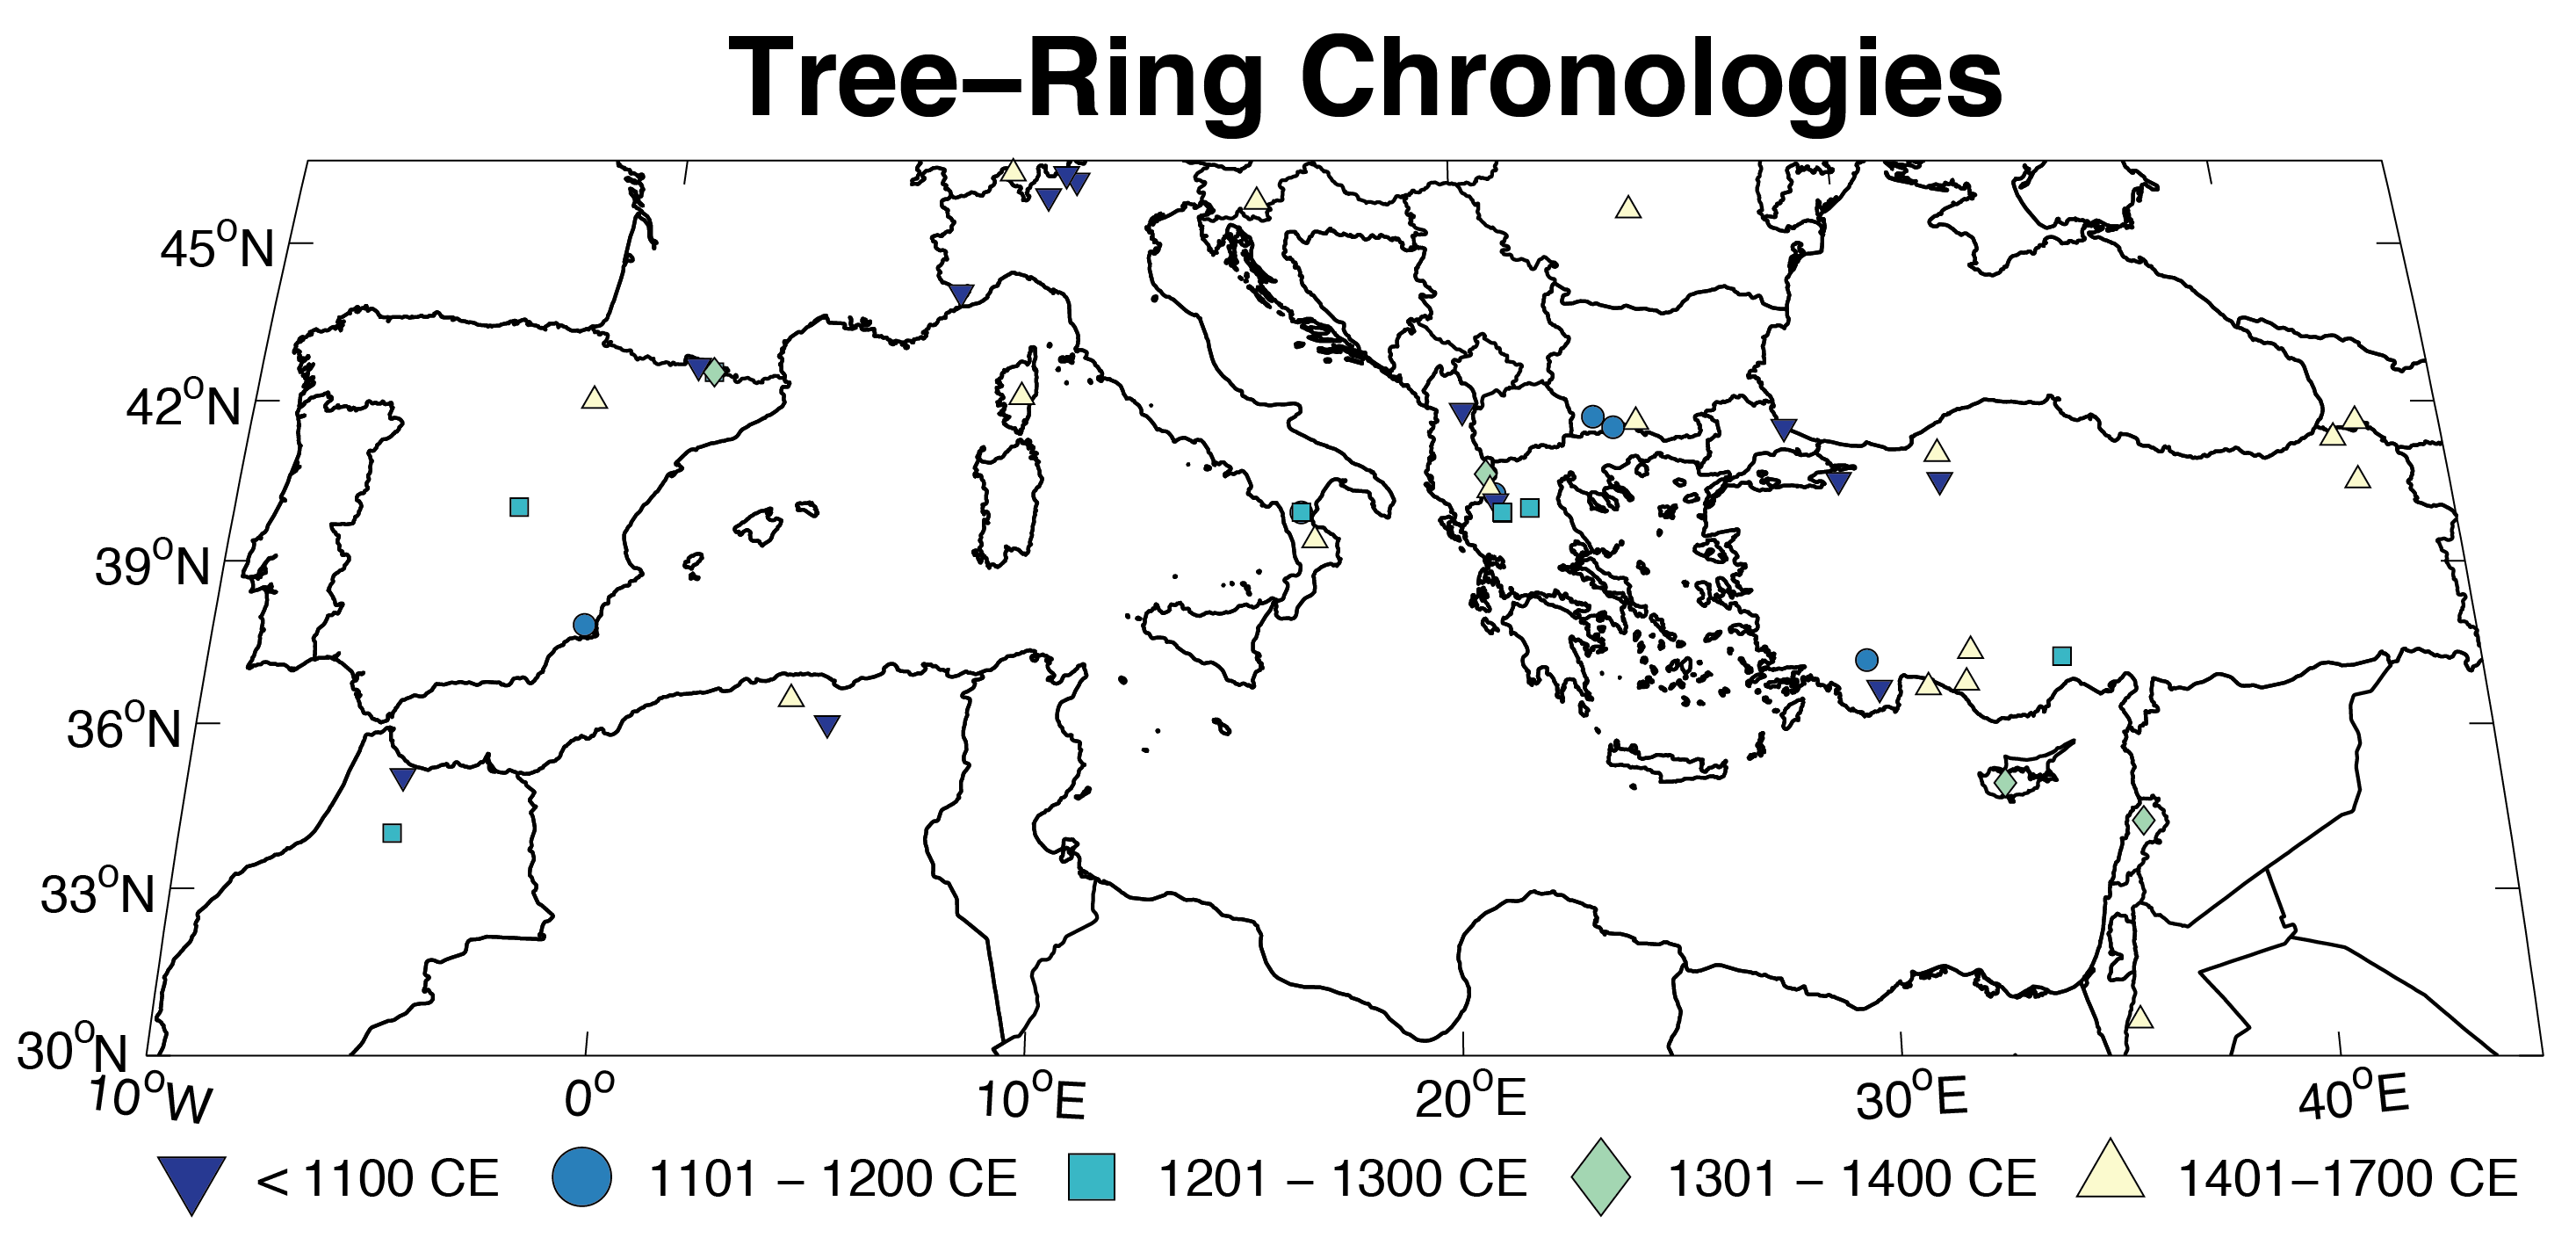
\includegraphics[width=1.0\columnwidth]{fig_01_map_sites.png}
\caption{Locations of tree-ring chronologies used for the Mediterranean portion of the Old World Drought Atlas. Colors indicate the start dates of the various chronologies.}\label{placeholder}
\end{figure}

\begin{figure}
\center
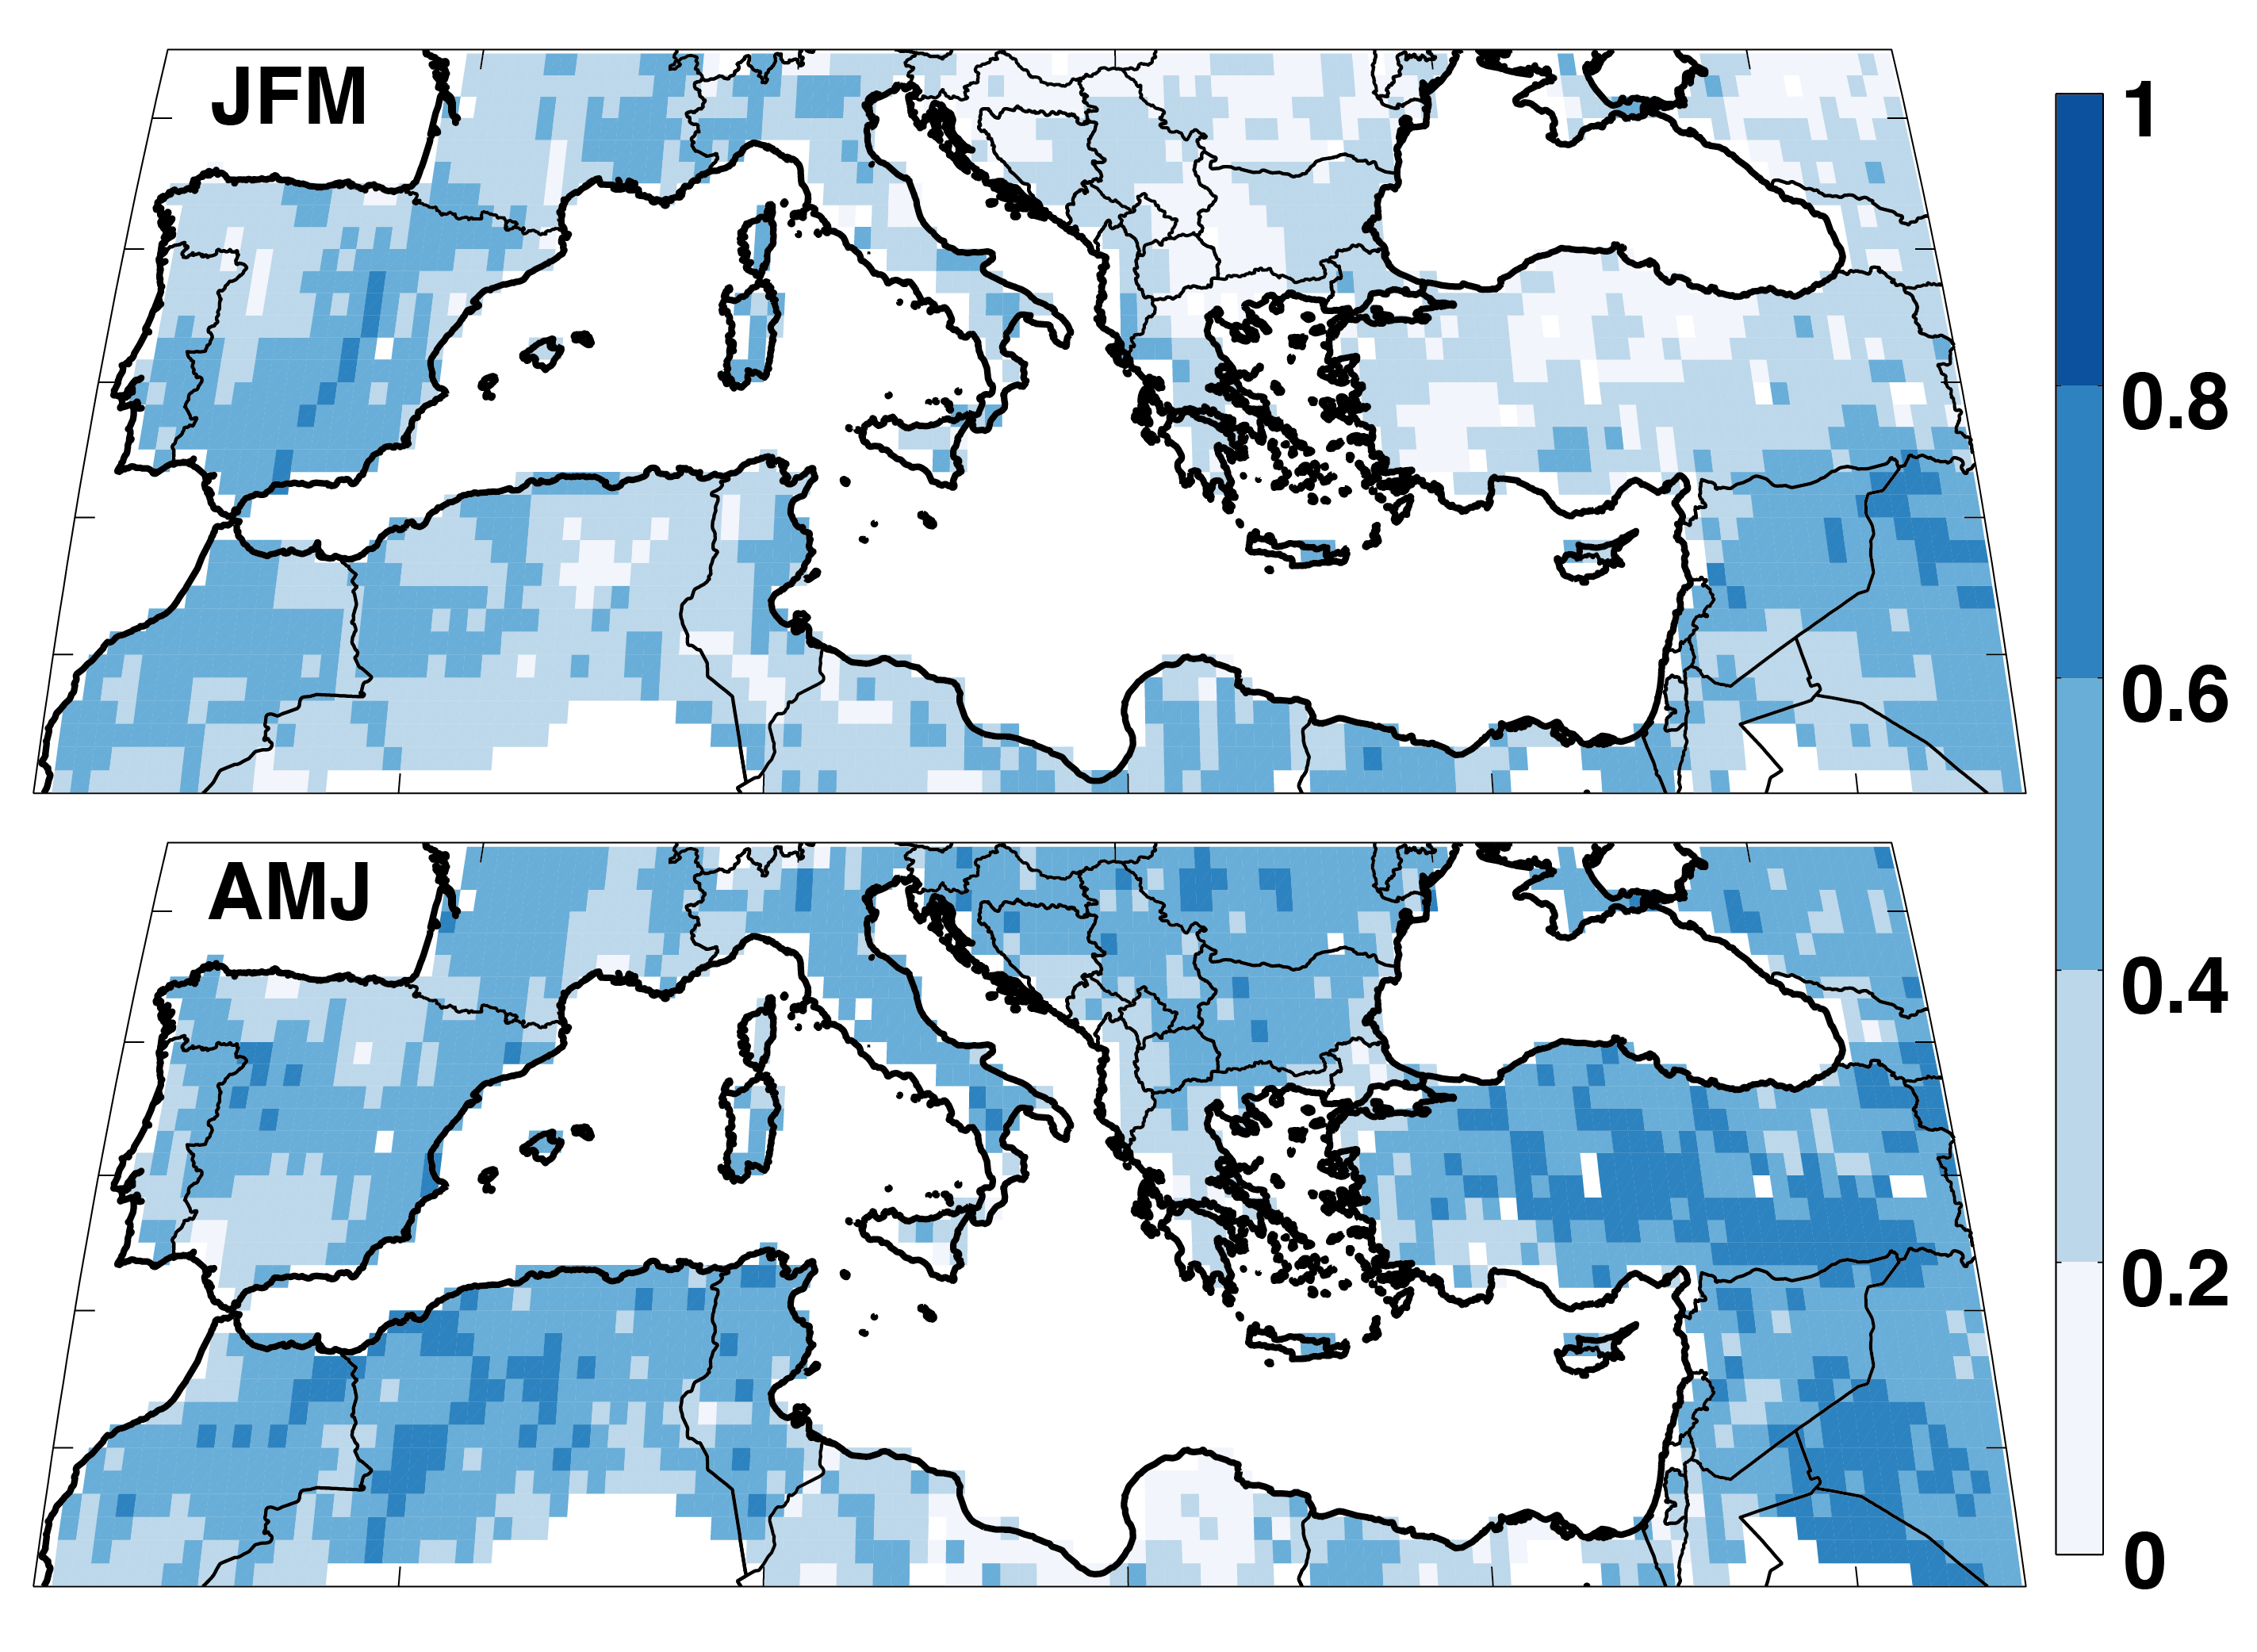
\includegraphics[width=0.9\columnwidth]{fig_02_corr_owda_prec_MED1.png}
\caption{Point-by-point Spearman's rank correlation coefficients between CRU 3.21 precipitation totals (JFM and AMJ) and OWDA summer season (JJA) scPDSI. Correlations are calculated over the period 1950--2012 CE.}\label{placeholder}
\end{figure}

\begin{figure}
\center
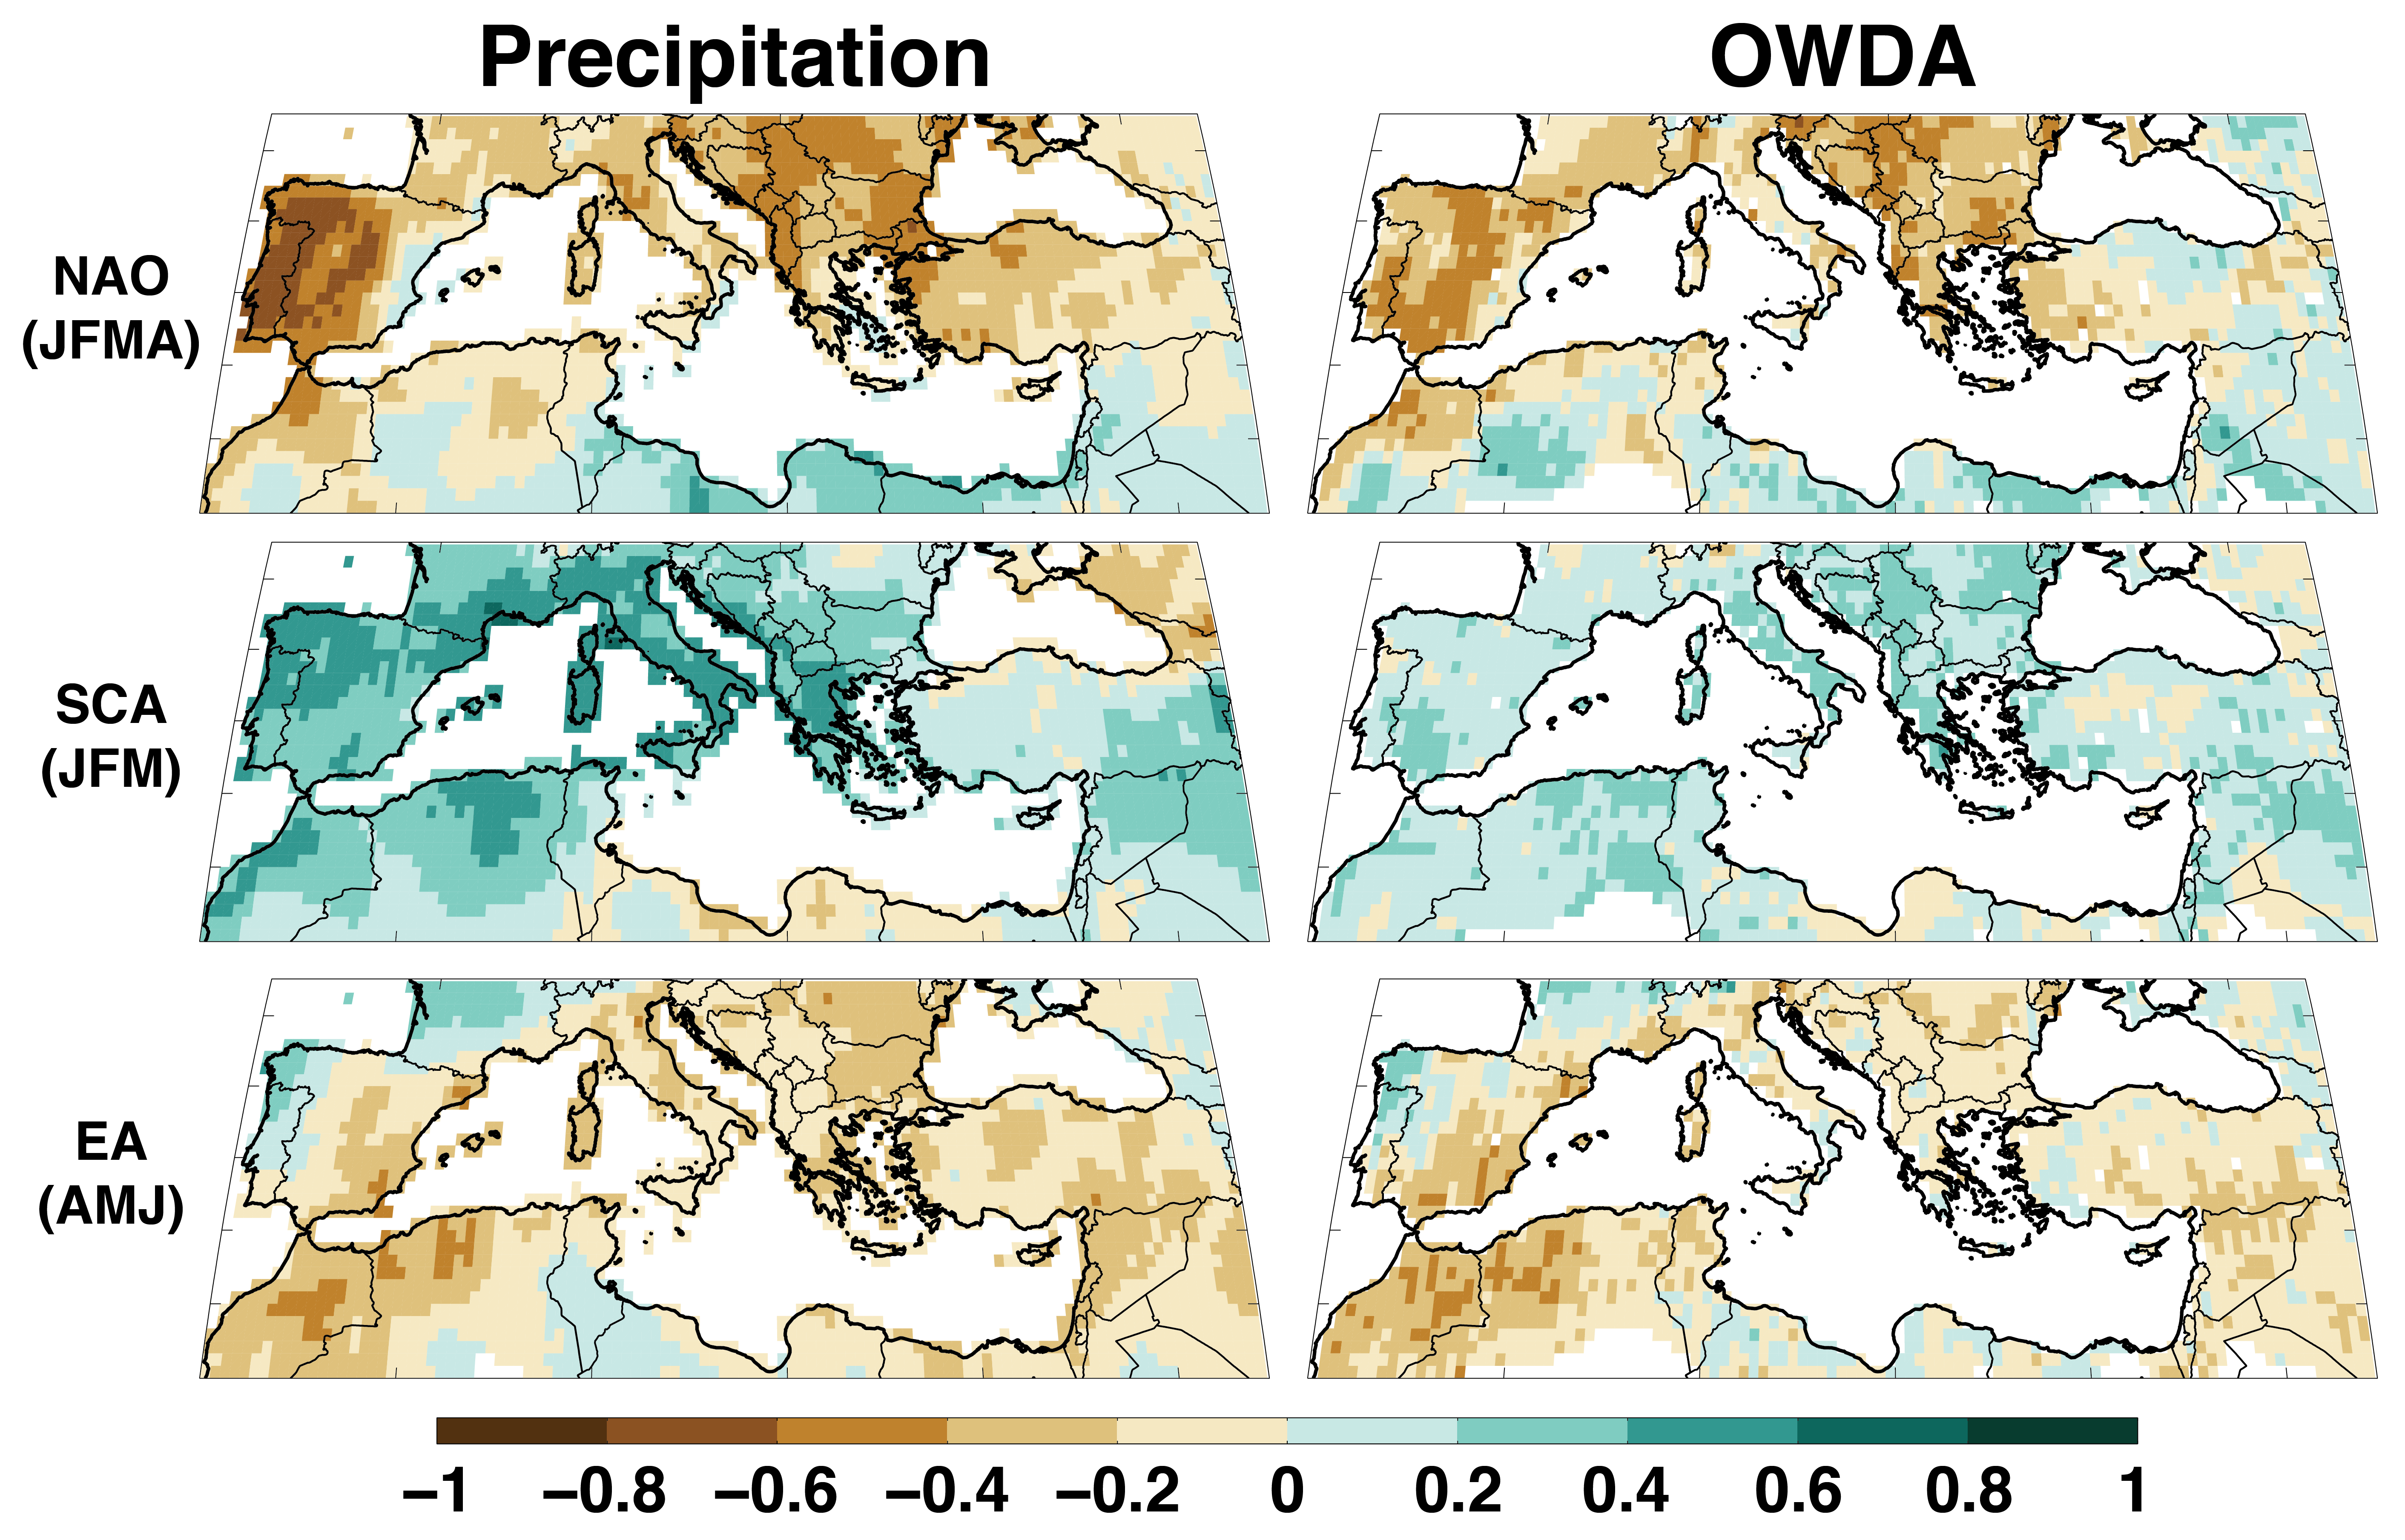
\includegraphics[width=1.0\columnwidth]{fig_03_teleconn_corr_MED1.png}
\caption{Spearman's rank correlation coefficients between the teleconnection indices (NAO, SCA, EA) and simultaneous season CRU 3.21 precipitation totals (left column) and OWDA summer season scPDSI (right column). Correlations are calculated over the period 1950--2012 CE.}\label{placeholder}
\end{figure}

\begin{figure}
\center
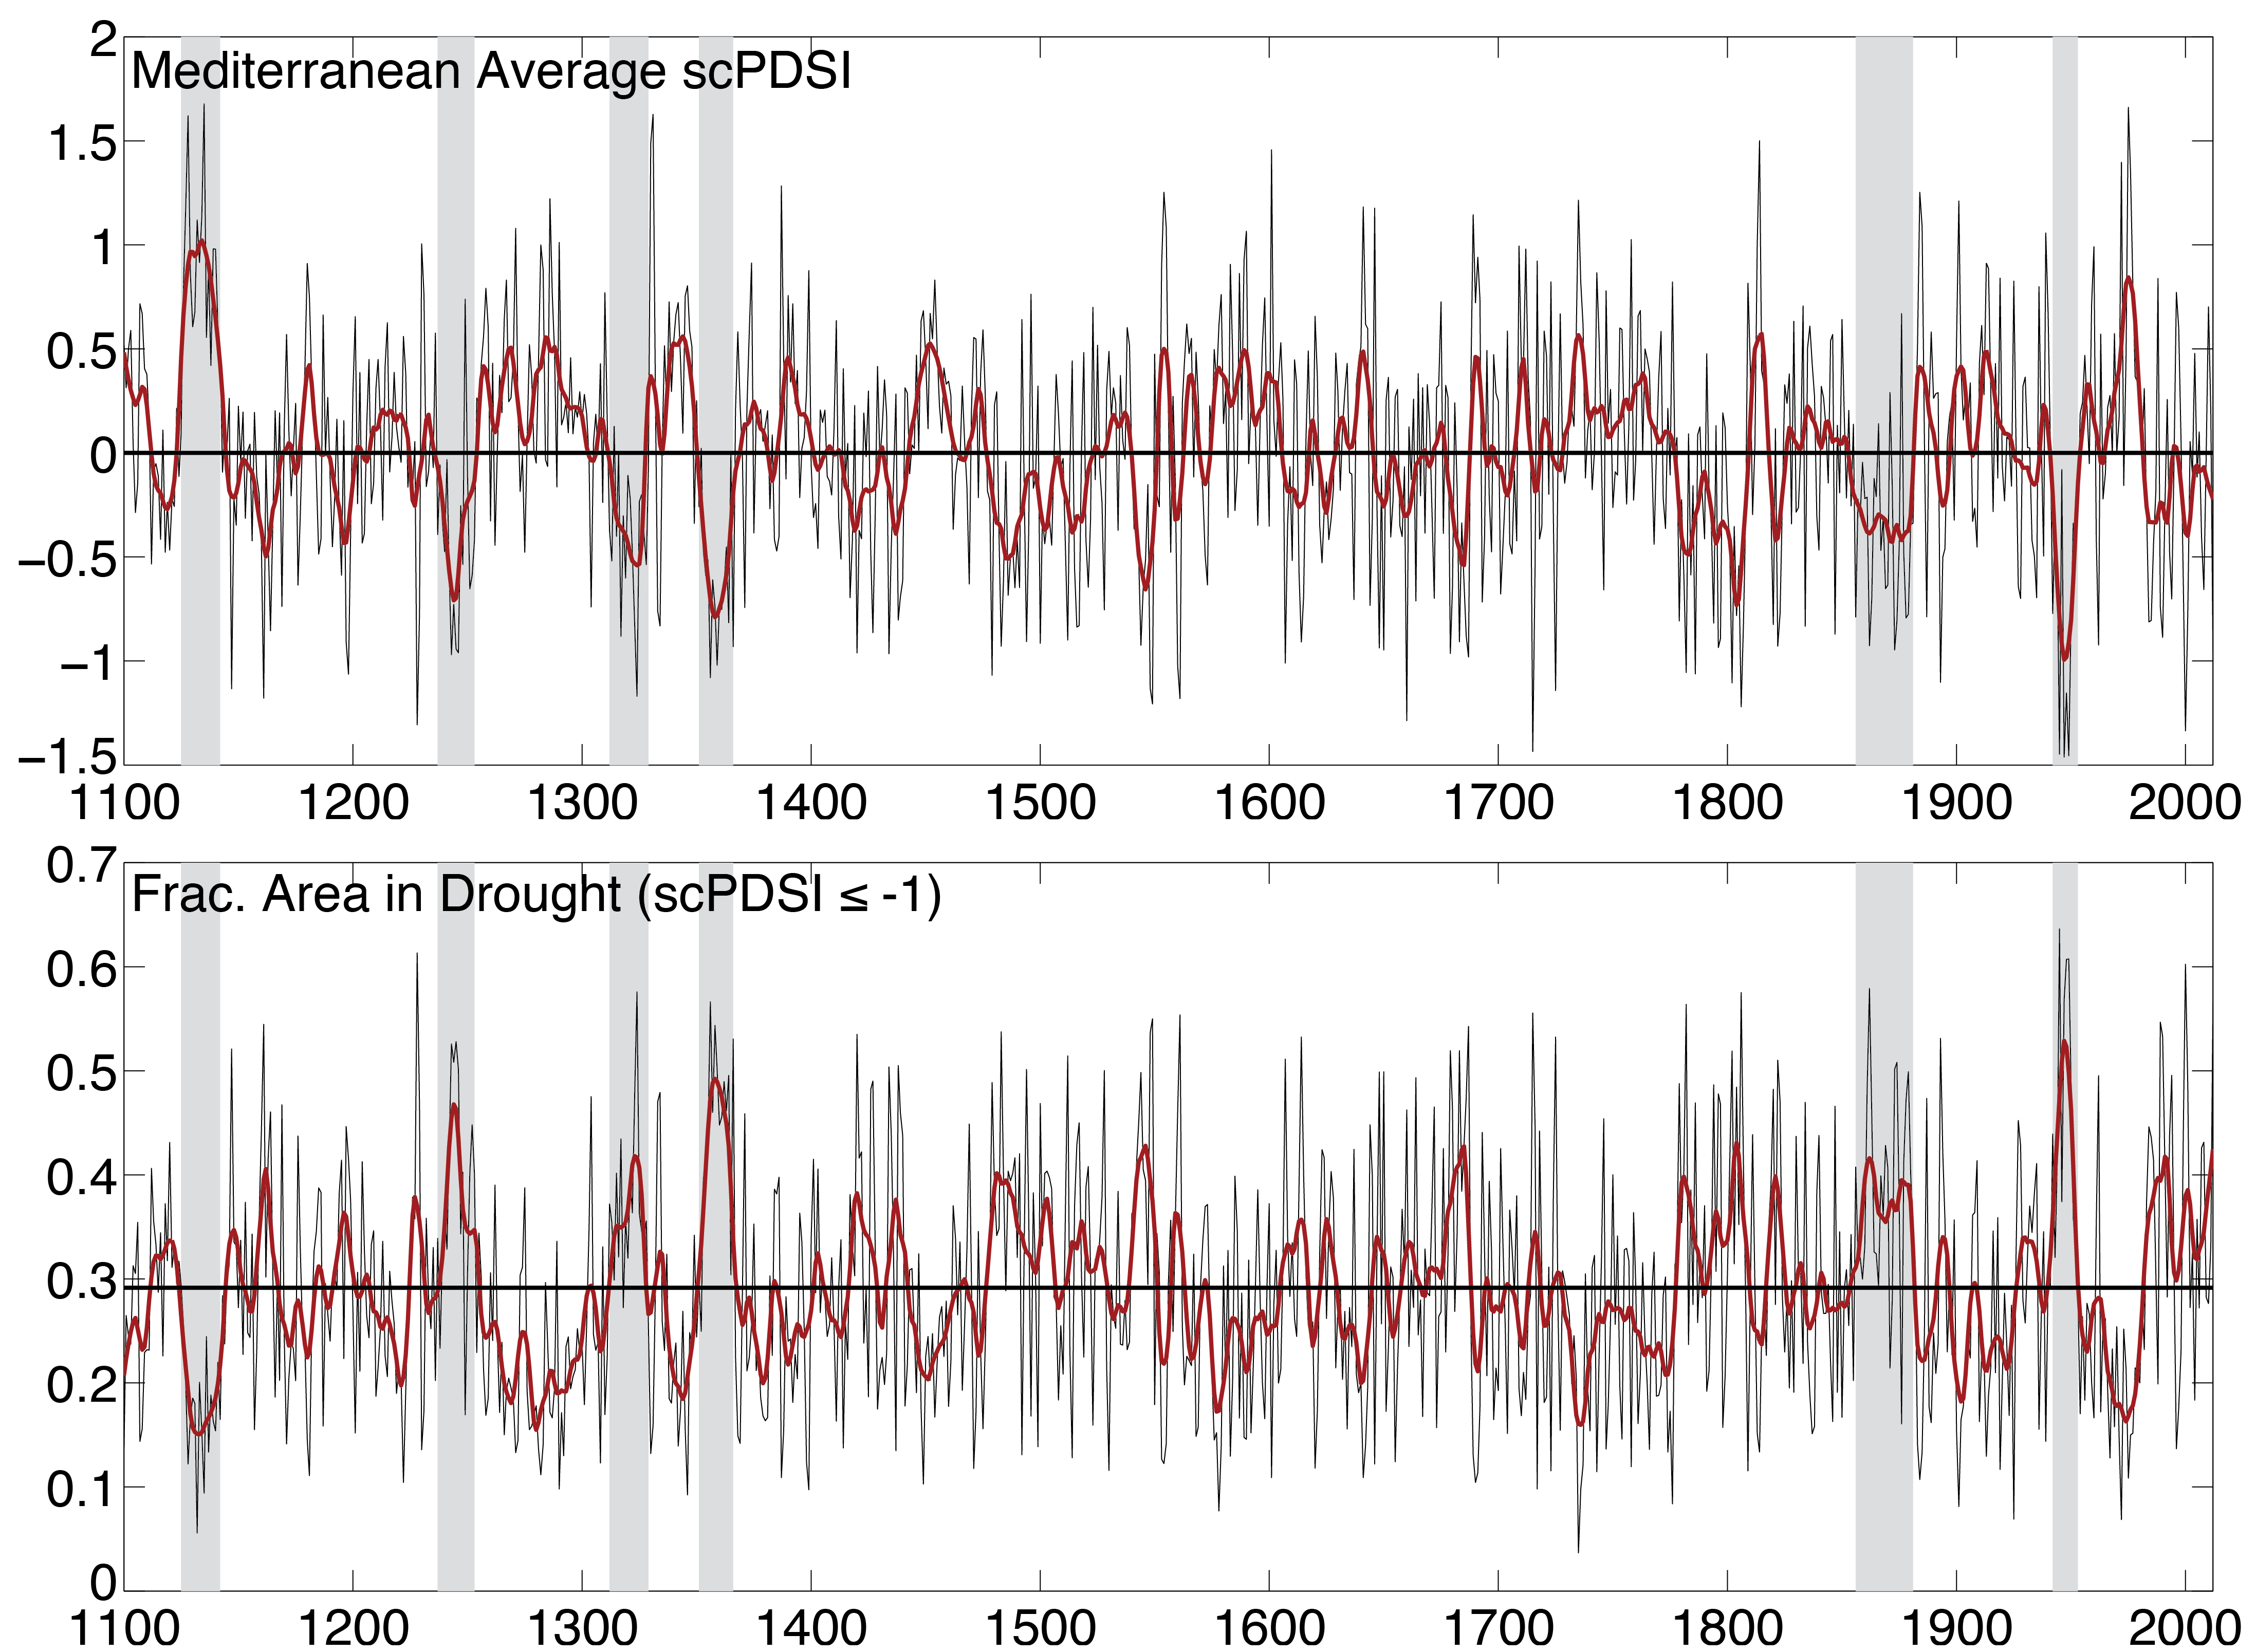
\includegraphics[width=1.0\columnwidth]{fig_04_ave_area_pdsi_MED1.png}
\caption{Area average scPDSI for the entire Mediterranean domain in the OWDA (30\textsuperscript{o}N--47\textsuperscript{o}N, 10\textsuperscript{o}W--45\textsuperscript{o}E) (top) and percent land area in drought (scPDSI$\le-1$) (bottom) from 1100--2012 CE. Red curves are smoothed versions of the time series using a 10-year loess smooth. The horizontal line in the lower panel is the long-term average fractional area in drought from 1100--2012 CE (29\%). Highlighted in grey are several example periods of persistent pan-basin drought and pluvial events (see Figure 5).}\label{placeholder}
\end{figure}

\begin{figure}
\center
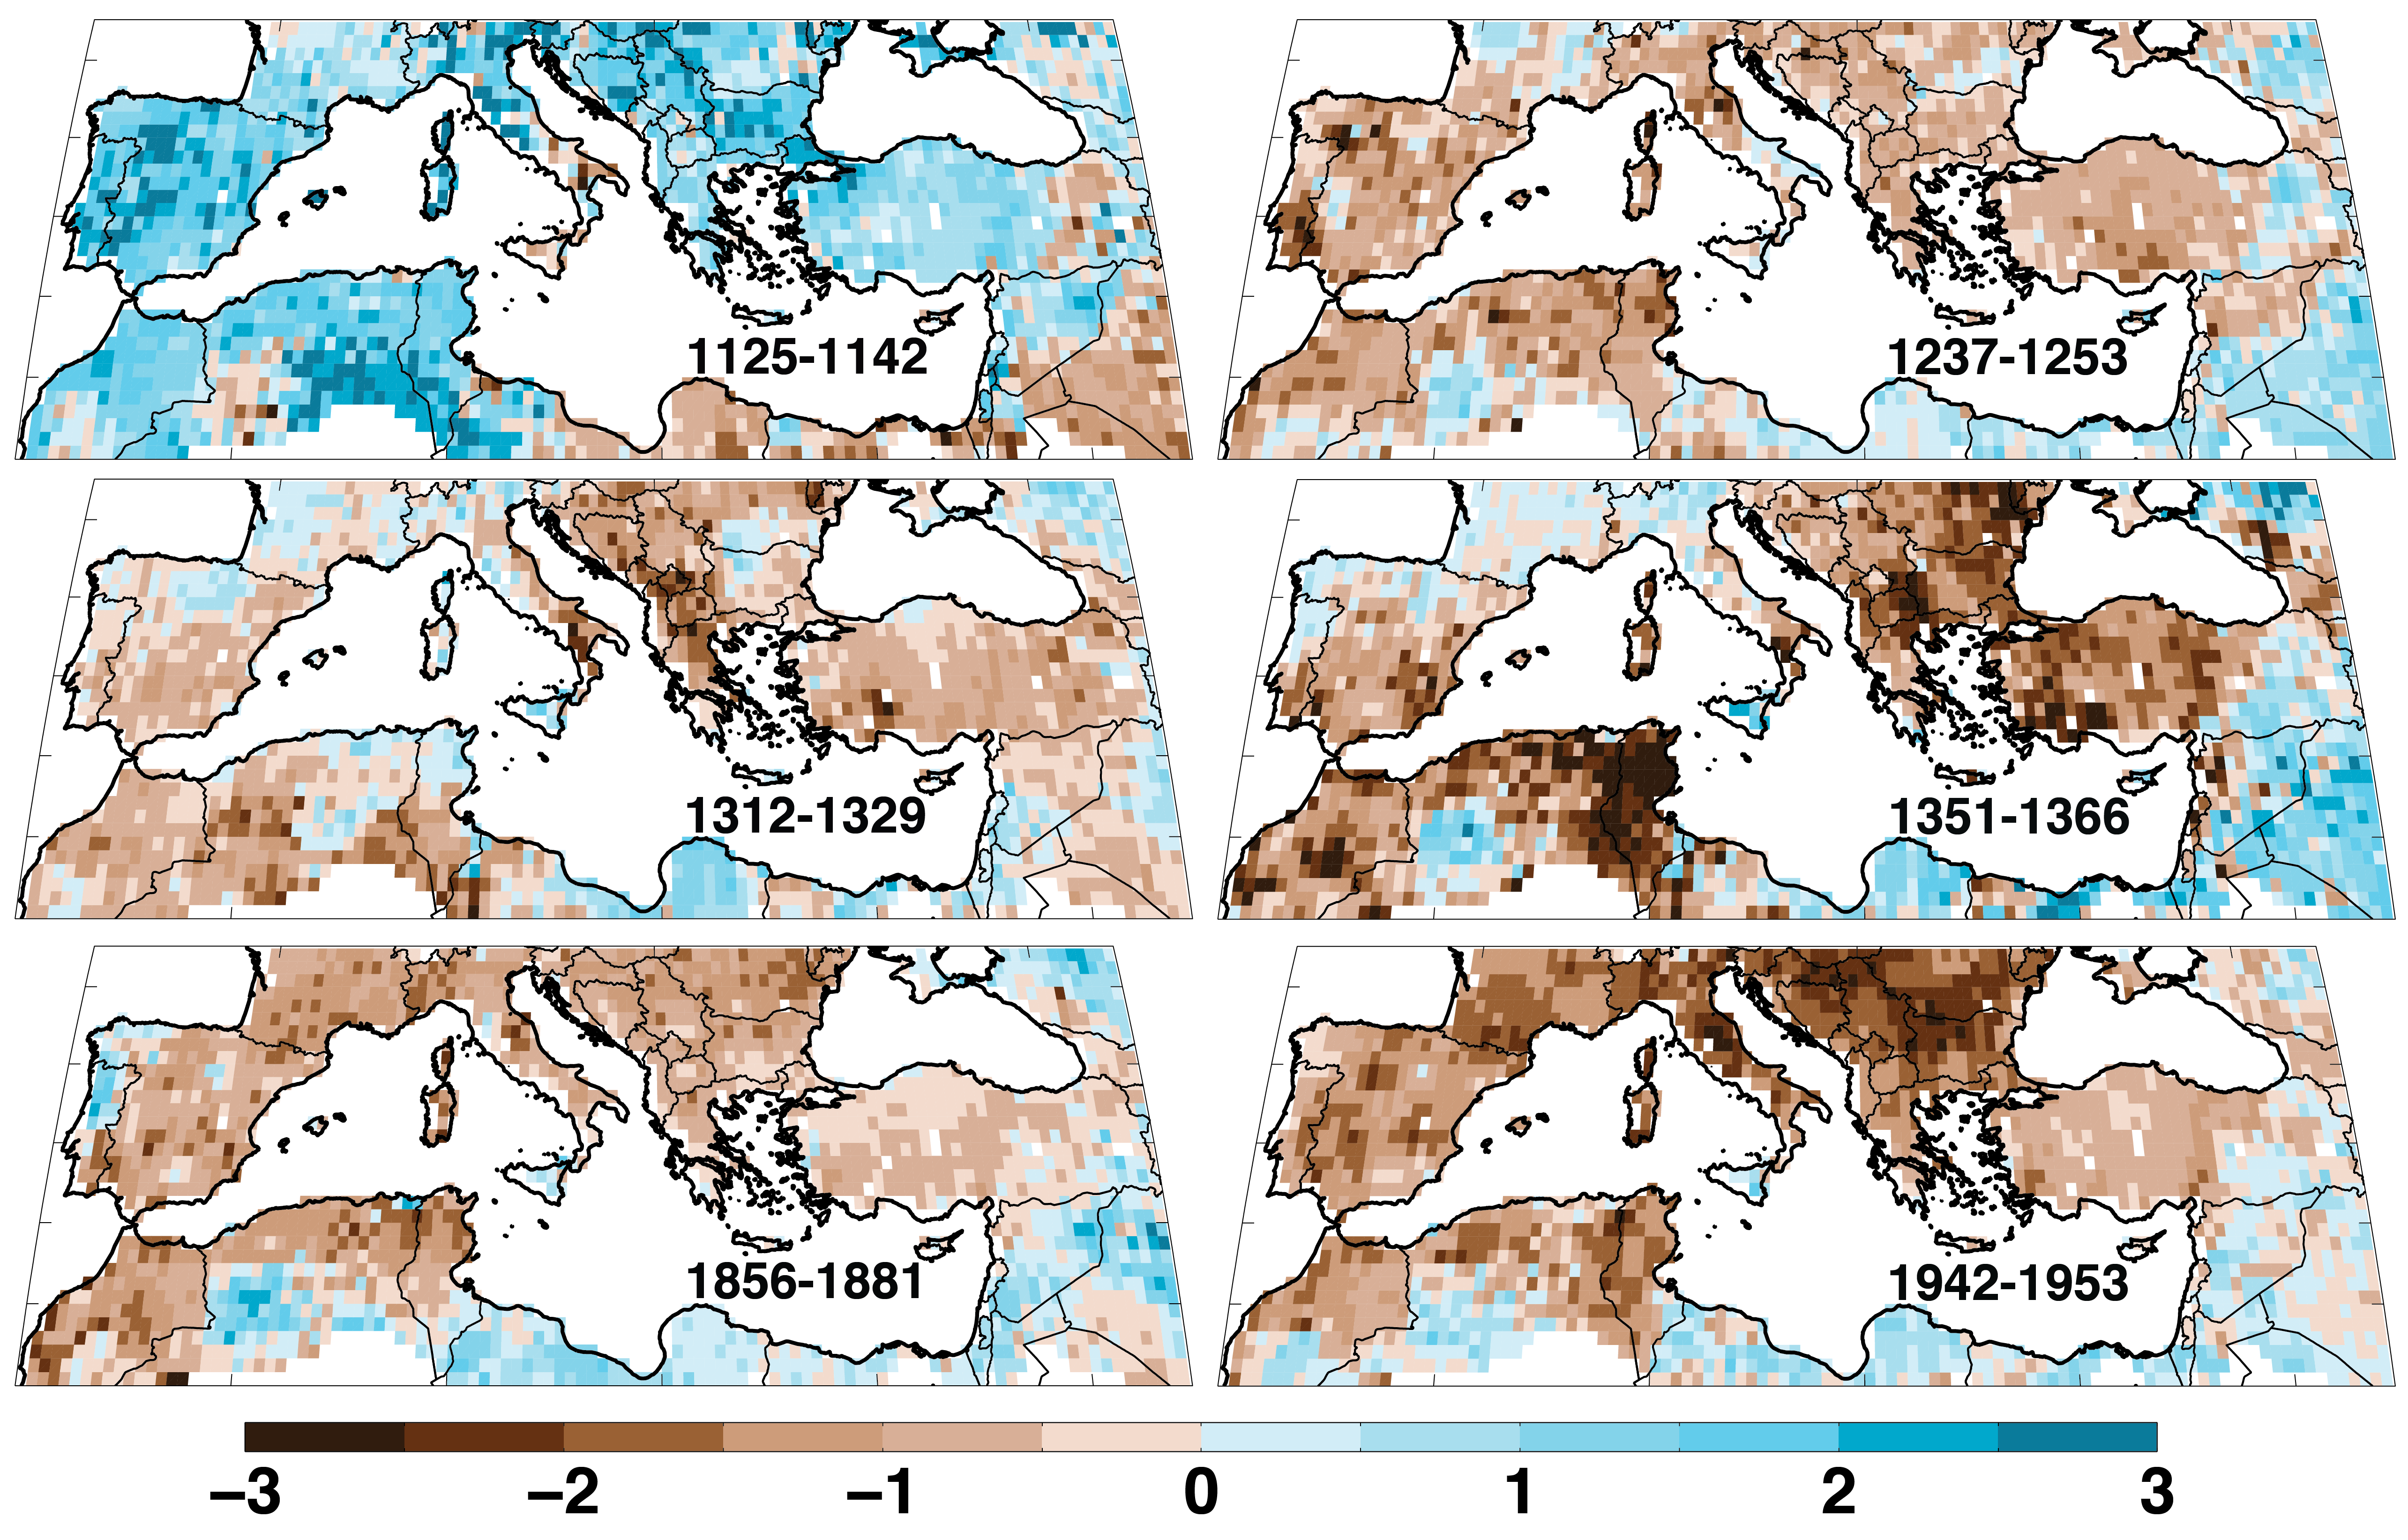
\includegraphics[width=1.0\columnwidth]{fig_05_drght_pluv_events.png}
\caption{Multi-year average scPDSI for different pan-basin drought and pluvial events in the OWDA.}\label{placeholder}
\end{figure}

\begin{figure}
\center
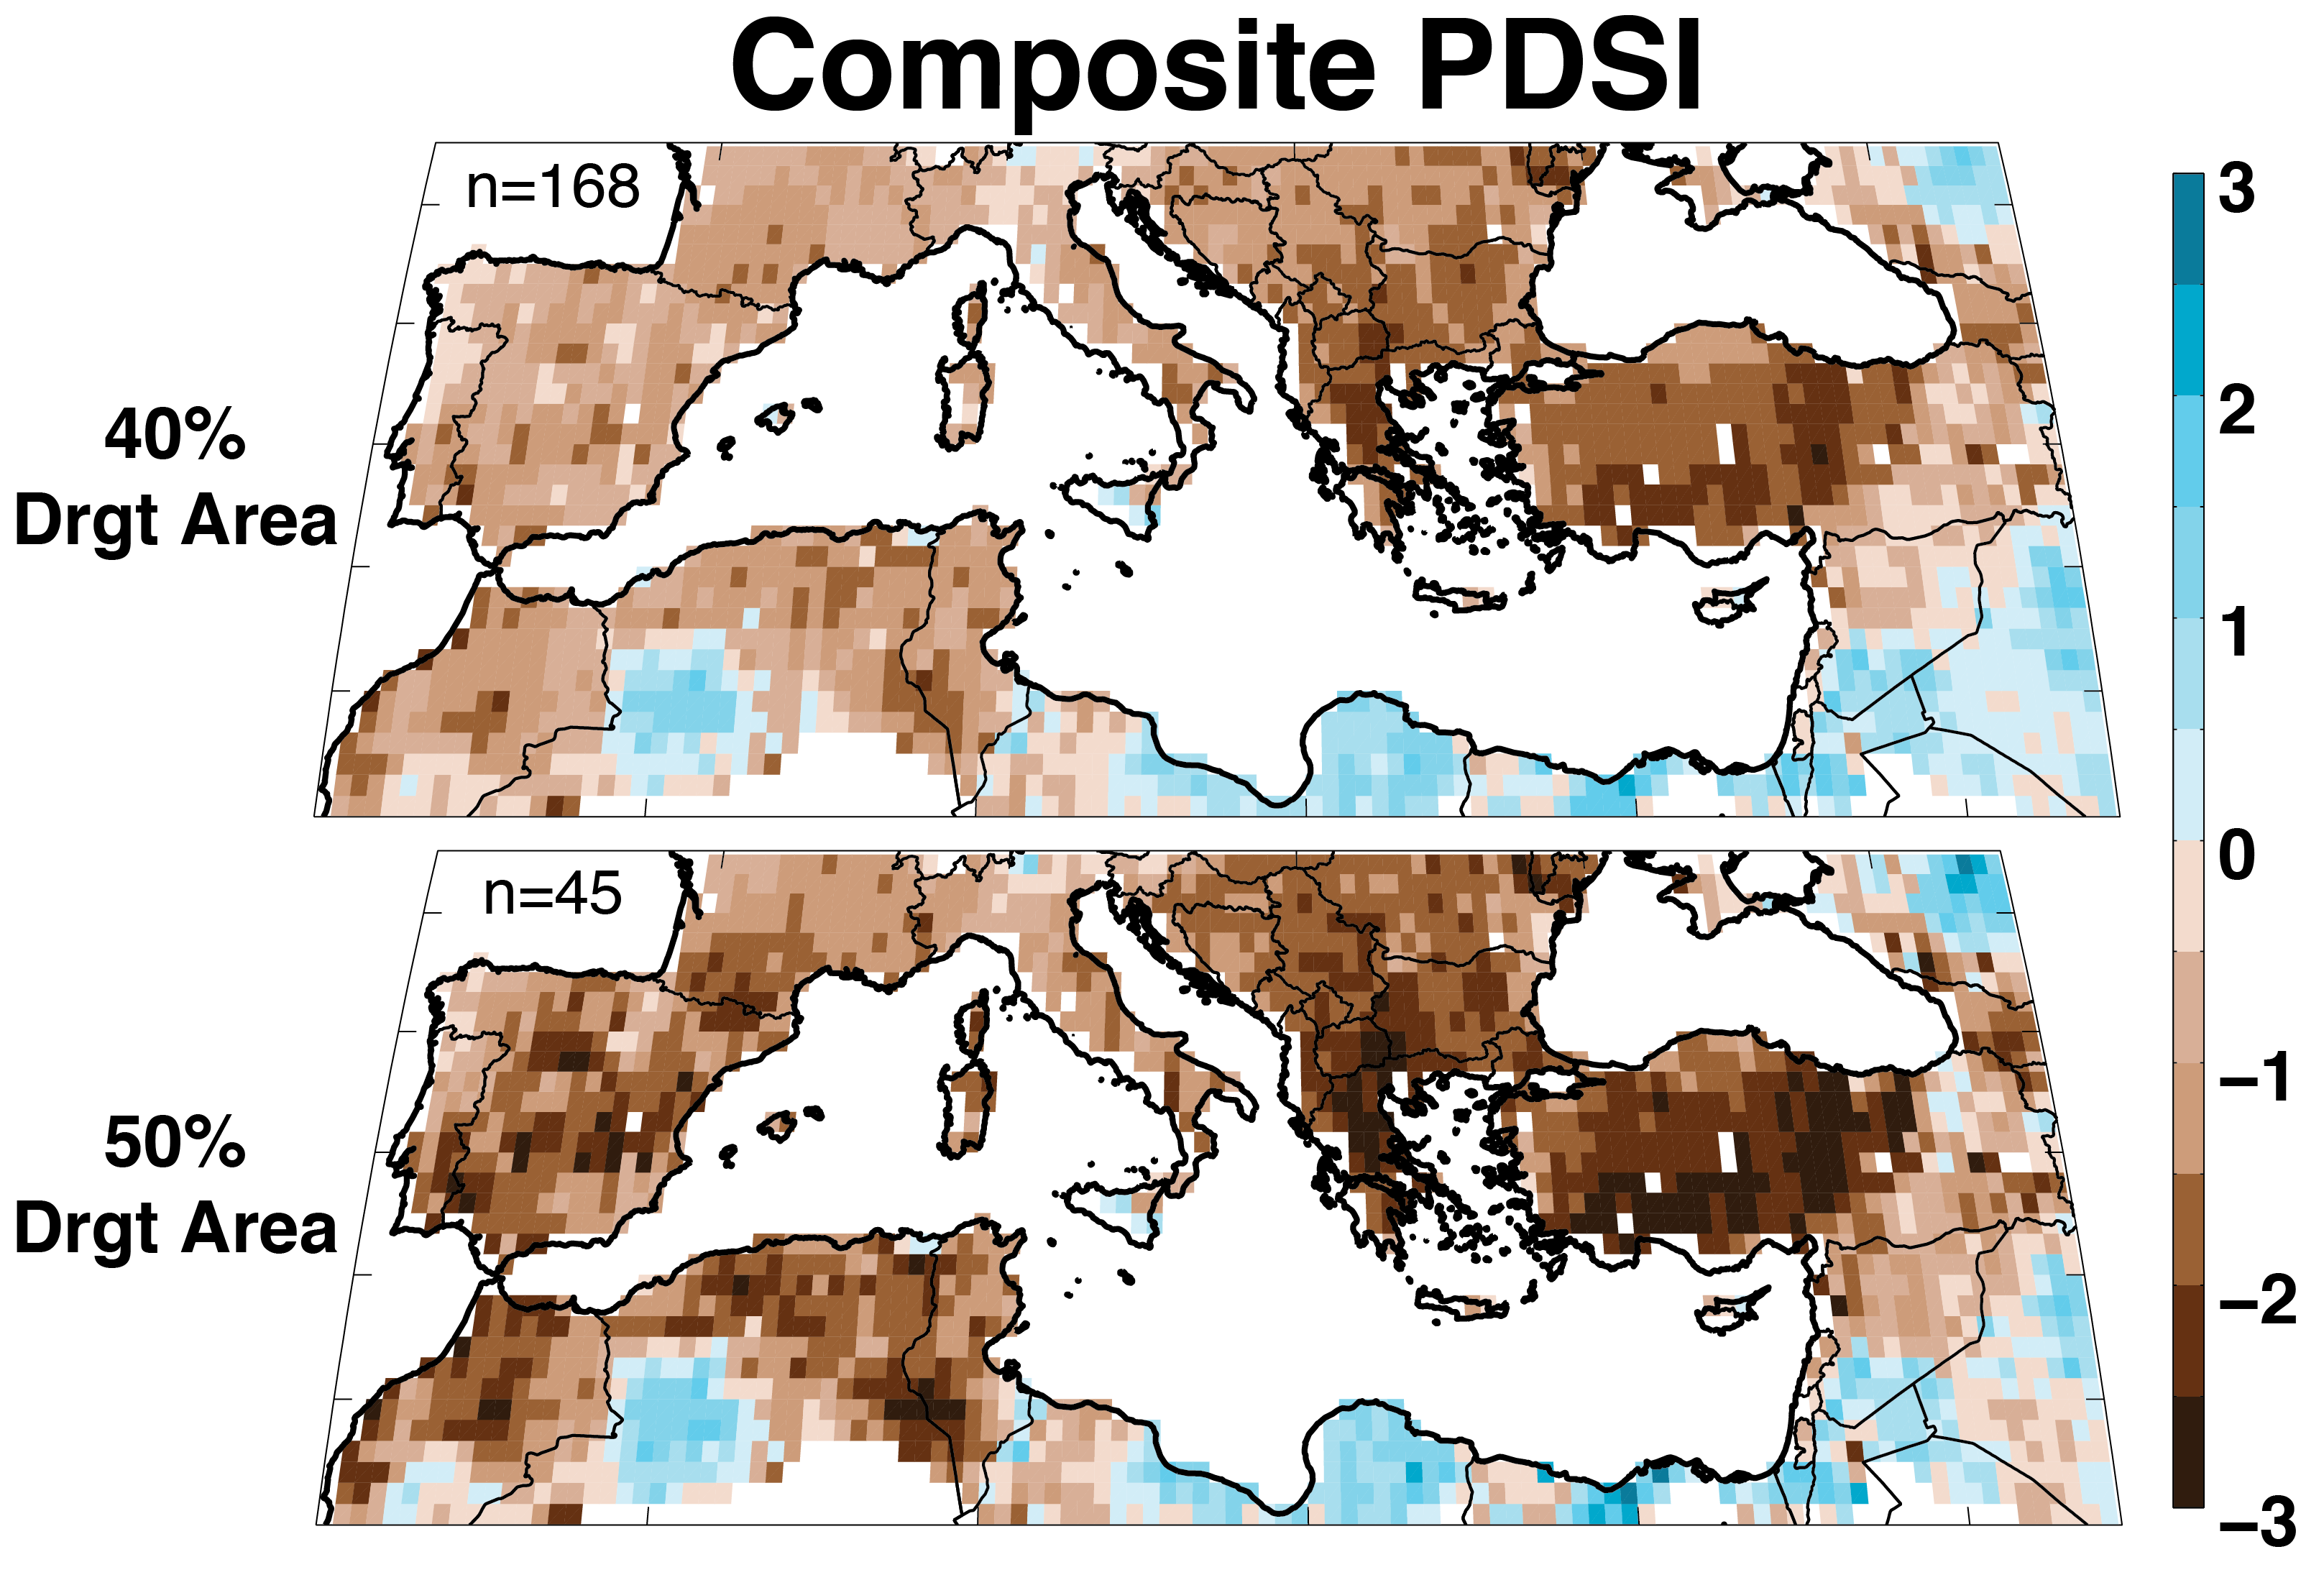
\includegraphics[width=0.9\columnwidth]{fig_06_pdsi_40_50_composite.png}
\caption{Composite average of Mediterranean drought events in the OWDA with a drought area (scPDSI$\le-1$) exceeding 40\% ($n=$168 years) and 50\% ($n=$45 years) of the total land area in the Mediterranean domain.}\label{placeholder}
\end{figure}

\begin{figure}
\center
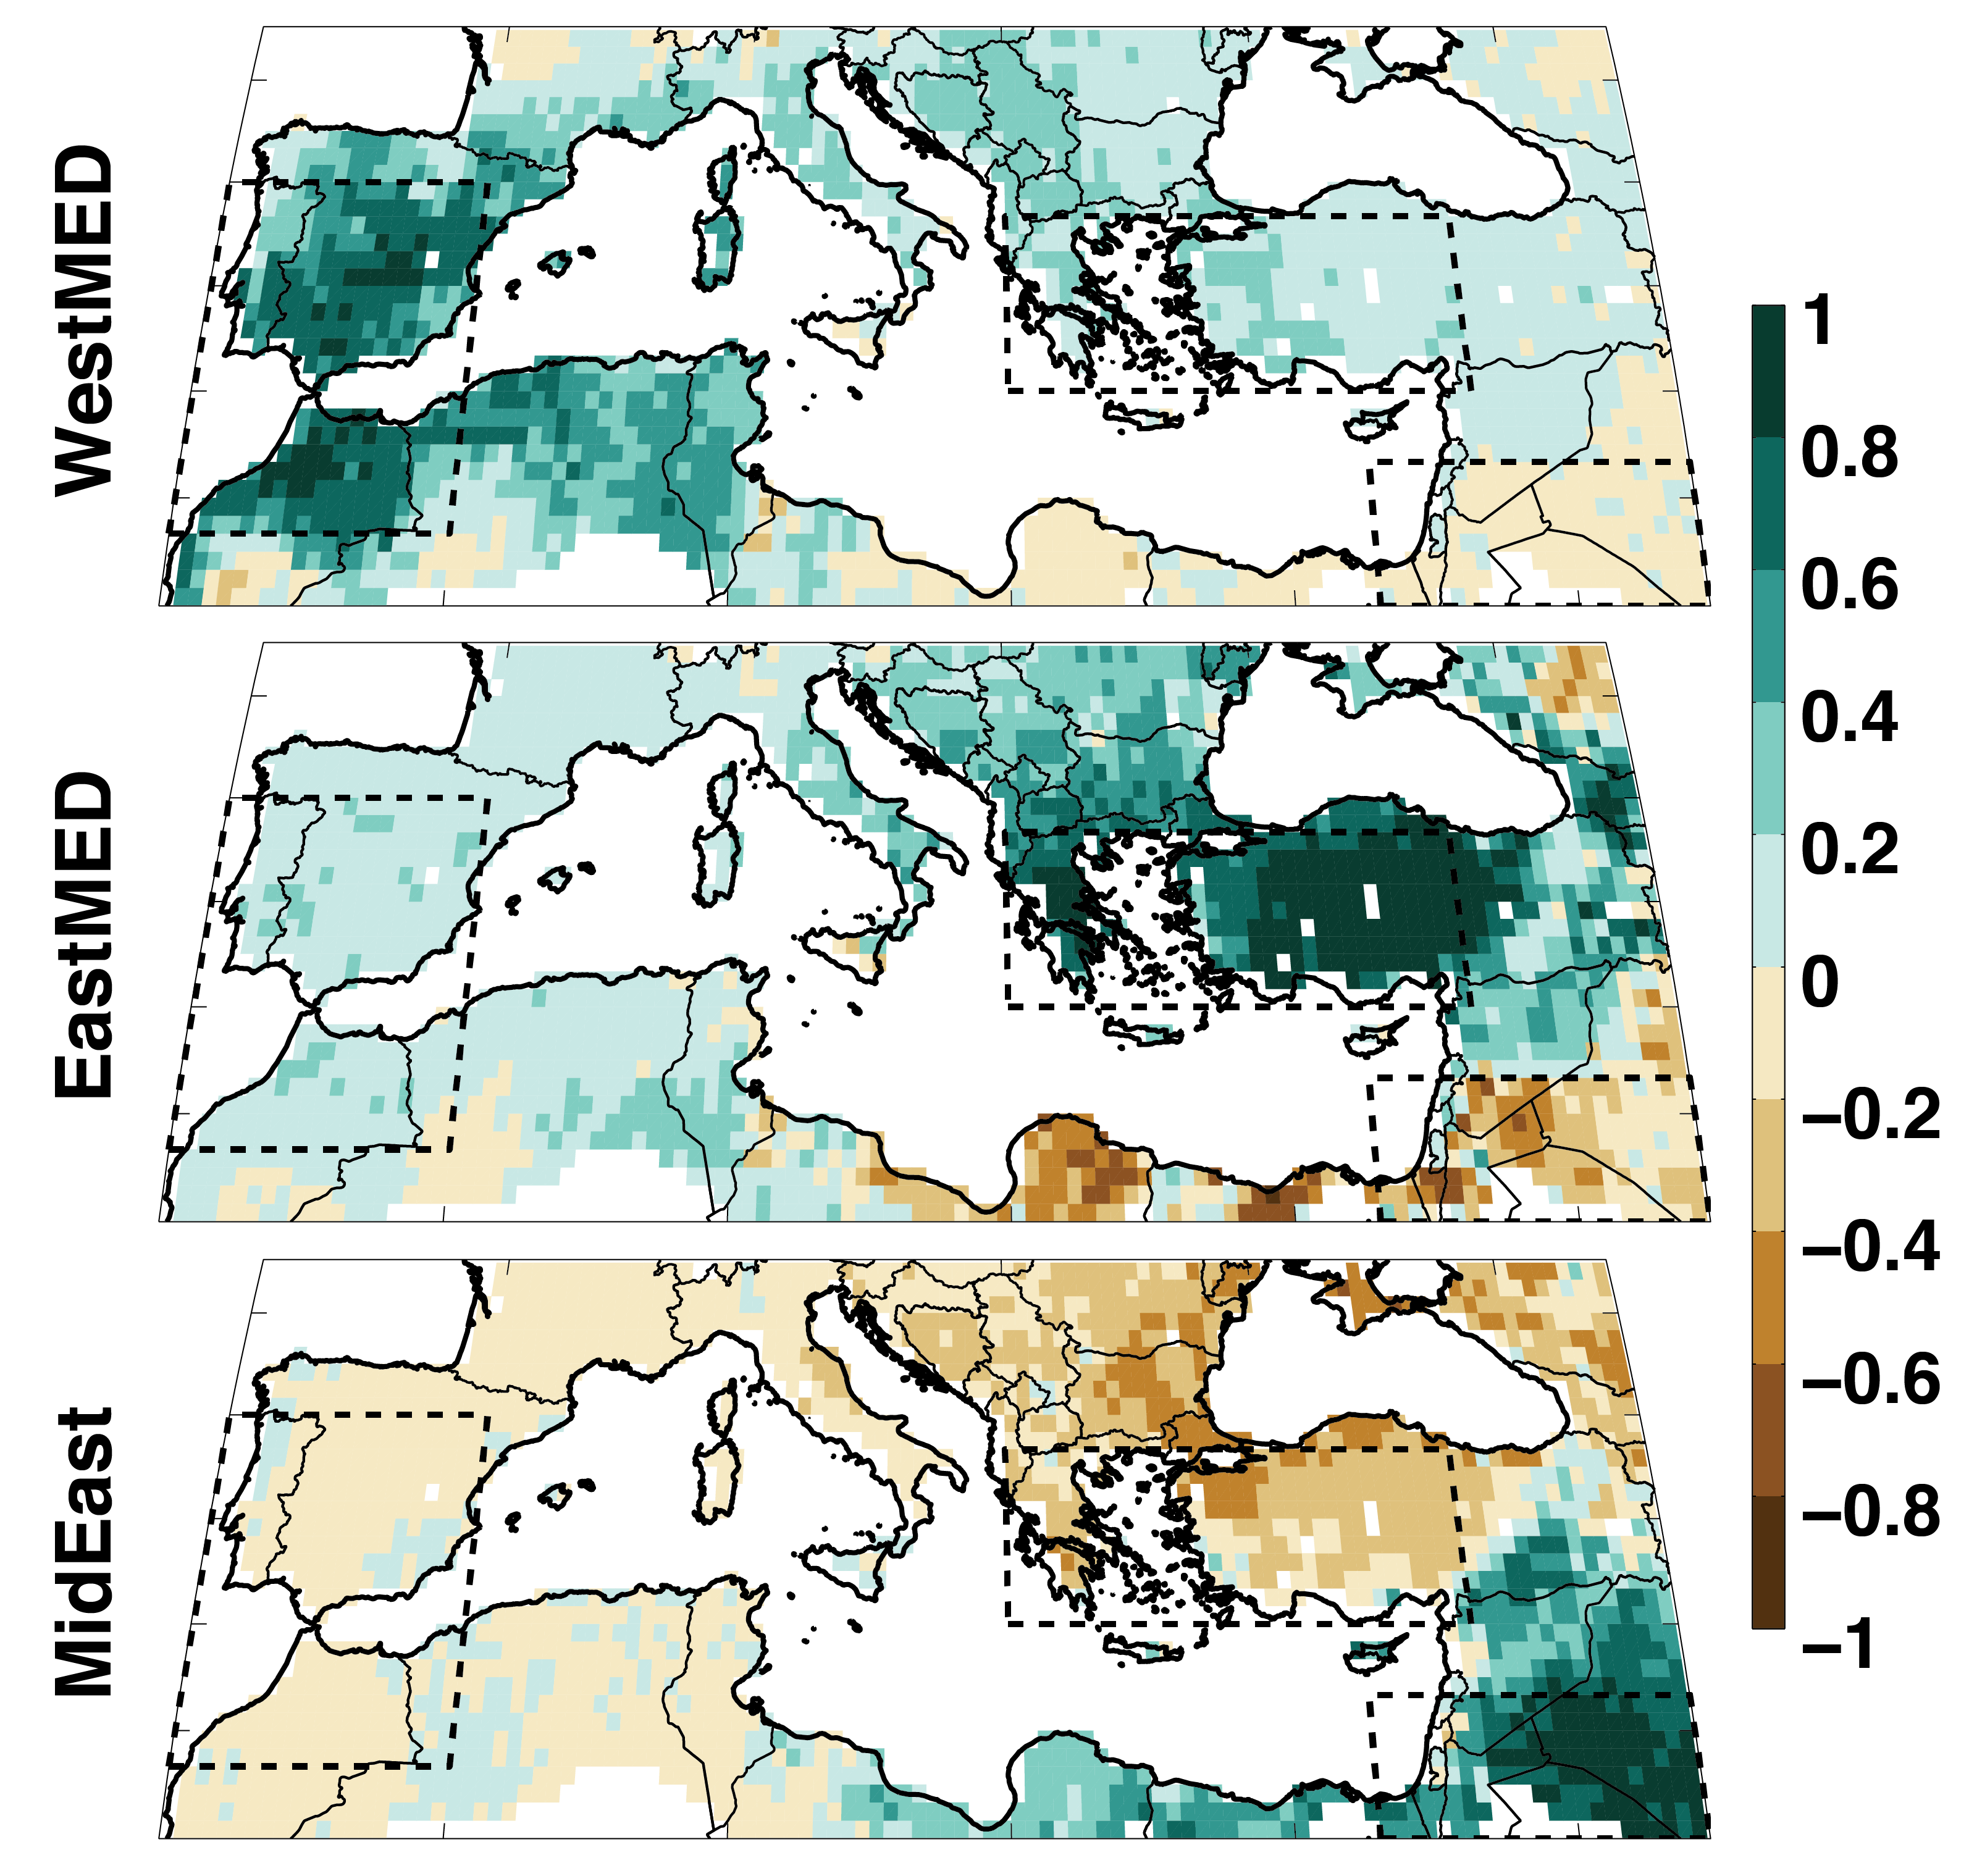
\includegraphics[width=0.9\columnwidth]{fig_07_east_west_mideast_corrmap.png}
\caption{Point-by-point Spearman's rank correlations (1100--2012) between OWDA scPDSI and the Western Mediterranean (WestMED; 32\textsuperscript{o}N--42\textsuperscript{o}N, 10\textsuperscript{o}W--0\textsuperscript{o}), Eastern Mediterranean (EastMED; 36\textsuperscript{o}N--41\textsuperscript{o}N, 20\textsuperscript{o}E--37\textsuperscript{o}E), and Middle East (MidEast; 30\textsuperscript{o}N--34\textsuperscript{o}N, 33\textsuperscript{o}E--47\textsuperscript{o}E) regional average scPDSI time series.}\label{placeholder}
\end{figure}

\begin{figure}
\center
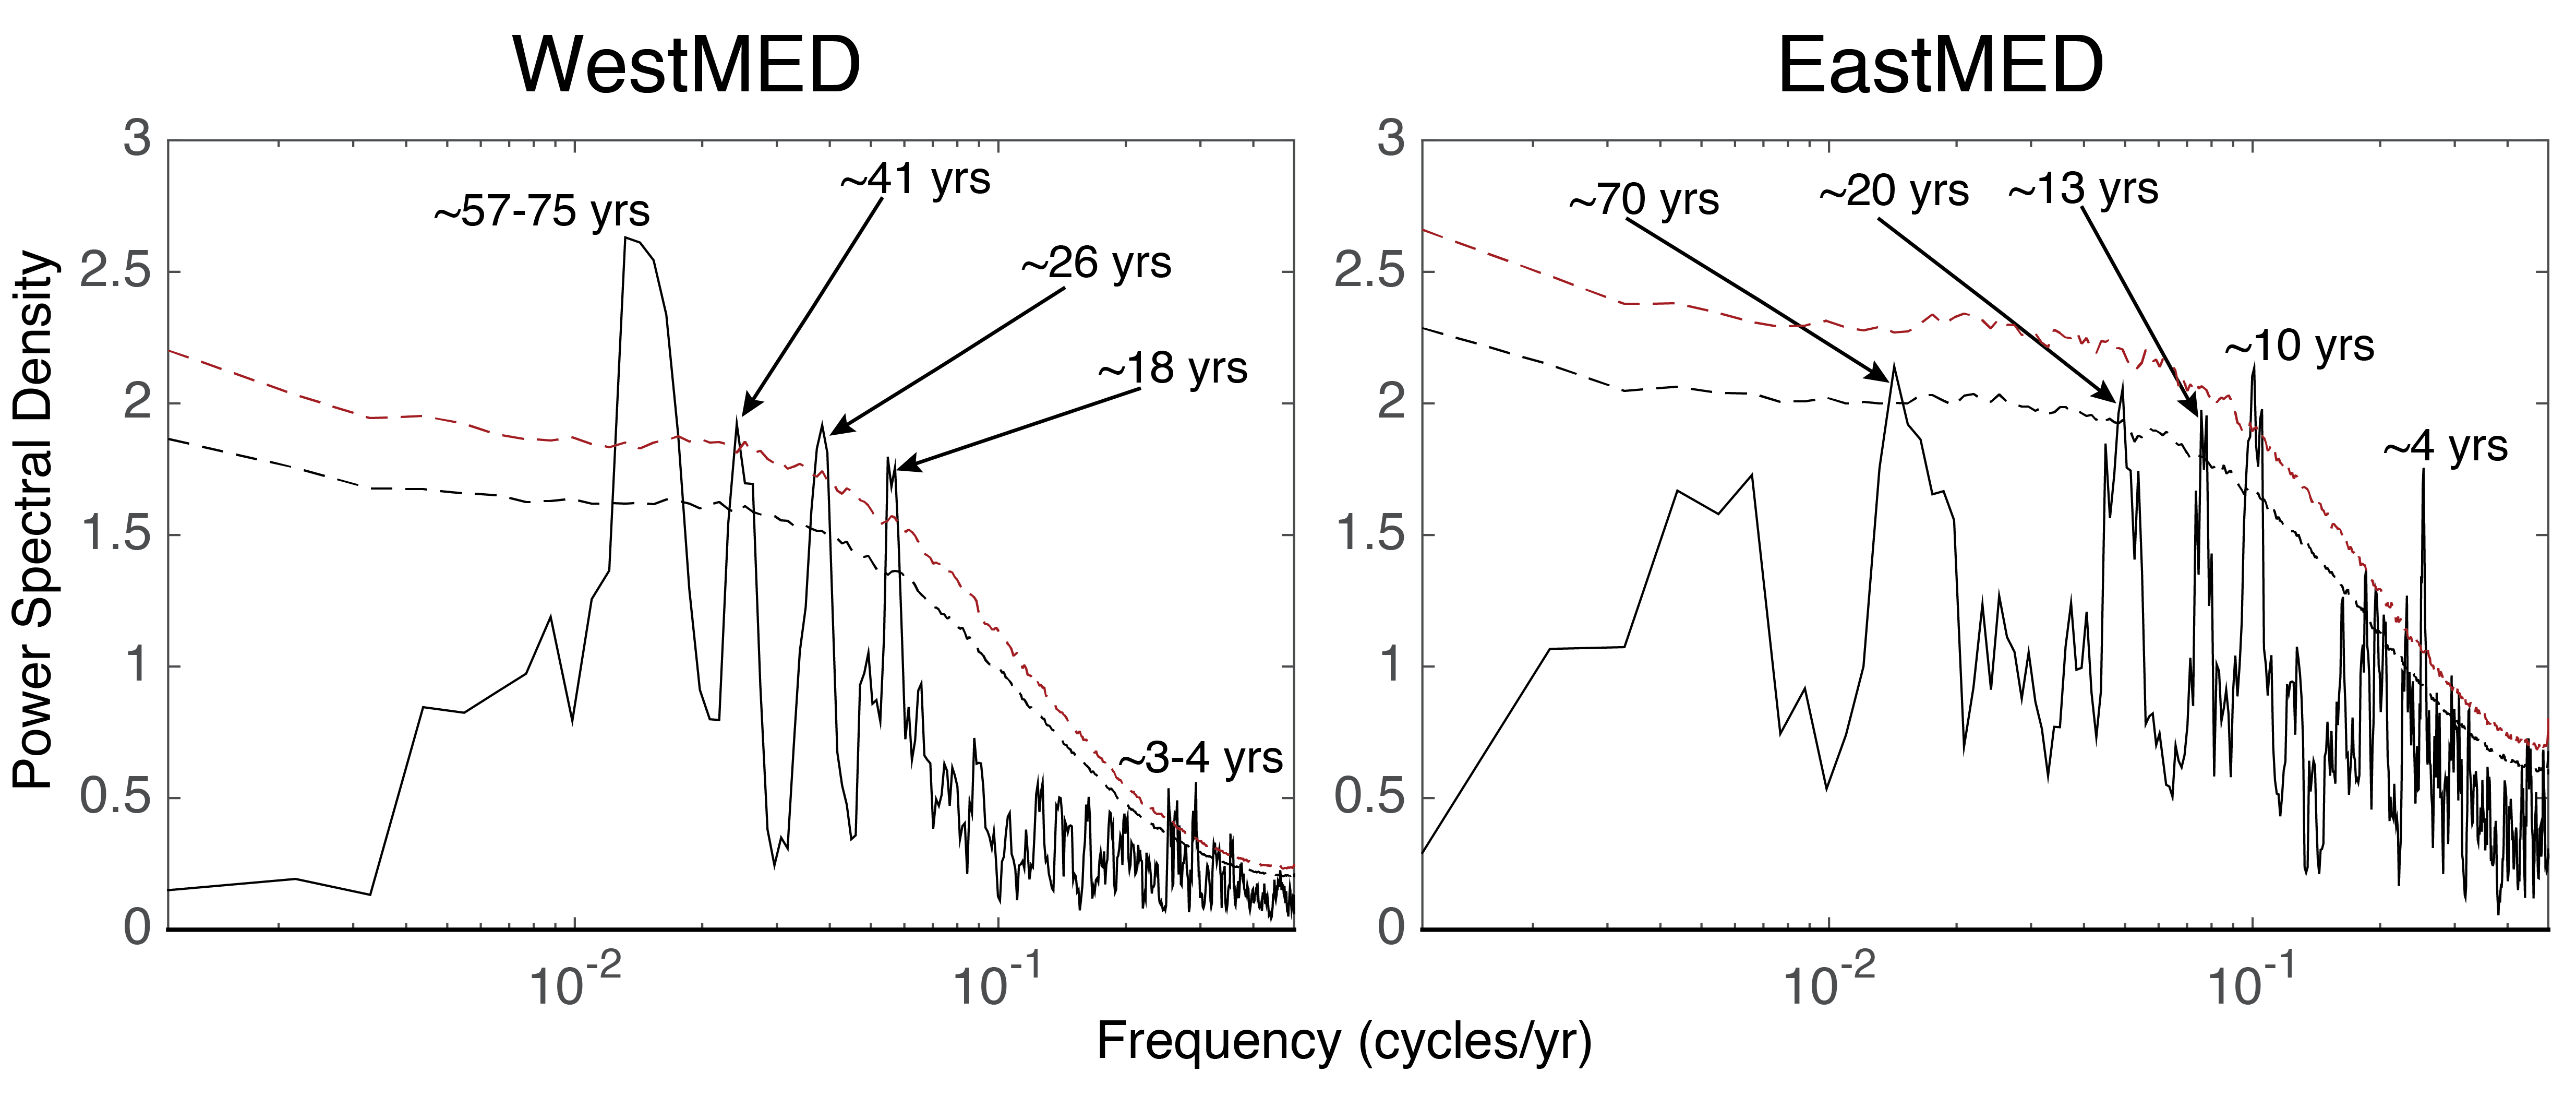
\includegraphics[width=1.0\columnwidth]{fig_08_eastwest_mtm_spectra.png}
\caption{Power spectral density (Multi-taper Method, 3 tapers) for the WestMED and EastMED regional average scPDSI series. Red and black dashed lines are the 95\textsuperscript{th} and 90\textsuperscript{th} confidence limits, respectively, estimated from 10,000 AR(1) series generated from the original time series.}\label{placeholder}
\end{figure}

\begin{figure}
\center
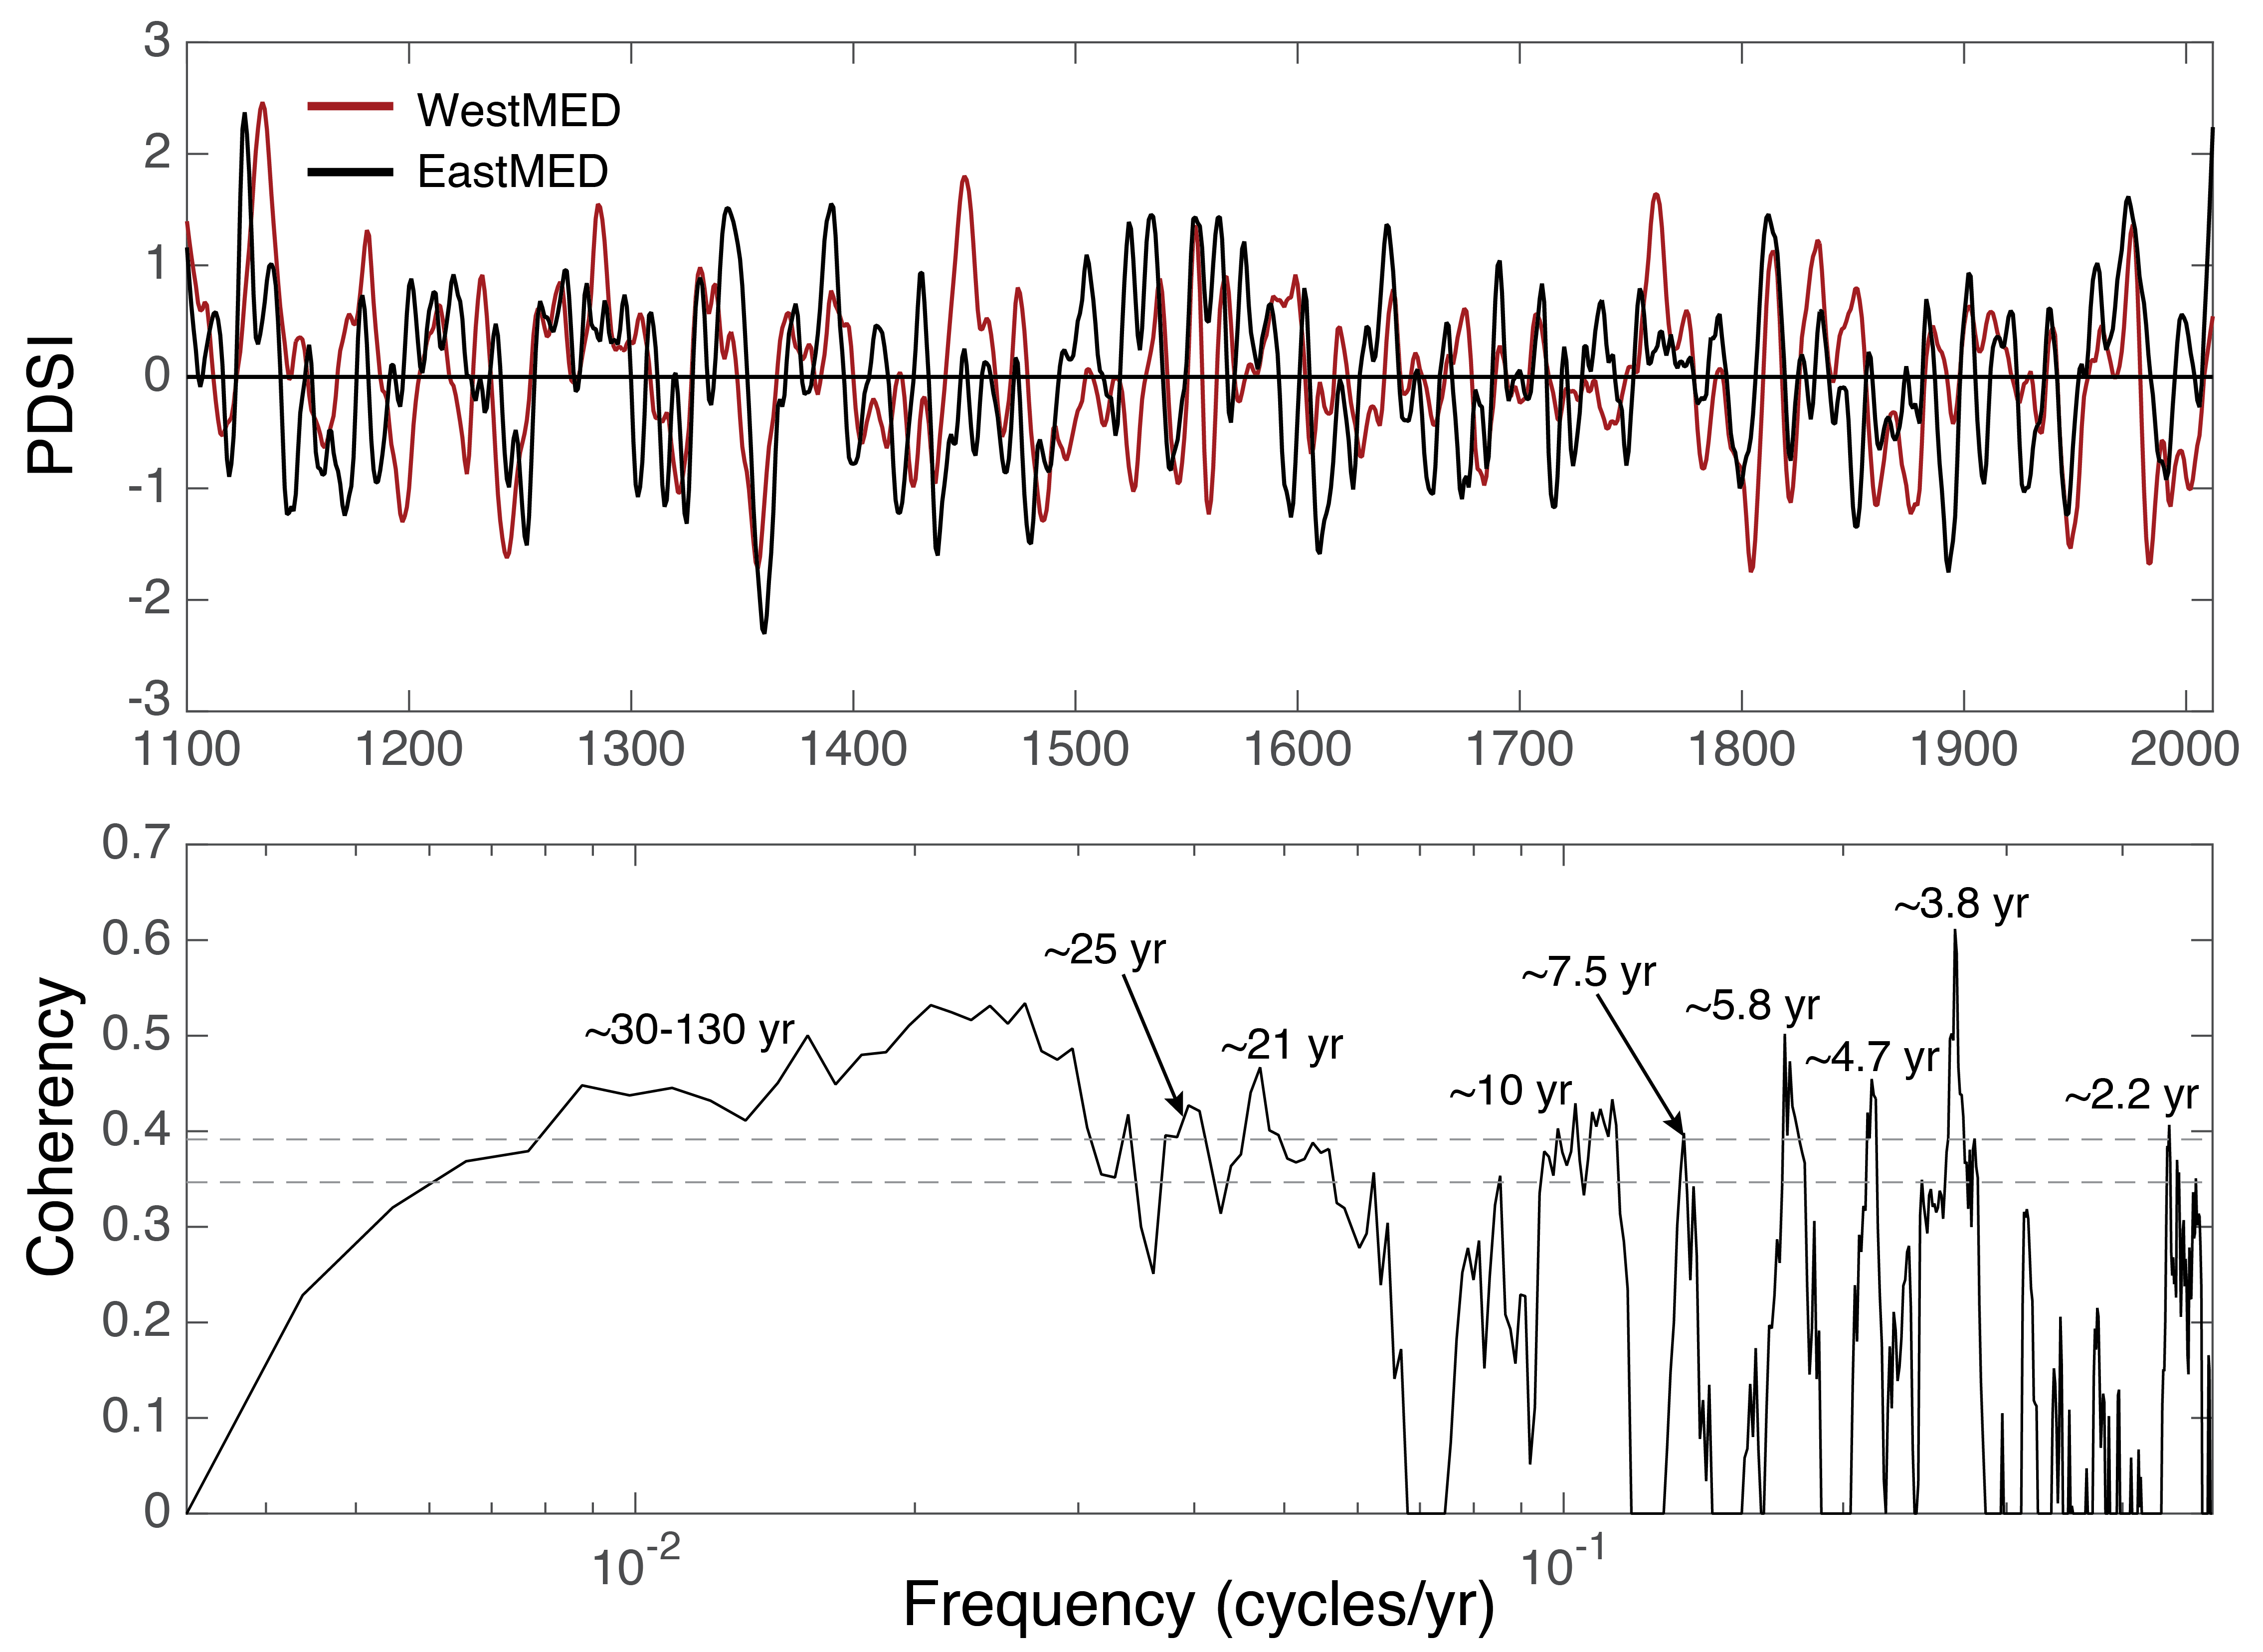
\includegraphics[width=0.9\columnwidth]{fig_09_eastwest_cohere.png}
\caption{Smoothed versions (10-year loess smooth) of the WestMED and EastMED time series (top) and the coherency spectra between the two unsmoothed series (bottom).}\label{placeholder}
\end{figure}

\begin{figure}
\center
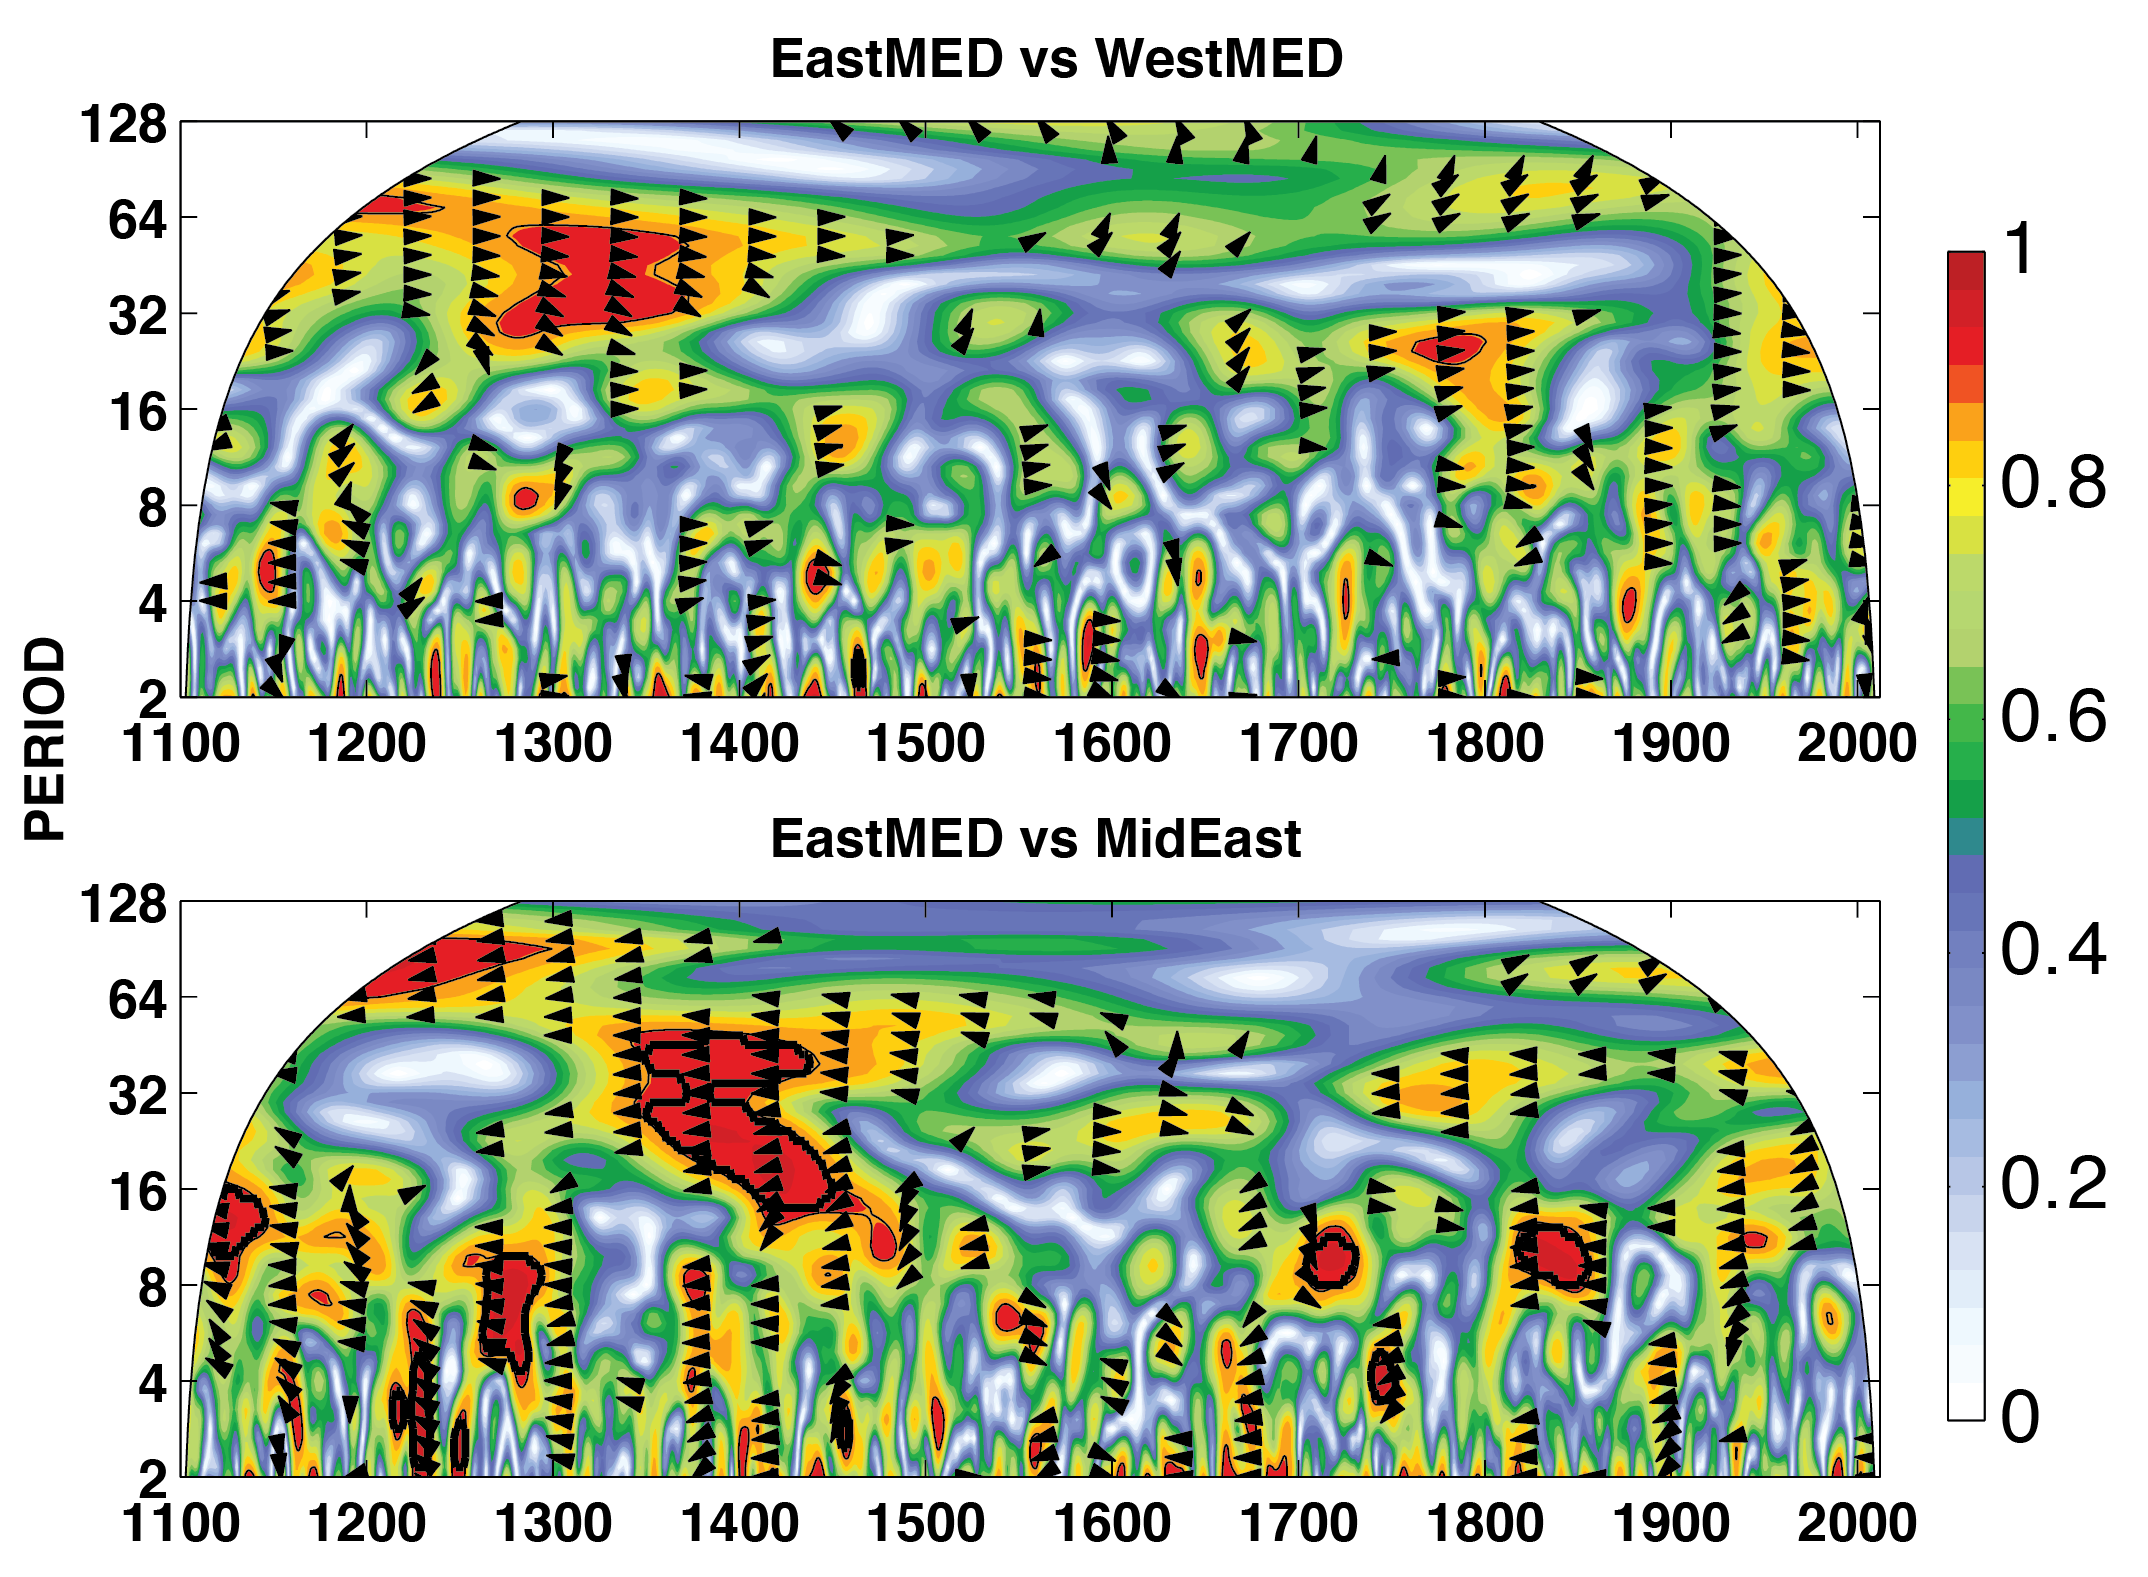
\includegraphics[width=1.0\columnwidth]{fig_10_wavelet_coh.png}
\caption{Squared wavelet coherence for EastMED versus WestMED (top) and EastMED versus MidEast (bottom). Black arrows pointing directly right indicate where the two time series have significant ($p\le0.05$) shared variance and are in phase; black arrows pointed left indicate where the two series are 180 degrees out of phase.}\label{placeholder}
\end{figure}

\begin{figure}
\center
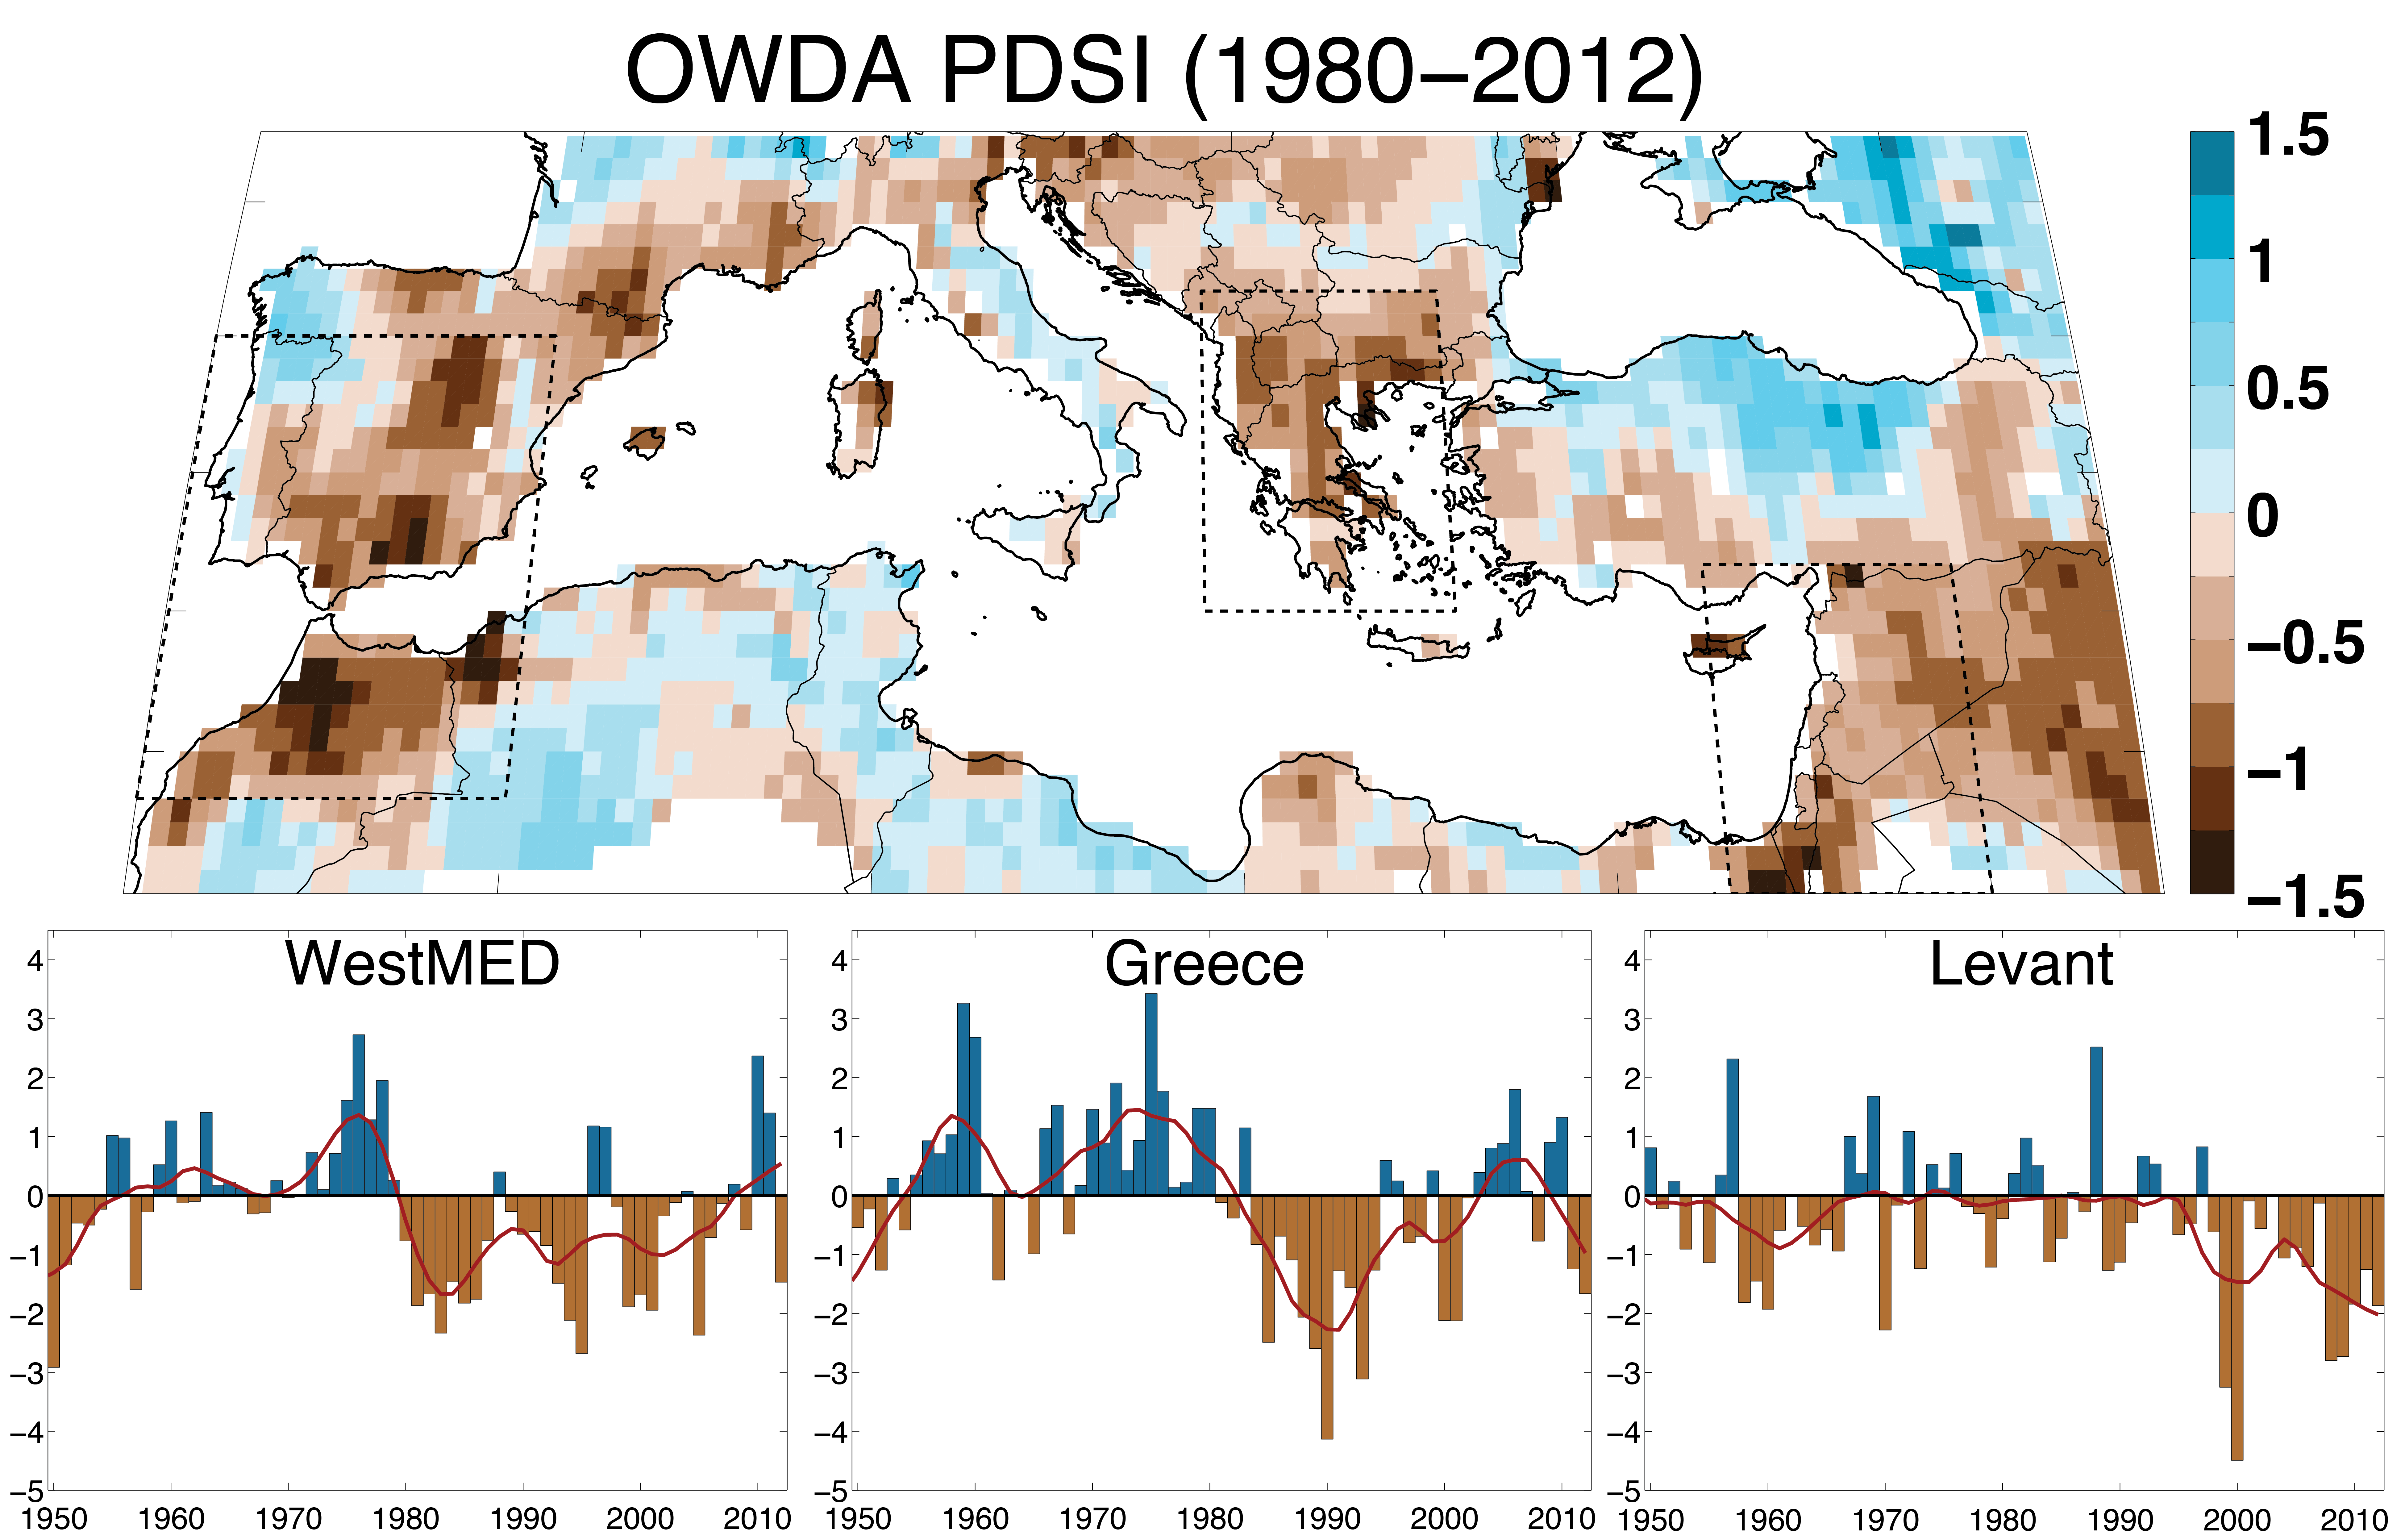
\includegraphics[width=1.0\columnwidth]{fig_11_map_bar_pdsi.png}
\caption{Multi-year average scPDSI for 1980--2012 (top) with regions of recent and persistent drought outlined in dashed black lines: WestMED (32\textsuperscript{o}N--42\textsuperscript{o}N, 10\textsuperscript{o}W--0\textsuperscript{o}), Greece (36\textsuperscript{o}N--43\textsuperscript{o}N, 19\textsuperscript{o}E--26\textsuperscript{o}), and the Levant (30\textsuperscript{o}N--37\textsuperscript{o}N, 33\textsuperscript{o}E--40\textsuperscript{o}E). Also shown (bottom) are the regional average scPDSI time series from these regions for 1950--2012 (red line is a 10-year loess smoother).}\label{placeholder}
\end{figure}

\begin{figure}
\center
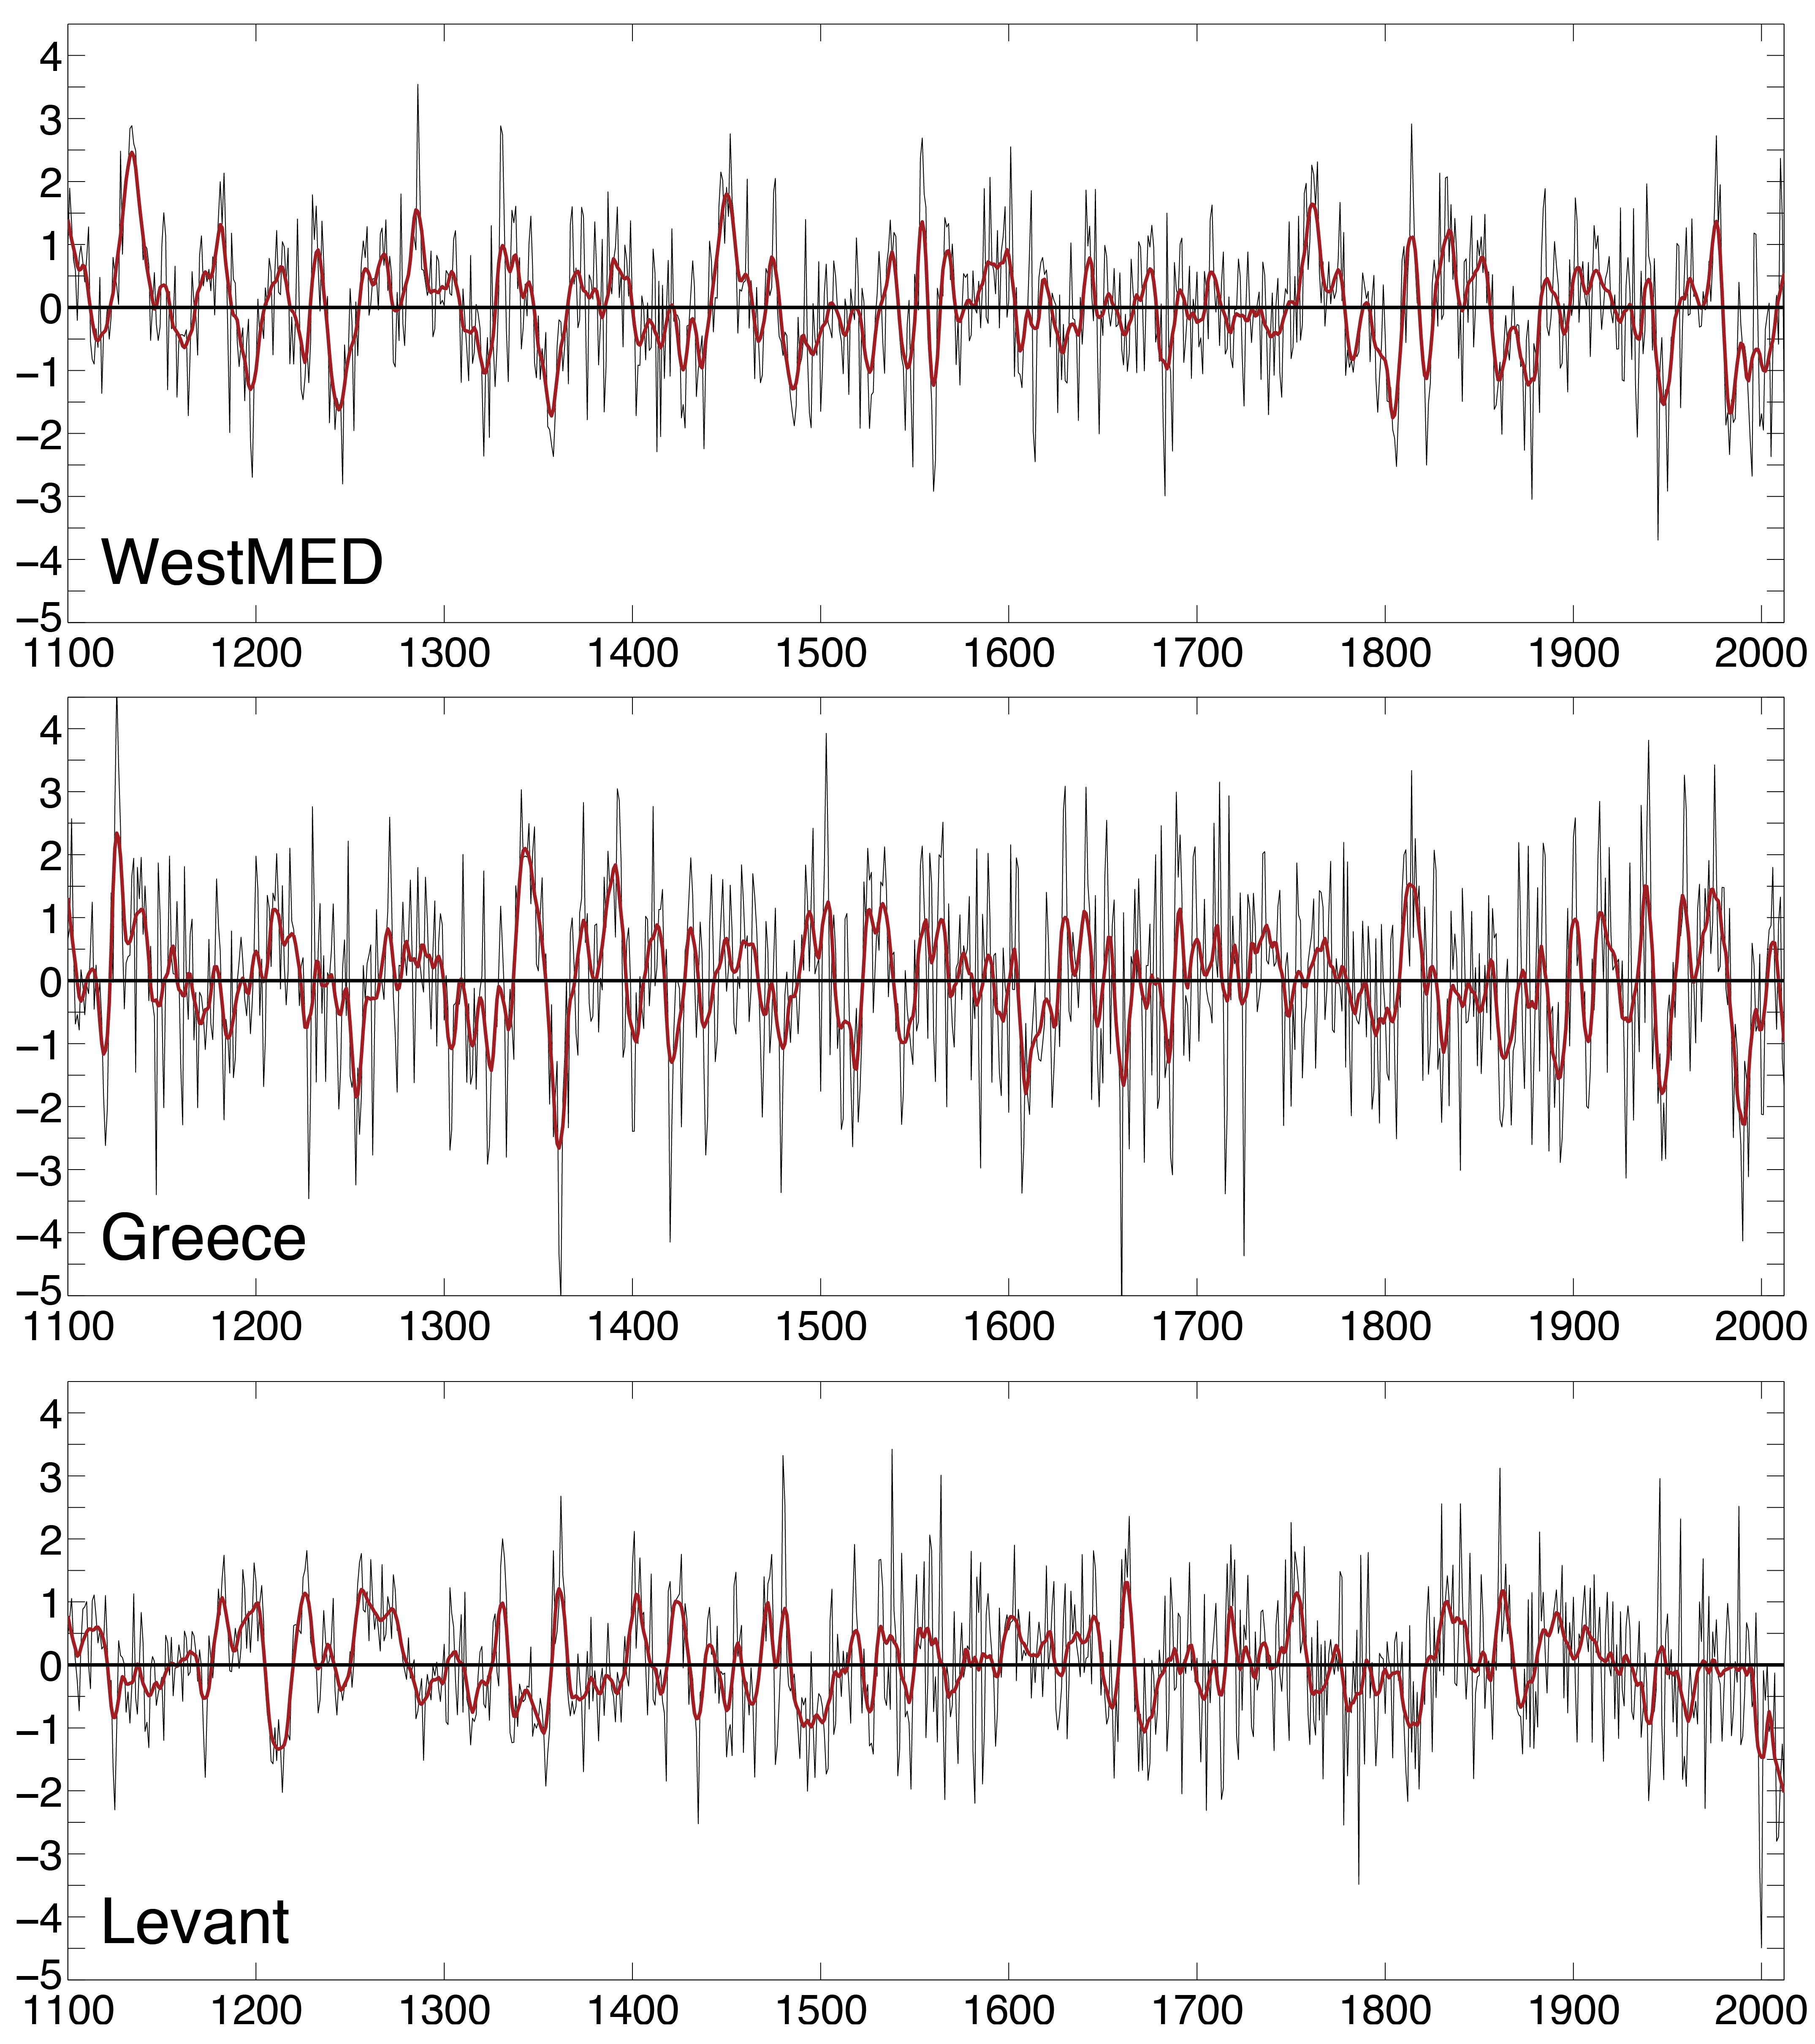
\includegraphics[width=0.9\columnwidth]{fig_12_regional_series_MED1.png}
\caption{Re-centered (zero mean from 1100--2012 CE) time series for WestMED, Greece, and the Levant region. Red lines represent smoothed versions using a 10-year loess smoother.}\label{placeholder}
\end{figure}

\begin{figure}
\center
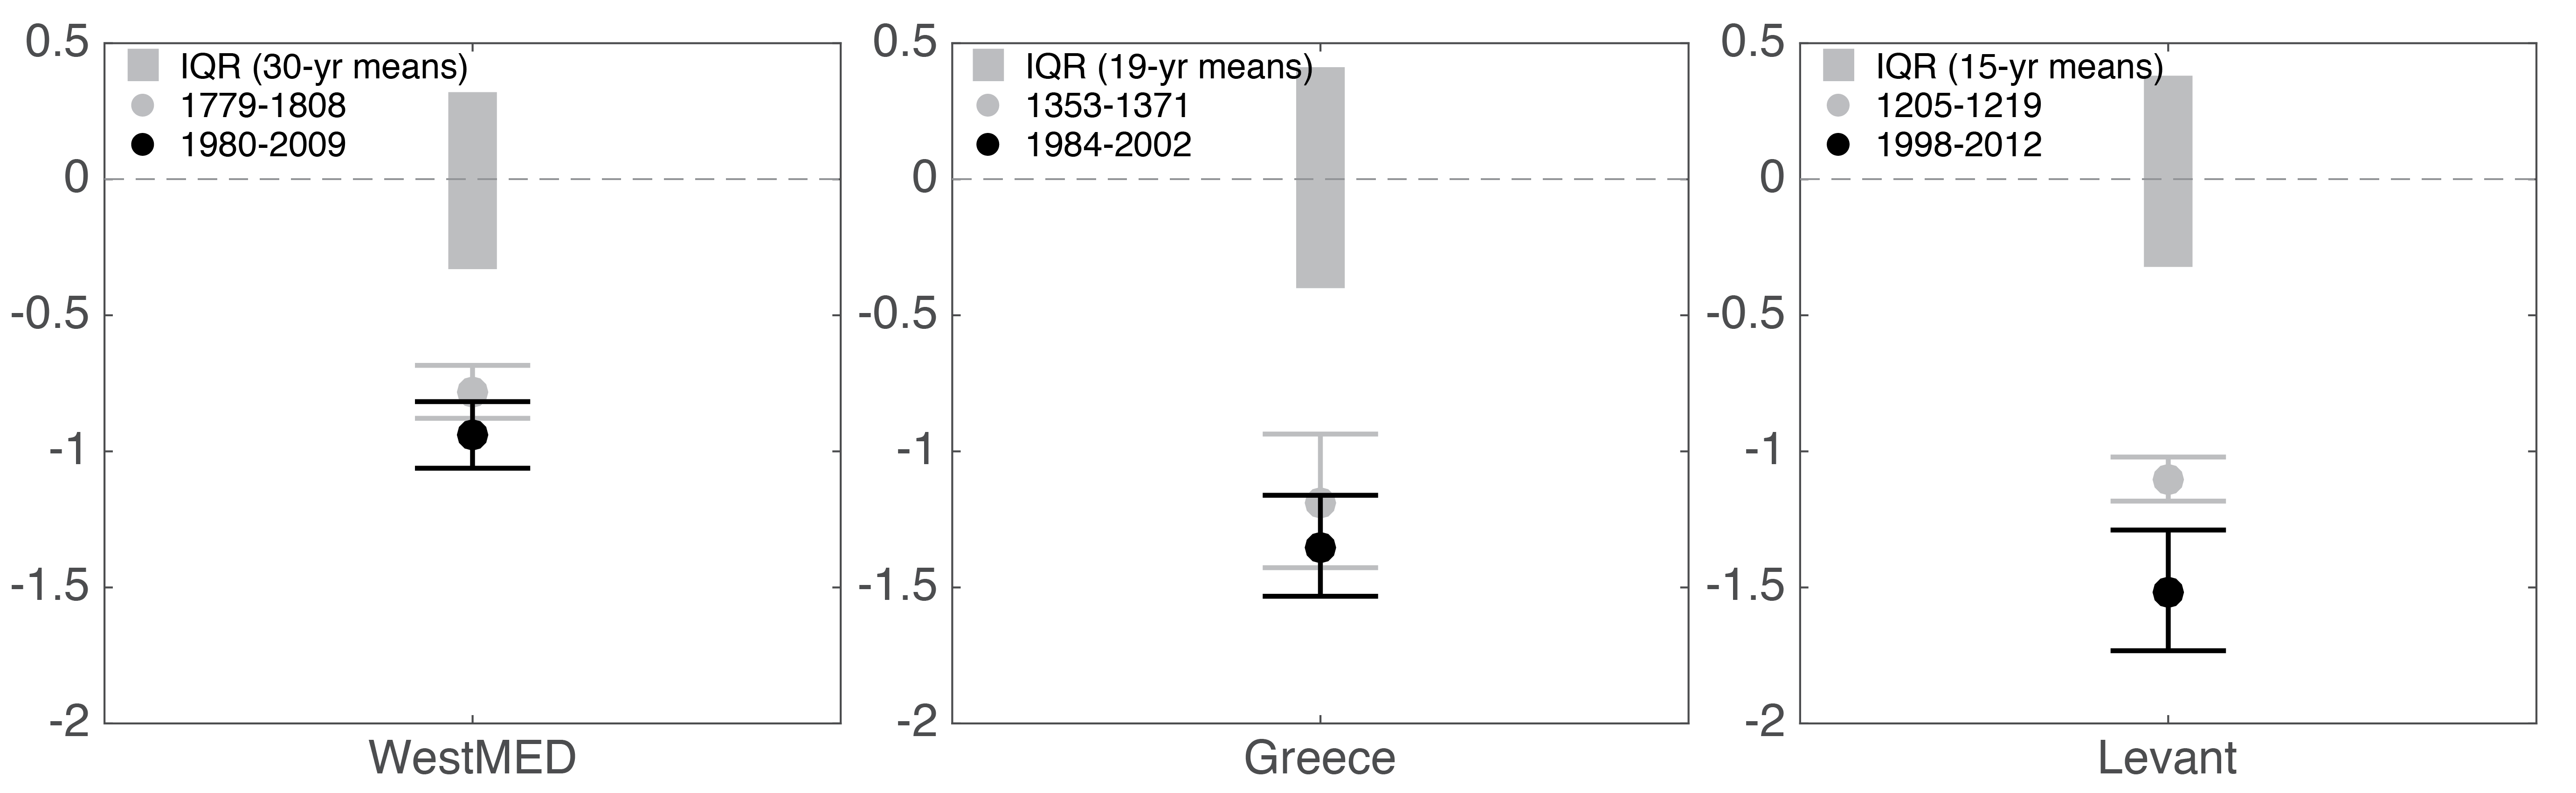
\includegraphics[width=1.0\columnwidth]{fig_13_pdsi_boxplot.png}
\caption{Comparisons between multi-year average re-centered scPDSI during recent decades (black dots) and driest previous periods of the same length in the OWDA from 1100--2012 CE. Grey bars are the interquartile range of mean PDSI for all such periods, grey dots represent the driest period prior to the recent decades, and black dots are the mean PDSI for the most recent drought. Whiskers are the 25\textsuperscript{th} and 75\textsuperscript{th} confidence limits for the dry events, estimated from 10,000 resamplings with replacement from scPDSI values during these intervals.}\label{placeholder}
\end{figure}

%\begin{table}
%\caption{Table caption}\label{sampletable}
%\begin{tabular}{l l l}
%\hline
%\textbf{Treatments} & \textbf{Response 1} & \textbf{Response 2}\\
%\hline
%Treatment 1 & 0.0003262 & 0.562 \\
%Treatment 2 & 0.0015681 & 0.910 \\
%Treatment 3 & 0.0009271 & 0.296 \\
%\hline
%\end{tabular}
%\end{table}

\end{document}

%%%%%%%%%%%%%%%%%%%%%%%%%%%%%%%%%%%%%%%%%%%%%%%%%%%%%%%%%%%%%%%


%% ------------------------------------------------------------------------ %%
%
%  SECTION HEADS
%
%% ------------------------------------------------------------------------ %%

% Capitalize the first letter of each word (except for
% prepositions, conjunctions, and articles that are
% three or fewer letters).

% AGU follows standard outline style; therefore, there cannot be a section 1 without
% a section 2, or a section 2.3.1 without a section 2.3.2.
% Please make sure your section numbers are balanced.
% ---------------
% Level 1 head
%
% Use the \section{} command to identify level 1 heads;
% type the appropriate head wording between the curly
% brackets, as shown below.
%
%An example:
%\section{Level 1 Head: Introduction}
%
% ---------------
% Level 2 head
%
% Use the \subsection{} command to identify level 2 heads.
%An example:
%\subsection{Level 2 Head}
%
% ---------------
% Level 3 head
%
% Use the \subsubsection{} command to identify level 3 heads
%An example:
%\subsubsection{Level 3 Head}
%
%---------------
% Level 4 head
%
% Use the \subsubsubsection{} command to identify level 3 heads
% An example:
%\subsubsubsection{Level 4 Head} An example.
%
%% ------------------------------------------------------------------------ %%
%
%  IN-TEXT LISTS
%
%% ------------------------------------------------------------------------ %%
%
% Do not use bulleted lists; enumerated lists are okay.
% \begin{enumerate}
% \item
% \item
% \item
% \end{enumerate}
%
%% ------------------------------------------------------------------------ %%
%
%  EQUATIONS
%
%% ------------------------------------------------------------------------ %%

% Single-line equations are centered.
% Equation arrays will appear left-aligned.

Math coded inside display math mode \[ ...\]
 will not be numbered, e.g.,:
 \[ x^2=y^2 + z^2\]

 Math coded inside \begin{equation} and \end{equation} will
 be automatically numbered, e.g.,:
 \begin{equation}
 x^2=y^2 + z^2
 \end{equation}

% IF YOU HAVE MULTI-LINE EQUATIONS, PLEASE
% BREAK THE EQUATIONS INTO TWO OR MORE LINES
% OF SINGLE COLUMN WIDTH (20 pc, 8.3 cm)
% using double backslashes (\\).

% To create multiline equations, use the
% \begin{eqnarray} and \end{eqnarray} environment
% as demonstrated below.
\begin{eqnarray}
  x_{1} & = & (x - x_{0}) \cos \Theta \nonumber \\
        && + (y - y_{0}) \sin \Theta  \nonumber \\
  y_{1} & = & -(x - x_{0}) \sin \Theta \nonumber \\
        && + (y - y_{0}) \cos \Theta.
\end{eqnarray}

%If you don't want an equation number, use the star form:
%\begin{eqnarray*}...\end{eqnarray*}

% Break each line at a sign of operation
% (+, -, etc.) if possible, with the sign of operation
% on the new line.

% Indent second and subsequent lines to align with the first character following the equal sign on the first line.

% Use an \hspace{} command to insert horizontal space into your equation if necessary. Place an appropriate unit of measure between the curly braces, e.g. \hspace{1in}; you may have to experiment to achieve the correct amount of space.


%% ------------------------------------------------------------------------ %%
%
%  EQUATION NUMBERING: COUNTER
%
%% ------------------------------------------------------------------------ %%

% You may change equation numbering by resetting
% the equation counter or by explicitly numbering
% an equation.

% To explicitly number an equation, type \eqnum{}
% (with the desired number between the brackets)
% after the \begin{equation} or \begin{eqnarray}
% command.  The \eqnum{} command will affect only
% the equation it appears with; LaTeX will number
% any equations appearing later in the manuscript
% according to the equation counter.
%

% If you have a multiline equation that needs only
% one equation number, use a \nonumber command in
% front of the double backslashes (\\) as shown in
% the multiline equation above.

%% ------------------------------------------------------------------------ %%
%
%  SIDEWAYS FIGURE AND TABLE EXAMPLES
%
%% ------------------------------------------------------------------------ %%
%
% For tables and figures, add \usepackage{rotating} to the paper and add the rotating.sty file to the folder.
% AGU prefers the use of {sidewaystable} over {landscapetable} as it causes fewer problems.
%
% \begin{sidewaysfigure}
% \includegraphics[width=20pc]{samplefigure.eps}
% \caption{caption here}
% \label{label_here}
% \end{sidewaysfigure}
%
% \begin{sidewaystable}
% \caption{}
% \begin{tabular}
% Table layout here.
% \end{tabular}
% \end{sidewaystable}